\documentclass[twoside]{book}

% Packages required by doxygen
\usepackage{fixltx2e}
\usepackage{calc}
\usepackage{doxygen}
\usepackage[export]{adjustbox} % also loads graphicx
\usepackage{graphicx}
\usepackage[utf8]{inputenc}
\usepackage{makeidx}
\usepackage{multicol}
\usepackage{multirow}
\PassOptionsToPackage{warn}{textcomp}
\usepackage{textcomp}
\usepackage[nointegrals]{wasysym}
\usepackage[table]{xcolor}

% Font selection
\usepackage[T1]{fontenc}
\usepackage[scaled=.90]{helvet}
\usepackage{courier}
\usepackage{amssymb}
\usepackage{sectsty}
\renewcommand{\familydefault}{\sfdefault}
\allsectionsfont{%
  \fontseries{bc}\selectfont%
  \color{darkgray}%
}
\renewcommand{\DoxyLabelFont}{%
  \fontseries{bc}\selectfont%
  \color{darkgray}%
}
\newcommand{\+}{\discretionary{\mbox{\scriptsize$\hookleftarrow$}}{}{}}

% Page & text layout
\usepackage{geometry}
\geometry{%
  a4paper,%
  top=2.5cm,%
  bottom=2.5cm,%
  left=2.5cm,%
  right=2.5cm%
}
\tolerance=750
\hfuzz=15pt
\hbadness=750
\setlength{\emergencystretch}{15pt}
\setlength{\parindent}{0cm}
\setlength{\parskip}{3ex plus 2ex minus 2ex}
\makeatletter
\renewcommand{\paragraph}{%
  \@startsection{paragraph}{4}{0ex}{-1.0ex}{1.0ex}{%
    \normalfont\normalsize\bfseries\SS@parafont%
  }%
}
\renewcommand{\subparagraph}{%
  \@startsection{subparagraph}{5}{0ex}{-1.0ex}{1.0ex}{%
    \normalfont\normalsize\bfseries\SS@subparafont%
  }%
}
\makeatother

% Headers & footers
\usepackage{fancyhdr}
\pagestyle{fancyplain}
\fancyhead[LE]{\fancyplain{}{\bfseries\thepage}}
\fancyhead[CE]{\fancyplain{}{}}
\fancyhead[RE]{\fancyplain{}{\bfseries\leftmark}}
\fancyhead[LO]{\fancyplain{}{\bfseries\rightmark}}
\fancyhead[CO]{\fancyplain{}{}}
\fancyhead[RO]{\fancyplain{}{\bfseries\thepage}}
\fancyfoot[LE]{\fancyplain{}{}}
\fancyfoot[CE]{\fancyplain{}{}}
\fancyfoot[RE]{\fancyplain{}{\bfseries\scriptsize Generated by Doxygen }}
\fancyfoot[LO]{\fancyplain{}{\bfseries\scriptsize Generated by Doxygen }}
\fancyfoot[CO]{\fancyplain{}{}}
\fancyfoot[RO]{\fancyplain{}{}}
\renewcommand{\footrulewidth}{0.4pt}
\renewcommand{\chaptermark}[1]{%
  \markboth{#1}{}%
}
\renewcommand{\sectionmark}[1]{%
  \markright{\thesection\ #1}%
}

% Indices & bibliography
\usepackage{natbib}
\usepackage[titles]{tocloft}
\setcounter{tocdepth}{3}
\setcounter{secnumdepth}{5}
\makeindex

% Hyperlinks (required, but should be loaded last)
\usepackage{ifpdf}
\ifpdf
  \usepackage[pdftex,pagebackref=true]{hyperref}
\else
  \usepackage[ps2pdf,pagebackref=true]{hyperref}
\fi
\hypersetup{%
  colorlinks=true,%
  linkcolor=blue,%
  citecolor=blue,%
  unicode%
}

% Custom commands
\newcommand{\clearemptydoublepage}{%
  \newpage{\pagestyle{empty}\cleardoublepage}%
}

\usepackage{caption}
\captionsetup{labelsep=space,justification=centering,font={bf},singlelinecheck=off,skip=4pt,position=top}

%===== C O N T E N T S =====

\begin{document}

% Titlepage & ToC
\hypersetup{pageanchor=false,
             bookmarksnumbered=true,
             pdfencoding=unicode
            }
\pagenumbering{alph}
\begin{titlepage}
\vspace*{7cm}
\begin{center}%
{\Large My Project }\\
\vspace*{1cm}
{\large Generated by Doxygen 1.8.13}\\
\end{center}
\end{titlepage}
\clearemptydoublepage
\pagenumbering{roman}
\tableofcontents
\clearemptydoublepage
\pagenumbering{arabic}
\hypersetup{pageanchor=true}

%--- Begin generated contents ---
\chapter{Namespace Index}
\section{Namespace List}
Here is a list of all documented namespaces with brief descriptions\+:\begin{DoxyCompactList}
\item\contentsline{section}{\mbox{\hyperlink{namespace_pz_g}{PzG}} \\*Moduł narzędzi umożliwiających połącznie z G\+N\+U\+Plotem }{\pageref{namespace_pz_g}}{}
\end{DoxyCompactList}

\chapter{Class Index}
\section{Class List}
Here are the classes, structs, unions and interfaces with brief descriptions\+:\begin{DoxyCompactList}
\item\contentsline{section}{\hyperlink{structelement__sekwencji}{element\+\_\+sekwencji} }{\pageref{structelement__sekwencji}}{}
\item\contentsline{section}{\hyperlink{classPzG_1_1InfoPlikuDoRysowania}{Pz\+G\+::\+Info\+Pliku\+Do\+Rysowania} \\*Zestaw informacji dotyczący pliku i sposobu rysowania }{\pageref{classPzG_1_1InfoPlikuDoRysowania}}{}
\item\contentsline{section}{\hyperlink{classPzG_1_1LaczeDoGNUPlota}{Pz\+G\+::\+Lacze\+Do\+G\+N\+U\+Plota} \\*Klasa realizuje interfejs do programu G\+N\+U\+Plot }{\pageref{classPzG_1_1LaczeDoGNUPlota}}{}
\item\contentsline{section}{\hyperlink{classMacierz}{Macierz$<$ Wymiar $>$} \\*Szablon klasy macierz Szablon klasy macierz jest reprezentacja macierzy w przestrzeni n-\/ wymiarowej gdzie n jest reprezenowana przez argument szablonu wymiar }{\pageref{classMacierz}}{}
\item\contentsline{section}{\hyperlink{classProstopadloscian}{Prostopadloscian} \\*Klasa prostopadloscian Klasa prostopadloscian jest reprezentacja prostopadloscianu w przestrzeni 3D }{\pageref{classProstopadloscian}}{}
\item\contentsline{section}{\hyperlink{classWektor}{Wektor$<$ Wymiar $>$} \\*Szablon klasy wektor Szablon klasy wektor jest reprezentacja wektoru w przestrzeni n-\/ wymiarowej gdzie n jest reprezenowana przez argument szablonu wymiar }{\pageref{classWektor}}{}
\end{DoxyCompactList}

\chapter{File Index}
\section{File List}
Here is a list of all documented files with brief descriptions\+:\begin{DoxyCompactList}
\item\contentsline{section}{inc/\mbox{\hyperlink{_dron_8hh}{Dron.\+hh}} }{\pageref{_dron_8hh}}{}
\item\contentsline{section}{inc/\mbox{\hyperlink{_fabryka__obiektow_8hh}{Fabryka\+\_\+obiektow.\+hh}} }{\pageref{_fabryka__obiektow_8hh}}{}
\item\contentsline{section}{inc/\mbox{\hyperlink{_graniastoslup_8hh}{Graniastoslup.\+hh}} }{\pageref{_graniastoslup_8hh}}{}
\item\contentsline{section}{inc/\mbox{\hyperlink{_korpus_8hh}{Korpus.\+hh}} }{\pageref{_korpus_8hh}}{}
\item\contentsline{section}{inc/\mbox{\hyperlink{lacze__do__gnuplota_8hh}{lacze\+\_\+do\+\_\+gnuplota.\+hh}} }{\pageref{lacze__do__gnuplota_8hh}}{}
\item\contentsline{section}{inc/\mbox{\hyperlink{_macierz_8hh}{Macierz.\+hh}} }{\pageref{_macierz_8hh}}{}
\item\contentsline{section}{inc/{\bfseries Macierz3x3.\+hh} }{\pageref{_macierz3x3_8hh}}{}
\item\contentsline{section}{inc/\mbox{\hyperlink{_obiektsceny_8hh}{Obiektsceny.\+hh}} }{\pageref{_obiektsceny_8hh}}{}
\item\contentsline{section}{inc/\mbox{\hyperlink{_prostopadloscian_8hh}{Prostopadloscian.\+hh}} }{\pageref{_prostopadloscian_8hh}}{}
\item\contentsline{section}{inc/{\bfseries Przeszkoda.\+hh} }{\pageref{_przeszkoda_8hh}}{}
\item\contentsline{section}{inc/\mbox{\hyperlink{_scena_8hh}{Scena.\+hh}} }{\pageref{_scena_8hh}}{}
\item\contentsline{section}{inc/\mbox{\hyperlink{_wektor_8hh}{Wektor.\+hh}} }{\pageref{_wektor_8hh}}{}
\item\contentsline{section}{inc/{\bfseries Wektor3\+D.\+hh} }{\pageref{_wektor3_d_8hh}}{}
\item\contentsline{section}{inc/\mbox{\hyperlink{_wirnik_8hh}{Wirnik.\+hh}} }{\pageref{_wirnik_8hh}}{}
\end{DoxyCompactList}

\chapter{Namespace Documentation}
\hypertarget{namespacePzG}{}\section{PzG Namespace Reference}
\label{namespacePzG}\index{PzG@{PzG}}


Moduł narzędzi umożliwiających połącznie z G\+N\+U\+Plotem.  


\subsection*{Classes}
\begin{DoxyCompactItemize}
\item 
class \hyperlink{classPzG_1_1InfoPlikuDoRysowania}{Info\+Pliku\+Do\+Rysowania}
\begin{DoxyCompactList}\small\item\em Zestaw informacji dotyczący pliku i sposobu rysowania. \end{DoxyCompactList}\item 
class \hyperlink{classPzG_1_1LaczeDoGNUPlota}{Lacze\+Do\+G\+N\+U\+Plota}
\begin{DoxyCompactList}\small\item\em Klasa realizuje interfejs do programu G\+N\+U\+Plot. \end{DoxyCompactList}\end{DoxyCompactItemize}
\subsection*{Enumerations}
\begin{DoxyCompactItemize}
\item 
enum \hyperlink{namespacePzG_aeedae1ef10c66d720f9e89de408ca4ca}{Tryb\+Rysowania} \{ {\bfseries T\+R\+\_\+2D}, 
{\bfseries T\+R\+\_\+3D}
 \}\begin{DoxyCompactList}\small\item\em Określa tryb rysowania realizowanego przez program {\ttfamily gnuplot}. \end{DoxyCompactList}
\item 
enum \hyperlink{namespacePzG_a705c92106f39b7d0c34a6739d10ff0b6}{Rodzaj\+Rysowania} \{ {\bfseries R\+R\+\_\+\+Ciagly}, 
{\bfseries R\+R\+\_\+\+Punktowy}
 \}\begin{DoxyCompactList}\small\item\em Sposób rysowania linii. \end{DoxyCompactList}
\end{DoxyCompactItemize}
\subsection*{Functions}
\begin{DoxyCompactItemize}
\item 
\mbox{\Hypertarget{namespacePzG_ae1ae4d36f66c77879380ba73da8e20e3}\label{namespacePzG_ae1ae4d36f66c77879380ba73da8e20e3}} 
bool {\bfseries Czy\+Jest\+Plik} (char const $\ast$Nazwa\+Pliku)
\end{DoxyCompactItemize}


\subsection{Detailed Description}
Moduł narzędzi umożliwiających połącznie z G\+N\+U\+Plotem. 

Niniejsza przestrzeń nazw stanowi moduł logiczny zawierający narzędzia umożliwiające realizację połączenia z programem {\ttfamily gnuplot}. 

\subsection{Enumeration Type Documentation}
\mbox{\Hypertarget{namespacePzG_a705c92106f39b7d0c34a6739d10ff0b6}\label{namespacePzG_a705c92106f39b7d0c34a6739d10ff0b6}} 
\index{PzG@{PzG}!Rodzaj\+Rysowania@{Rodzaj\+Rysowania}}
\index{Rodzaj\+Rysowania@{Rodzaj\+Rysowania}!PzG@{PzG}}
\subsubsection{\texorpdfstring{Rodzaj\+Rysowania}{RodzajRysowania}}
{\footnotesize\ttfamily enum \hyperlink{namespacePzG_a705c92106f39b7d0c34a6739d10ff0b6}{Pz\+G\+::\+Rodzaj\+Rysowania}}



Sposób rysowania linii. 

Określa sposób rysowania linii. \mbox{\Hypertarget{namespacePzG_aeedae1ef10c66d720f9e89de408ca4ca}\label{namespacePzG_aeedae1ef10c66d720f9e89de408ca4ca}} 
\index{PzG@{PzG}!Tryb\+Rysowania@{Tryb\+Rysowania}}
\index{Tryb\+Rysowania@{Tryb\+Rysowania}!PzG@{PzG}}
\subsubsection{\texorpdfstring{Tryb\+Rysowania}{TrybRysowania}}
{\footnotesize\ttfamily enum \hyperlink{namespacePzG_aeedae1ef10c66d720f9e89de408ca4ca}{Pz\+G\+::\+Tryb\+Rysowania}}



Określa tryb rysowania realizowanego przez program {\ttfamily gnuplot}. 

Typ wyliczeniowy określające dopuszczalne tryby rysowania realizowanego przez program {\ttfamily gnuplot}. Wybór trybu wiąże się ze zmianą sposobu interpretacji danych zawartych pliku. Jeśli np. wybrany zostanie tryb 2D, to zakłada się, że w każdej linii pliku z danymi znajdują się wartości współrzędnych {\itshape x}, {\itshape y}. Wartości typu\+: \begin{DoxyItemize}
\item {\ttfamily T\+R\+\_\+2D} -\/ rysowanie w trybie 2D, co sprowadza się do rysowania wykresów funkcji jednej zmiennej. \item {\ttfamily T\+R\+\_\+3D} -\/ rysowanie w trybie 3D. Oznacza to możliwość rysowania wykresów funkcji dwóch zmiennych. \end{DoxyItemize}

\chapter{Class Documentation}
\hypertarget{structelement__sekwencji}{}\section{element\+\_\+sekwencji Struct Reference}
\label{structelement__sekwencji}\index{element\+\_\+sekwencji@{element\+\_\+sekwencji}}
\subsection*{Public Attributes}
\begin{DoxyCompactItemize}
\item 
\mbox{\Hypertarget{structelement__sekwencji_a3e4e0297377fc8fc44142ba73a8a0165}\label{structelement__sekwencji_a3e4e0297377fc8fc44142ba73a8a0165}} 
char {\bfseries os}
\item 
\mbox{\Hypertarget{structelement__sekwencji_a22bf3d71d66f3a92bfab955d453cbe7c}\label{structelement__sekwencji_a22bf3d71d66f3a92bfab955d453cbe7c}} 
int {\bfseries kat}
\end{DoxyCompactItemize}


The documentation for this struct was generated from the following file\+:\begin{DoxyCompactItemize}
\item 
src/\hyperlink{main_8cpp}{main.\+cpp}\end{DoxyCompactItemize}

\hypertarget{classPzG_1_1InfoPlikuDoRysowania}{}\section{PzG\+:\+:Info\+Pliku\+Do\+Rysowania Class Reference}
\label{classPzG_1_1InfoPlikuDoRysowania}\index{Pz\+G\+::\+Info\+Pliku\+Do\+Rysowania@{Pz\+G\+::\+Info\+Pliku\+Do\+Rysowania}}


Zestaw informacji dotyczący pliku i sposobu rysowania.  




{\ttfamily \#include $<$lacze\+\_\+do\+\_\+gnuplota.\+hh$>$}

\subsection*{Public Member Functions}
\begin{DoxyCompactItemize}
\item 
\hyperlink{classPzG_1_1InfoPlikuDoRysowania_a48bc8ad94ef5fd5120b668a566c9172e}{Info\+Pliku\+Do\+Rysowania} (const char $\ast$Nazwa\+Pliku, \hyperlink{namespacePzG_a705c92106f39b7d0c34a6739d10ff0b6}{Rodzaj\+Rysowania} Rodz\+Rys, int Szerokosc)
\item 
const std\+::string \hyperlink{classPzG_1_1InfoPlikuDoRysowania_ac92a5dc258f9b6164631e2ea5247a7a7}{Wez\+Nazwe\+Pliku} () const
\begin{DoxyCompactList}\small\item\em Udostępia nazwę pliku do rysowania. \end{DoxyCompactList}\item 
void \hyperlink{classPzG_1_1InfoPlikuDoRysowania_ae734c69f5cecf9c0584e3a7f433340ea}{Zmien\+Nazwe\+Pliku} (const std\+::string \&Nazwa\+Pliku)
\begin{DoxyCompactList}\small\item\em Zmienia nazwę pliku do rysowania. \end{DoxyCompactList}\item 
\hyperlink{namespacePzG_a705c92106f39b7d0c34a6739d10ff0b6}{Rodzaj\+Rysowania} \hyperlink{classPzG_1_1InfoPlikuDoRysowania_a6a46f3c7b7a08dfa9d694f387f873234}{Wez\+Rodz\+Rys} () const
\begin{DoxyCompactList}\small\item\em Udostępnia sposób rysowanej linii. \end{DoxyCompactList}\item 
int \hyperlink{classPzG_1_1InfoPlikuDoRysowania_a627bb615c50f3b03374774e6b974488b}{Wez\+Szerokosc} () const
\begin{DoxyCompactList}\small\item\em Udostępnia informację o szerokości linii. \end{DoxyCompactList}\end{DoxyCompactItemize}


\subsection{Detailed Description}
Zestaw informacji dotyczący pliku i sposobu rysowania. 

Klasa modeluje zestaw informacji dotyczący pliku i sposobu w jaki mają być wizualizowane zawarte w nim dane. 

\subsection{Constructor \& Destructor Documentation}
\mbox{\Hypertarget{classPzG_1_1InfoPlikuDoRysowania_a48bc8ad94ef5fd5120b668a566c9172e}\label{classPzG_1_1InfoPlikuDoRysowania_a48bc8ad94ef5fd5120b668a566c9172e}} 
\index{Pz\+G\+::\+Info\+Pliku\+Do\+Rysowania@{Pz\+G\+::\+Info\+Pliku\+Do\+Rysowania}!Info\+Pliku\+Do\+Rysowania@{Info\+Pliku\+Do\+Rysowania}}
\index{Info\+Pliku\+Do\+Rysowania@{Info\+Pliku\+Do\+Rysowania}!Pz\+G\+::\+Info\+Pliku\+Do\+Rysowania@{Pz\+G\+::\+Info\+Pliku\+Do\+Rysowania}}
\subsubsection{\texorpdfstring{Info\+Pliku\+Do\+Rysowania()}{InfoPlikuDoRysowania()}}
{\footnotesize\ttfamily Pz\+G\+::\+Info\+Pliku\+Do\+Rysowania\+::\+Info\+Pliku\+Do\+Rysowania (\begin{DoxyParamCaption}\item[{const char $\ast$}]{Nazwa\+Pliku,  }\item[{\hyperlink{namespacePzG_a705c92106f39b7d0c34a6739d10ff0b6}{Rodzaj\+Rysowania}}]{Rodz\+Rys,  }\item[{int}]{Szerokosc }\end{DoxyParamCaption})\hspace{0.3cm}{\ttfamily [inline]}}

Inicjalizuje obiekt. 
\begin{DoxyParams}{Parameters}
{\em Nazwa\+Pliku} & -\/ nazwa pliku, z którego pobierane będą dane, \\
\hline
{\em Rodz\+Rys} & -\/ rodzaj rysowania linii, \\
\hline
{\em Szerokosc} & -\/ szerokosc linii. \\
\hline
\end{DoxyParams}


\subsection{Member Function Documentation}
\mbox{\Hypertarget{classPzG_1_1InfoPlikuDoRysowania_ac92a5dc258f9b6164631e2ea5247a7a7}\label{classPzG_1_1InfoPlikuDoRysowania_ac92a5dc258f9b6164631e2ea5247a7a7}} 
\index{Pz\+G\+::\+Info\+Pliku\+Do\+Rysowania@{Pz\+G\+::\+Info\+Pliku\+Do\+Rysowania}!Wez\+Nazwe\+Pliku@{Wez\+Nazwe\+Pliku}}
\index{Wez\+Nazwe\+Pliku@{Wez\+Nazwe\+Pliku}!Pz\+G\+::\+Info\+Pliku\+Do\+Rysowania@{Pz\+G\+::\+Info\+Pliku\+Do\+Rysowania}}
\subsubsection{\texorpdfstring{Wez\+Nazwe\+Pliku()}{WezNazwePliku()}}
{\footnotesize\ttfamily const std\+::string Pz\+G\+::\+Info\+Pliku\+Do\+Rysowania\+::\+Wez\+Nazwe\+Pliku (\begin{DoxyParamCaption}{ }\end{DoxyParamCaption}) const\hspace{0.3cm}{\ttfamily [inline]}}



Udostępia nazwę pliku do rysowania. 

Udostępnia nazwę pliku z danymi do rysowania. \mbox{\Hypertarget{classPzG_1_1InfoPlikuDoRysowania_a6a46f3c7b7a08dfa9d694f387f873234}\label{classPzG_1_1InfoPlikuDoRysowania_a6a46f3c7b7a08dfa9d694f387f873234}} 
\index{Pz\+G\+::\+Info\+Pliku\+Do\+Rysowania@{Pz\+G\+::\+Info\+Pliku\+Do\+Rysowania}!Wez\+Rodz\+Rys@{Wez\+Rodz\+Rys}}
\index{Wez\+Rodz\+Rys@{Wez\+Rodz\+Rys}!Pz\+G\+::\+Info\+Pliku\+Do\+Rysowania@{Pz\+G\+::\+Info\+Pliku\+Do\+Rysowania}}
\subsubsection{\texorpdfstring{Wez\+Rodz\+Rys()}{WezRodzRys()}}
{\footnotesize\ttfamily \hyperlink{namespacePzG_a705c92106f39b7d0c34a6739d10ff0b6}{Rodzaj\+Rysowania} Pz\+G\+::\+Info\+Pliku\+Do\+Rysowania\+::\+Wez\+Rodz\+Rys (\begin{DoxyParamCaption}{ }\end{DoxyParamCaption}) const\hspace{0.3cm}{\ttfamily [inline]}}



Udostępnia sposób rysowanej linii. 

Udostępnia informację o sposóbie rysowania linii. \mbox{\Hypertarget{classPzG_1_1InfoPlikuDoRysowania_a627bb615c50f3b03374774e6b974488b}\label{classPzG_1_1InfoPlikuDoRysowania_a627bb615c50f3b03374774e6b974488b}} 
\index{Pz\+G\+::\+Info\+Pliku\+Do\+Rysowania@{Pz\+G\+::\+Info\+Pliku\+Do\+Rysowania}!Wez\+Szerokosc@{Wez\+Szerokosc}}
\index{Wez\+Szerokosc@{Wez\+Szerokosc}!Pz\+G\+::\+Info\+Pliku\+Do\+Rysowania@{Pz\+G\+::\+Info\+Pliku\+Do\+Rysowania}}
\subsubsection{\texorpdfstring{Wez\+Szerokosc()}{WezSzerokosc()}}
{\footnotesize\ttfamily int Pz\+G\+::\+Info\+Pliku\+Do\+Rysowania\+::\+Wez\+Szerokosc (\begin{DoxyParamCaption}{ }\end{DoxyParamCaption}) const\hspace{0.3cm}{\ttfamily [inline]}}



Udostępnia informację o szerokości linii. 

Udostępnia informację o szerokości rysowanej linii. \mbox{\Hypertarget{classPzG_1_1InfoPlikuDoRysowania_ae734c69f5cecf9c0584e3a7f433340ea}\label{classPzG_1_1InfoPlikuDoRysowania_ae734c69f5cecf9c0584e3a7f433340ea}} 
\index{Pz\+G\+::\+Info\+Pliku\+Do\+Rysowania@{Pz\+G\+::\+Info\+Pliku\+Do\+Rysowania}!Zmien\+Nazwe\+Pliku@{Zmien\+Nazwe\+Pliku}}
\index{Zmien\+Nazwe\+Pliku@{Zmien\+Nazwe\+Pliku}!Pz\+G\+::\+Info\+Pliku\+Do\+Rysowania@{Pz\+G\+::\+Info\+Pliku\+Do\+Rysowania}}
\subsubsection{\texorpdfstring{Zmien\+Nazwe\+Pliku()}{ZmienNazwePliku()}}
{\footnotesize\ttfamily void Pz\+G\+::\+Info\+Pliku\+Do\+Rysowania\+::\+Zmien\+Nazwe\+Pliku (\begin{DoxyParamCaption}\item[{const std\+::string \&}]{Nazwa\+Pliku }\end{DoxyParamCaption})\hspace{0.3cm}{\ttfamily [inline]}}



Zmienia nazwę pliku do rysowania. 

Zmienia nazwę pliku z danymi do rysowania. 

The documentation for this class was generated from the following file\+:\begin{DoxyCompactItemize}
\item 
inc/\hyperlink{lacze__do__gnuplota_8hh}{lacze\+\_\+do\+\_\+gnuplota.\+hh}\end{DoxyCompactItemize}

\hypertarget{classPzG_1_1LaczeDoGNUPlota}{}\section{PzG\+:\+:Lacze\+Do\+G\+N\+U\+Plota Class Reference}
\label{classPzG_1_1LaczeDoGNUPlota}\index{Pz\+G\+::\+Lacze\+Do\+G\+N\+U\+Plota@{Pz\+G\+::\+Lacze\+Do\+G\+N\+U\+Plota}}


Klasa realizuje interfejs do programu G\+N\+U\+Plot.  




{\ttfamily \#include $<$lacze\+\_\+do\+\_\+gnuplota.\+hh$>$}

\subsection*{Public Member Functions}
\begin{DoxyCompactItemize}
\item 
void \hyperlink{classPzG_1_1LaczeDoGNUPlota_a11421d7c67deab6b7524cc492407e897}{Pokaz\+Os\+\_\+\+OX} (bool Pokaz)
\begin{DoxyCompactList}\small\item\em Umożliwia lub zabrania rysowania osi OX. \end{DoxyCompactList}\item 
bool \hyperlink{classPzG_1_1LaczeDoGNUPlota_ae112972af57167c3b053bf922bce6bbf}{Pokaz\+Os\+\_\+\+OX} () const
\begin{DoxyCompactList}\small\item\em Czy oś OX ma być rysowana. \end{DoxyCompactList}\item 
void \hyperlink{classPzG_1_1LaczeDoGNUPlota_a7c3db909b266fc30808e86406c04b516}{Pokaz\+Os\+\_\+\+OY} (bool Pokaz)
\begin{DoxyCompactList}\small\item\em Umożliwia lub zabrania rysowania osi OY. \end{DoxyCompactList}\item 
bool \hyperlink{classPzG_1_1LaczeDoGNUPlota_a7298f469f6932f5c808dcf620650b4b8}{Pokaz\+Os\+\_\+\+OY} () const
\begin{DoxyCompactList}\small\item\em Czy oś OY ma być rysowana. \end{DoxyCompactList}\item 
void \hyperlink{classPzG_1_1LaczeDoGNUPlota_a9fabfe88cb1801a5de8923f45f514b99}{Pokaz\+Os\+\_\+\+OZ} (bool Pokaz)
\begin{DoxyCompactList}\small\item\em Umożliwia lub zabrania rysowania osi OZ. \end{DoxyCompactList}\item 
bool \hyperlink{classPzG_1_1LaczeDoGNUPlota_a22c708af33c57bf3b5d1b4e82b4017b7}{Pokaz\+Os\+\_\+\+OZ} () const
\begin{DoxyCompactList}\small\item\em Czy oś OZ ma być rysowana. \end{DoxyCompactList}\item 
float \hyperlink{classPzG_1_1LaczeDoGNUPlota_a66836c9749bf179420e4ca3e9447efd7}{Xmin} () const
\item 
float \hyperlink{classPzG_1_1LaczeDoGNUPlota_a8e23479629af3df3d352b7839ae396b8}{Xmax} () const
\item 
float \hyperlink{classPzG_1_1LaczeDoGNUPlota_a9352c0382bfaeaaba9f65399a7383164}{Ymin} () const
\item 
float \hyperlink{classPzG_1_1LaczeDoGNUPlota_ac54e4e7448ce3bd324efdc94a999f535}{Ymax} () const
\item 
float \hyperlink{classPzG_1_1LaczeDoGNUPlota_a9068bd9a9873ba9c6d70016f1ae7cd7f}{Zmin} () const
\item 
float \hyperlink{classPzG_1_1LaczeDoGNUPlota_a20a5d03e1fc19c682032bffc54340f12}{Zmax} () const
\item 
void \hyperlink{classPzG_1_1LaczeDoGNUPlota_a10950349b348fd3a3d4143e95337527c}{Zmien\+Tryb\+Rys} (\hyperlink{namespacePzG_aeedae1ef10c66d720f9e89de408ca4ca}{Tryb\+Rysowania} Tryb)
\begin{DoxyCompactList}\small\item\em Zmienia tryb rysowania. \end{DoxyCompactList}\item 
\hyperlink{namespacePzG_aeedae1ef10c66d720f9e89de408ca4ca}{Tryb\+Rysowania} \hyperlink{classPzG_1_1LaczeDoGNUPlota_a7c417f27b4b112f58a5be3ce6ea8d1fe}{Wez\+Tryb\+Rys} () const
\begin{DoxyCompactList}\small\item\em Udostępnia aktualny tryb rysowania. \end{DoxyCompactList}\item 
void \hyperlink{classPzG_1_1LaczeDoGNUPlota_a9c91987dfc869d6fcea96205c581daef}{Ustaw\+ZakresX} (float Xo, float Xn)
\begin{DoxyCompactList}\small\item\em Ustawia zakres osi {\itshape OX}. \end{DoxyCompactList}\item 
void \hyperlink{classPzG_1_1LaczeDoGNUPlota_a54c6e9cf9ab2eae479451fd953c2717c}{Ustaw\+ZakresY} (float Yo, float Yn)
\begin{DoxyCompactList}\small\item\em Ustawia zakres osi {\itshape OY}. \end{DoxyCompactList}\item 
void \hyperlink{classPzG_1_1LaczeDoGNUPlota_a1dbbb2b86fb13b8632e6bad9df2a82e3}{Ustaw\+ZakresZ} (float Zo, float Zn)
\begin{DoxyCompactList}\small\item\em Ustawia zakres osi {\itshape OZ}. \end{DoxyCompactList}\item 
float \hyperlink{classPzG_1_1LaczeDoGNUPlota_a4b1eb252fd785a5aeff938e7b2dce2b1}{SkalaX} () const
\begin{DoxyCompactList}\small\item\em Udostępnia skalę dla osi {\itshape OX}. \end{DoxyCompactList}\item 
float \hyperlink{classPzG_1_1LaczeDoGNUPlota_a44f922ccbc508d6cd7809c669238dae3}{SkalaZ} () const
\begin{DoxyCompactList}\small\item\em Udostępnia skalę dla osi {\itshape OZ}. \end{DoxyCompactList}\item 
void \hyperlink{classPzG_1_1LaczeDoGNUPlota_a855b8338bfe3e5d294d719f24b11090e}{Ustaw\+SkaleX} (float skala\+\_\+x)
\begin{DoxyCompactList}\small\item\em Zadaje skalę wzdłuż osi {\itshape OZ}. \end{DoxyCompactList}\item 
void \hyperlink{classPzG_1_1LaczeDoGNUPlota_ab0486db3166d8db6580a221079af241f}{Ustaw\+SkaleZ} (float skala\+\_\+z)
\begin{DoxyCompactList}\small\item\em Zadaje skalę wzdłuż osi {\itshape OZ}. \end{DoxyCompactList}\item 
void \hyperlink{classPzG_1_1LaczeDoGNUPlota_a4308151b54e105d302803146a3238699}{Ustaw\+Skale\+XZ} (float skala\+\_\+x, float skala\+\_\+z)
\begin{DoxyCompactList}\small\item\em Zadaje skalę wzdłuż osi {\itshape OX} i {\itshape OZ}. \end{DoxyCompactList}\item 
float \hyperlink{classPzG_1_1LaczeDoGNUPlota_addf0b844f626f3f5220de70efcbbdbb3}{RotacjaX} () const
\item 
float \hyperlink{classPzG_1_1LaczeDoGNUPlota_a9dac73754fab10644b287756003e9c79}{RotacjaZ} () const
\item 
void \hyperlink{classPzG_1_1LaczeDoGNUPlota_a88324c53a70846fb6bc9d918ce21fd56}{Ustaw\+RotacjeX} (float kat\+\_\+x)
\begin{DoxyCompactList}\small\item\em Ustawia rotację wokół osi {\itshape OX}. \end{DoxyCompactList}\item 
void \hyperlink{classPzG_1_1LaczeDoGNUPlota_a458399aa2a8f4b3f00ccd5b272857ea1}{Ustaw\+RotacjeZ} (float kat\+\_\+z)
\begin{DoxyCompactList}\small\item\em Ustawia rotację wokół osi {\itshape OZ}. \end{DoxyCompactList}\item 
void \hyperlink{classPzG_1_1LaczeDoGNUPlota_a94d8527fd78048ed6cb32ffb29e5f903}{Ustaw\+Rotacje\+XZ} (float kat\+\_\+x, float kat\+\_\+z)
\begin{DoxyCompactList}\small\item\em Ustawia rotację wokół osi {\itshape OX} i {\itshape OZ}. \end{DoxyCompactList}\item 
void \hyperlink{classPzG_1_1LaczeDoGNUPlota_a4531e6d166faf2e2c8bb4a54a9c9e1f8}{Wyswietlaj\+Komunikaty\+Bledow} (bool Tryb=true)
\begin{DoxyCompactList}\small\item\em Zezwala lub zabrania wyświetlania komunikatów. \end{DoxyCompactList}\item 
bool \hyperlink{classPzG_1_1LaczeDoGNUPlota_a34bd48f57c0fd69c12bf4127a1cacd8f}{Dodaj\+Nazwe\+Pliku} (const char $\ast$Nazwa\+Pliku, \hyperlink{namespacePzG_a705c92106f39b7d0c34a6739d10ff0b6}{Rodzaj\+Rysowania} Rodz\+Rys=R\+R\+\_\+\+Ciagly, int Szerokosc=1)
\begin{DoxyCompactList}\small\item\em Dodaje nazwę pliku. \end{DoxyCompactList}\item 
bool \hyperlink{classPzG_1_1LaczeDoGNUPlota_ad3d7607946b82aa941d786dcd086d27e}{Dopisz\+Rysowanie\+Z\+Plikow} (std\+::string \&Polecenie, char const $\ast$$\ast$Sep)
\begin{DoxyCompactList}\small\item\em Tworzy listę parametrów umożliwiających rysowanie brył z plików. \end{DoxyCompactList}\item 
bool \hyperlink{classPzG_1_1LaczeDoGNUPlota_af8be8aeb3b1b524fab67d4411cba5b9e}{Czy\+Polaczenie\+Jest\+Zainicjowane} () const
\begin{DoxyCompactList}\small\item\em Informuje, czy połączenie z {\itshape gnuplot\textquotesingle{}em} jest zainicjalizowane. \end{DoxyCompactList}\item 
bool \hyperlink{classPzG_1_1LaczeDoGNUPlota_a065f5b8402737cc62b0ad4f66d028335}{Rysuj} ()
\item 
bool \hyperlink{classPzG_1_1LaczeDoGNUPlota_addae9ac156ae2fb227f792faff3aa148}{Rysuj\+Do\+Pliku} (const char $\ast$Nazwa\+Pliku)
\item 
bool \hyperlink{classPzG_1_1LaczeDoGNUPlota_a200ce6bdb980c314a9eafe49e8f2dd5e}{Inicjalizuj} ()
\begin{DoxyCompactList}\small\item\em Inicjalizuje połączenie z programem {\itshape gnuplot}. \end{DoxyCompactList}\item 
void \hyperlink{classPzG_1_1LaczeDoGNUPlota_a75f599f17413ea8602c6dbba09f36407}{Usun\+Ostatnia\+Nazwe} ()
\begin{DoxyCompactList}\small\item\em Usuwa ostatnią nazwę pliku. \end{DoxyCompactList}\item 
void \hyperlink{classPzG_1_1LaczeDoGNUPlota_a89a1d90d017d264cd26398464d074073}{Usun\+Wszystkie\+Nazwy\+Plikow} ()
\begin{DoxyCompactList}\small\item\em Kasuje zawartość listy nazw plików. \end{DoxyCompactList}\end{DoxyCompactItemize}
\subsection*{Protected Member Functions}
\begin{DoxyCompactItemize}
\item 
virtual bool \hyperlink{classPzG_1_1LaczeDoGNUPlota_a25585ec3f1bd3b6bf42f374c38b8d237}{Dopisz\+Pliki\+Do\+Polecenia\+Rysowania} (std\+::string \&Polecenie, char const $\ast$$\ast$Sep)
\begin{DoxyCompactList}\small\item\em Tworzy listę parametrów umożliwiających rysowanie dodatkowych elementów. \end{DoxyCompactList}\item 
std\+::string \hyperlink{classPzG_1_1LaczeDoGNUPlota_a4579aecf7b4777fdde0cae4e98c275c2}{Zapisz\+Ustawienie\+Zakresu} (char Os) const
\begin{DoxyCompactList}\small\item\em Tworzy polecenie ustawiające zakres dla danej współrzędnej. \end{DoxyCompactList}\item 
std\+::string \hyperlink{classPzG_1_1LaczeDoGNUPlota_aa92b463e8cbae31b50dd797a4183bce8}{Zapisz\+Ustawienie\+Rotacji\+I\+Skali} () const
\begin{DoxyCompactList}\small\item\em Tworzy polecenie ustawiające punkt obserwacji. \end{DoxyCompactList}\item 
bool \hyperlink{classPzG_1_1LaczeDoGNUPlota_a5063854b7232a7951d120a21df63f2b7}{Przeslij\+Do\+G\+N\+U\+Plota} (const char $\ast$Polecenie)
\item 
bool \hyperlink{classPzG_1_1LaczeDoGNUPlota_a5e4f3a226ed36f7110032d802d84847c}{Czy\+Wyswietlac\+Komunikaty} () const
\begin{DoxyCompactList}\small\item\em Udostępnia informację czy mają być wyświetlane informacje o błędach. \end{DoxyCompactList}\item 
bool \hyperlink{classPzG_1_1LaczeDoGNUPlota_a1c7b9acc40de8d8bbb40fb0722512933}{Utworz\+Proces\+Potomny} ()
\begin{DoxyCompactList}\small\item\em Uruchamia program {\itshape gnuplot} jako proces potomny. \end{DoxyCompactList}\item 
void \hyperlink{classPzG_1_1LaczeDoGNUPlota_a90056743aeaa546721528005f2cf41e6}{Komunikat\+Bledu} (const char $\ast$Komunikat) const
\item 
void \hyperlink{classPzG_1_1LaczeDoGNUPlota_a0da98f68f533070d5a32adbdb519cf56}{Buduj\+Preambule\+Polecenia\+Rysowania} (std\+::string \&Preambula) const
\begin{DoxyCompactList}\small\item\em Tworzy preambułę poprzedzającą polecenie rysowania. \end{DoxyCompactList}\item 
void \hyperlink{classPzG_1_1LaczeDoGNUPlota_a0ac655ff1934abb69ea668cd92ae77ec}{Buduj\+Preambule\+\_\+2D} (std\+::string \&Preambula) const
\begin{DoxyCompactList}\small\item\em Tworzy preambułę poprzedzającą polecenie rysowania w trybie 2D. \end{DoxyCompactList}\item 
void \hyperlink{classPzG_1_1LaczeDoGNUPlota_a50a544677e52829cac4dd4a95b821dcb}{Buduj\+Preambule\+\_\+3D} (std\+::string \&Preambula) const
\begin{DoxyCompactList}\small\item\em Tworzy preambułę poprzedzającą polecenie rysowania w trybie 3D. \end{DoxyCompactList}\end{DoxyCompactItemize}
\subsection*{Protected Attributes}
\begin{DoxyCompactItemize}
\item 
int \hyperlink{classPzG_1_1LaczeDoGNUPlota_adc3a2250216c2473a61da379da70b2d7}{\+\_\+\+Wejscie\+\_\+\+G\+N\+U\+Plota}
\item 
int \hyperlink{classPzG_1_1LaczeDoGNUPlota_a7d05a4767a35ee494d59724bb740dbc2}{\+\_\+\+Wyjscie\+\_\+\+G\+N\+U\+Plota}
\item 
bool \hyperlink{classPzG_1_1LaczeDoGNUPlota_a2f2800f14ebfe1caef0b4d30c410a7fe}{\+\_\+\+Wyswietlaj\+Komunikaty\+O\+Bledach}
\begin{DoxyCompactList}\small\item\em Decyduje czy mają być wyświetlane komunikaty o błędach, czy też nie. \end{DoxyCompactList}\item 
\hyperlink{namespacePzG_aeedae1ef10c66d720f9e89de408ca4ca}{Tryb\+Rysowania} \hyperlink{classPzG_1_1LaczeDoGNUPlota_a00e3a51bb47d3fb26eee875dc48215db}{\+\_\+\+Tryb\+Rys}
\begin{DoxyCompactList}\small\item\em Określa aktualny tryb rysowania. \end{DoxyCompactList}\item 
float \hyperlink{classPzG_1_1LaczeDoGNUPlota_a69d530edfe769e38448972e897456deb}{\+\_\+\+Xmin}
\begin{DoxyCompactList}\small\item\em Dolny zakres wyświetlanej skali skali dla osi {\itshape OX}. \end{DoxyCompactList}\item 
float \hyperlink{classPzG_1_1LaczeDoGNUPlota_a847e00678a413ab076ccbcb7eba3ae58}{\+\_\+\+Xmax}
\begin{DoxyCompactList}\small\item\em Górny zakres wyświetlanej skali skali dla osi {\itshape OX}. \end{DoxyCompactList}\item 
float \hyperlink{classPzG_1_1LaczeDoGNUPlota_abc555fd6b82b0d5c9efb4802b58dc317}{\+\_\+\+Ymin}
\begin{DoxyCompactList}\small\item\em Dolny zakres wyświetlanej skali skali dla osi {\itshape OY}. \end{DoxyCompactList}\item 
float \hyperlink{classPzG_1_1LaczeDoGNUPlota_ad7dfd3fad82ea0720ec89eacc18410bf}{\+\_\+\+Ymax}
\begin{DoxyCompactList}\small\item\em Górny zakres wyświetlanej skali skali dla osi {\itshape OY}. \end{DoxyCompactList}\item 
float \hyperlink{classPzG_1_1LaczeDoGNUPlota_a8f9797e881df35f4206cb7d8030e5edc}{\+\_\+\+Zmin}
\begin{DoxyCompactList}\small\item\em Dolny zakres wyświetlanej skali skali dla osi {\itshape OZ}. \end{DoxyCompactList}\item 
float \hyperlink{classPzG_1_1LaczeDoGNUPlota_a26949eedd421832f0f206ce3c8f90694}{\+\_\+\+Zmax}
\begin{DoxyCompactList}\small\item\em Górny zakres wyświetlanej skali skali dla osi {\itshape OZ}. \end{DoxyCompactList}\item 
float \hyperlink{classPzG_1_1LaczeDoGNUPlota_a2c9303c4dbb4c9f0ddc4f1fe02eb3f70}{\+\_\+\+Xskala}
\item 
float \hyperlink{classPzG_1_1LaczeDoGNUPlota_a85446d06b2d714b2f852ef43c47c73c1}{\+\_\+\+Zskala}
\item 
float \hyperlink{classPzG_1_1LaczeDoGNUPlota_a21e77f0a2bfb7fed989b6dc2d64b5a7e}{\+\_\+\+Xrotacja}
\item 
float \hyperlink{classPzG_1_1LaczeDoGNUPlota_aa65781b1ff96dfb31a780e98ee28d6ed}{\+\_\+\+Zrotacja}
\item 
bool \hyperlink{classPzG_1_1LaczeDoGNUPlota_a833aa8994b9913786f920ec8c259731f}{\+\_\+\+Pokaz\+Os\+\_\+\+OX}
\begin{DoxyCompactList}\small\item\em Czy oś OX ma być widoczna. \end{DoxyCompactList}\item 
bool \hyperlink{classPzG_1_1LaczeDoGNUPlota_ae8d9b4dac5eae6ce86b7043c45b70ed8}{\+\_\+\+Pokaz\+Os\+\_\+\+OY}
\begin{DoxyCompactList}\small\item\em Czy oś OY ma być widoczna. \end{DoxyCompactList}\item 
bool \hyperlink{classPzG_1_1LaczeDoGNUPlota_a5b0afc06dc248790d2e7475b2162e309}{\+\_\+\+Pokaz\+Os\+\_\+\+OZ}
\begin{DoxyCompactList}\small\item\em Czy oś OZ ma być widoczna. \end{DoxyCompactList}\end{DoxyCompactItemize}
\subsection*{Static Protected Attributes}
\begin{DoxyCompactItemize}
\item 
static std\+::list$<$ \hyperlink{classPzG_1_1InfoPlikuDoRysowania}{Info\+Pliku\+Do\+Rysowania} $>$ \hyperlink{classPzG_1_1LaczeDoGNUPlota_a1916c5a6fecfb3554e9d5204b2f2086c}{\+\_\+\+Info\+Plikow}
\begin{DoxyCompactList}\small\item\em Lista nazw plików z danymi dla {\itshape gnuplota}. \end{DoxyCompactList}\end{DoxyCompactItemize}


\subsection{Detailed Description}
Klasa realizuje interfejs do programu G\+N\+U\+Plot. 

Klasa realizuje interfejs do programu G\+N\+U\+Plot. Pozwala ona na wskazanie zbioru punktów płaszczyzn umieszczonych w pliku lub plikach. Każdy taki zbiór może być następnie wizualizowany przez program gnuplot w postaci oddzielnych płaszczyzn z wycinaniem części zasłanianych. 

\subsection{Member Function Documentation}
\mbox{\Hypertarget{classPzG_1_1LaczeDoGNUPlota_a0ac655ff1934abb69ea668cd92ae77ec}\label{classPzG_1_1LaczeDoGNUPlota_a0ac655ff1934abb69ea668cd92ae77ec}} 
\index{Pz\+G\+::\+Lacze\+Do\+G\+N\+U\+Plota@{Pz\+G\+::\+Lacze\+Do\+G\+N\+U\+Plota}!Buduj\+Preambule\+\_\+2D@{Buduj\+Preambule\+\_\+2D}}
\index{Buduj\+Preambule\+\_\+2D@{Buduj\+Preambule\+\_\+2D}!Pz\+G\+::\+Lacze\+Do\+G\+N\+U\+Plota@{Pz\+G\+::\+Lacze\+Do\+G\+N\+U\+Plota}}
\subsubsection{\texorpdfstring{Buduj\+Preambule\+\_\+2\+D()}{BudujPreambule\_2D()}}
{\footnotesize\ttfamily void Pz\+G\+::\+Lacze\+Do\+G\+N\+U\+Plota\+::\+Buduj\+Preambule\+\_\+2D (\begin{DoxyParamCaption}\item[{std\+::string \&}]{Preambula }\end{DoxyParamCaption}) const\hspace{0.3cm}{\ttfamily [protected]}}



Tworzy preambułę poprzedzającą polecenie rysowania w trybie 2D. 

Tworzy zbiór poleceń, które ustawiają właściwy tryb rysowania oraz zakresy współrzędnych, jak też wszystkie inne parametry wynikające z trybu rysowania 2D. \mbox{\Hypertarget{classPzG_1_1LaczeDoGNUPlota_a50a544677e52829cac4dd4a95b821dcb}\label{classPzG_1_1LaczeDoGNUPlota_a50a544677e52829cac4dd4a95b821dcb}} 
\index{Pz\+G\+::\+Lacze\+Do\+G\+N\+U\+Plota@{Pz\+G\+::\+Lacze\+Do\+G\+N\+U\+Plota}!Buduj\+Preambule\+\_\+3D@{Buduj\+Preambule\+\_\+3D}}
\index{Buduj\+Preambule\+\_\+3D@{Buduj\+Preambule\+\_\+3D}!Pz\+G\+::\+Lacze\+Do\+G\+N\+U\+Plota@{Pz\+G\+::\+Lacze\+Do\+G\+N\+U\+Plota}}
\subsubsection{\texorpdfstring{Buduj\+Preambule\+\_\+3\+D()}{BudujPreambule\_3D()}}
{\footnotesize\ttfamily void Pz\+G\+::\+Lacze\+Do\+G\+N\+U\+Plota\+::\+Buduj\+Preambule\+\_\+3D (\begin{DoxyParamCaption}\item[{std\+::string \&}]{Preambula }\end{DoxyParamCaption}) const\hspace{0.3cm}{\ttfamily [protected]}}



Tworzy preambułę poprzedzającą polecenie rysowania w trybie 3D. 

Tworzy zbiór poleceń, które ustawiają właściwy tryb rysowania oraz zakresy współrzędnych, jak też wszystkie inne parametry wynikające z trybu rysowania 3D. \mbox{\Hypertarget{classPzG_1_1LaczeDoGNUPlota_a0da98f68f533070d5a32adbdb519cf56}\label{classPzG_1_1LaczeDoGNUPlota_a0da98f68f533070d5a32adbdb519cf56}} 
\index{Pz\+G\+::\+Lacze\+Do\+G\+N\+U\+Plota@{Pz\+G\+::\+Lacze\+Do\+G\+N\+U\+Plota}!Buduj\+Preambule\+Polecenia\+Rysowania@{Buduj\+Preambule\+Polecenia\+Rysowania}}
\index{Buduj\+Preambule\+Polecenia\+Rysowania@{Buduj\+Preambule\+Polecenia\+Rysowania}!Pz\+G\+::\+Lacze\+Do\+G\+N\+U\+Plota@{Pz\+G\+::\+Lacze\+Do\+G\+N\+U\+Plota}}
\subsubsection{\texorpdfstring{Buduj\+Preambule\+Polecenia\+Rysowania()}{BudujPreambulePoleceniaRysowania()}}
{\footnotesize\ttfamily void Pz\+G\+::\+Lacze\+Do\+G\+N\+U\+Plota\+::\+Buduj\+Preambule\+Polecenia\+Rysowania (\begin{DoxyParamCaption}\item[{std\+::string \&}]{Preambula }\end{DoxyParamCaption}) const\hspace{0.3cm}{\ttfamily [protected]}}



Tworzy preambułę poprzedzającą polecenie rysowania. 

Tworzy zbiór poleceń, które ustawiają właściwy tryb rysowania oraz zakresy współrzędnych, jak też wszystkie inne parametry wynikające z przyjętego trybu rysowania. \mbox{\Hypertarget{classPzG_1_1LaczeDoGNUPlota_af8be8aeb3b1b524fab67d4411cba5b9e}\label{classPzG_1_1LaczeDoGNUPlota_af8be8aeb3b1b524fab67d4411cba5b9e}} 
\index{Pz\+G\+::\+Lacze\+Do\+G\+N\+U\+Plota@{Pz\+G\+::\+Lacze\+Do\+G\+N\+U\+Plota}!Czy\+Polaczenie\+Jest\+Zainicjowane@{Czy\+Polaczenie\+Jest\+Zainicjowane}}
\index{Czy\+Polaczenie\+Jest\+Zainicjowane@{Czy\+Polaczenie\+Jest\+Zainicjowane}!Pz\+G\+::\+Lacze\+Do\+G\+N\+U\+Plota@{Pz\+G\+::\+Lacze\+Do\+G\+N\+U\+Plota}}
\subsubsection{\texorpdfstring{Czy\+Polaczenie\+Jest\+Zainicjowane()}{CzyPolaczenieJestZainicjowane()}}
{\footnotesize\ttfamily bool Pz\+G\+::\+Lacze\+Do\+G\+N\+U\+Plota\+::\+Czy\+Polaczenie\+Jest\+Zainicjowane (\begin{DoxyParamCaption}{ }\end{DoxyParamCaption}) const}



Informuje, czy połączenie z {\itshape gnuplot\textquotesingle{}em} jest zainicjalizowane. 

Informuje, czy połączenie z programem {\itshape gnuplot} jest zainicjowane. 
\begin{DoxyRetVals}{Return values}
{\em true} & -\/ jeśli tak, \\
\hline
{\em false} & -\/ w przypadku przeciwnym. \\
\hline
\end{DoxyRetVals}
\mbox{\Hypertarget{classPzG_1_1LaczeDoGNUPlota_a5e4f3a226ed36f7110032d802d84847c}\label{classPzG_1_1LaczeDoGNUPlota_a5e4f3a226ed36f7110032d802d84847c}} 
\index{Pz\+G\+::\+Lacze\+Do\+G\+N\+U\+Plota@{Pz\+G\+::\+Lacze\+Do\+G\+N\+U\+Plota}!Czy\+Wyswietlac\+Komunikaty@{Czy\+Wyswietlac\+Komunikaty}}
\index{Czy\+Wyswietlac\+Komunikaty@{Czy\+Wyswietlac\+Komunikaty}!Pz\+G\+::\+Lacze\+Do\+G\+N\+U\+Plota@{Pz\+G\+::\+Lacze\+Do\+G\+N\+U\+Plota}}
\subsubsection{\texorpdfstring{Czy\+Wyswietlac\+Komunikaty()}{CzyWyswietlacKomunikaty()}}
{\footnotesize\ttfamily bool Pz\+G\+::\+Lacze\+Do\+G\+N\+U\+Plota\+::\+Czy\+Wyswietlac\+Komunikaty (\begin{DoxyParamCaption}{ }\end{DoxyParamCaption}) const\hspace{0.3cm}{\ttfamily [inline]}, {\ttfamily [protected]}}



Udostępnia informację czy mają być wyświetlane informacje o błędach. 

Udostępnia wartość pola \hyperlink{classPzG_1_1LaczeDoGNUPlota_a2f2800f14ebfe1caef0b4d30c410a7fe}{\+\_\+\+Wyswietlaj\+Komunikaty\+O\+Bledach}. Określa ono, czy mają być wyświetlane komunikaty o błędach na wyjście standardowe, czy też nie. \mbox{\Hypertarget{classPzG_1_1LaczeDoGNUPlota_a34bd48f57c0fd69c12bf4127a1cacd8f}\label{classPzG_1_1LaczeDoGNUPlota_a34bd48f57c0fd69c12bf4127a1cacd8f}} 
\index{Pz\+G\+::\+Lacze\+Do\+G\+N\+U\+Plota@{Pz\+G\+::\+Lacze\+Do\+G\+N\+U\+Plota}!Dodaj\+Nazwe\+Pliku@{Dodaj\+Nazwe\+Pliku}}
\index{Dodaj\+Nazwe\+Pliku@{Dodaj\+Nazwe\+Pliku}!Pz\+G\+::\+Lacze\+Do\+G\+N\+U\+Plota@{Pz\+G\+::\+Lacze\+Do\+G\+N\+U\+Plota}}
\subsubsection{\texorpdfstring{Dodaj\+Nazwe\+Pliku()}{DodajNazwePliku()}}
{\footnotesize\ttfamily bool Pz\+G\+::\+Lacze\+Do\+G\+N\+U\+Plota\+::\+Dodaj\+Nazwe\+Pliku (\begin{DoxyParamCaption}\item[{const char $\ast$}]{Nazwa\+Pliku,  }\item[{\hyperlink{namespacePzG_a705c92106f39b7d0c34a6739d10ff0b6}{Rodzaj\+Rysowania}}]{Rodz\+Rys = {\ttfamily RR\+\_\+Ciagly},  }\item[{int}]{Szerokosc = {\ttfamily 1} }\end{DoxyParamCaption})}



Dodaje nazwę pliku. 

Powoduje dodanie do listy plików zawierajacych dane dla {\itshape gnuplota}, nowej nazwy pliku.


\begin{DoxyParams}[1]{Parameters}
\mbox{\tt in}  & {\em Nazwa\+Pliku} & -\/ nazwa pliku z danymi dla gnuplota. \\
\hline
\mbox{\tt in}  & {\em Rodz\+Rys} & -\/ tryb rysowania danego zbioru punktow. Może być ciągły lub jako zbiór osobnych punktów. \\
\hline
\mbox{\tt in}  & {\em Szerokosc} & -\/ szerokość rysowanego obiektu. W przypadku punktów parametr ten jest połową szerokości kwadratu reprezentującego dany punkt.\\
\hline
\end{DoxyParams}

\begin{DoxyRetVals}{Return values}
{\em true} & -\/ jeżeli istnieje plik o nazwie udostępnionej poprzez parametr {\itshape Nazwa\+Pliku} oraz jest zezwolenie na jego czytanie. Nazwa pliku zostaje dodana do listy plików z danymi dla {\itshape gnuplota}. \\
\hline
{\em false} & -\/ Jeżeli nie istnieje plik o nazwie przekazanej poprzez parametr {\itshape Nazwa\+Pliku}. Nazwa pliku zostaje dodana do listy plików z danymi dla {\itshape gnuplota}. \\
\hline
\end{DoxyRetVals}
\mbox{\Hypertarget{classPzG_1_1LaczeDoGNUPlota_a25585ec3f1bd3b6bf42f374c38b8d237}\label{classPzG_1_1LaczeDoGNUPlota_a25585ec3f1bd3b6bf42f374c38b8d237}} 
\index{Pz\+G\+::\+Lacze\+Do\+G\+N\+U\+Plota@{Pz\+G\+::\+Lacze\+Do\+G\+N\+U\+Plota}!Dopisz\+Pliki\+Do\+Polecenia\+Rysowania@{Dopisz\+Pliki\+Do\+Polecenia\+Rysowania}}
\index{Dopisz\+Pliki\+Do\+Polecenia\+Rysowania@{Dopisz\+Pliki\+Do\+Polecenia\+Rysowania}!Pz\+G\+::\+Lacze\+Do\+G\+N\+U\+Plota@{Pz\+G\+::\+Lacze\+Do\+G\+N\+U\+Plota}}
\subsubsection{\texorpdfstring{Dopisz\+Pliki\+Do\+Polecenia\+Rysowania()}{DopiszPlikiDoPoleceniaRysowania()}}
{\footnotesize\ttfamily bool Pz\+G\+::\+Lacze\+Do\+G\+N\+U\+Plota\+::\+Dopisz\+Pliki\+Do\+Polecenia\+Rysowania (\begin{DoxyParamCaption}\item[{std\+::string \&}]{Polecenie,  }\item[{char const $\ast$$\ast$}]{Sep }\end{DoxyParamCaption})\hspace{0.3cm}{\ttfamily [inline]}, {\ttfamily [protected]}, {\ttfamily [virtual]}}



Tworzy listę parametrów umożliwiających rysowanie dodatkowych elementów. 

Metoda ta przewidziana jest jako element rozszerzenia pozwalającego w klasach pochodnych powiększyć listę rysowanych elementów. \begin{DoxyPrecond}{Precondition}
Parametr {\itshape Polecenie} powinien zawierać polecenie {\itshape plot} lub {\itshape splot}, do którego będzie możliwe dopisanie dalszego ciągu. 
\end{DoxyPrecond}

\begin{DoxyParams}{Parameters}
{\em Polecenie} & -\/ polecenie rysowania, do którego mają być dopisane nazwy plików i odpowiednie parametry dla polecenia plot. \\
\hline
{\em Sep} & -\/ zawiera znak separatora między poszczególnymi parametrami. Jeżeli parametry listy przeszkód są generowane jako pierwsze, to zmienna ta musi być wskaźnikiem do wskaźnika na łańcuch\+: \char`\"{} \char`\"{}. \\
\hline
\end{DoxyParams}
\mbox{\Hypertarget{classPzG_1_1LaczeDoGNUPlota_ad3d7607946b82aa941d786dcd086d27e}\label{classPzG_1_1LaczeDoGNUPlota_ad3d7607946b82aa941d786dcd086d27e}} 
\index{Pz\+G\+::\+Lacze\+Do\+G\+N\+U\+Plota@{Pz\+G\+::\+Lacze\+Do\+G\+N\+U\+Plota}!Dopisz\+Rysowanie\+Z\+Plikow@{Dopisz\+Rysowanie\+Z\+Plikow}}
\index{Dopisz\+Rysowanie\+Z\+Plikow@{Dopisz\+Rysowanie\+Z\+Plikow}!Pz\+G\+::\+Lacze\+Do\+G\+N\+U\+Plota@{Pz\+G\+::\+Lacze\+Do\+G\+N\+U\+Plota}}
\subsubsection{\texorpdfstring{Dopisz\+Rysowanie\+Z\+Plikow()}{DopiszRysowanieZPlikow()}}
{\footnotesize\ttfamily bool Pz\+G\+::\+Lacze\+Do\+G\+N\+U\+Plota\+::\+Dopisz\+Rysowanie\+Z\+Plikow (\begin{DoxyParamCaption}\item[{std\+::string \&}]{Polecenie,  }\item[{char const $\ast$$\ast$}]{Sep }\end{DoxyParamCaption})}



Tworzy listę parametrów umożliwiających rysowanie brył z plików. 

Tworzy napis będący parametrami dla polecenie {\itshape plot} programu, {\itshape gnuplot}. Parametry te pozwalają na rysowanie brył, których współrzędne wierzchołków zawarte są w plikach. Nazwy tych plików muszą być wcześniej dołączone do kolejki plików poprzez zastosowanie polecenia \hyperlink{}{Dodaj\+Nazwe}.


\begin{DoxyParams}{Parameters}
{\em Polecenie} & -\/ dopisywana jest do niego sekwencja znaków tworzących parametry dla polecenia {\itshape plot}. \\
\hline
{\em Sep} & -\/ zawiera znak separatora między poszczególnymi parametrami. Jeżeli parametry listy nazw plików są generowane jako pierwsze, to zmienna ta musi być wskaźnikiem do wskaźnika na łańcuch\+: \char`\"{} \char`\"{}. \\
\hline
\end{DoxyParams}

\begin{DoxyRetVals}{Return values}
{\em true} & -\/ jeśli lista nazw plików nie jest pusta. \\
\hline
{\em false} & -\/ w przypadku przeciwnym. \\
\hline
\end{DoxyRetVals}
\begin{DoxyPostcond}{Postcondition}
Jeżeli lista nazw plików nie jest pusta, to poprzez parametr {\itshape Sep} zostaje udostępniony łańcuch\+: \char`\"{}, \char`\"{}. 
\end{DoxyPostcond}
\mbox{\Hypertarget{classPzG_1_1LaczeDoGNUPlota_a200ce6bdb980c314a9eafe49e8f2dd5e}\label{classPzG_1_1LaczeDoGNUPlota_a200ce6bdb980c314a9eafe49e8f2dd5e}} 
\index{Pz\+G\+::\+Lacze\+Do\+G\+N\+U\+Plota@{Pz\+G\+::\+Lacze\+Do\+G\+N\+U\+Plota}!Inicjalizuj@{Inicjalizuj}}
\index{Inicjalizuj@{Inicjalizuj}!Pz\+G\+::\+Lacze\+Do\+G\+N\+U\+Plota@{Pz\+G\+::\+Lacze\+Do\+G\+N\+U\+Plota}}
\subsubsection{\texorpdfstring{Inicjalizuj()}{Inicjalizuj()}}
{\footnotesize\ttfamily bool Pz\+G\+::\+Lacze\+Do\+G\+N\+U\+Plota\+::\+Inicjalizuj (\begin{DoxyParamCaption}{ }\end{DoxyParamCaption})}



Inicjalizuje połączenie z programem {\itshape gnuplot}. 

Inicjalizuje połączenie z programem {\itshape gnuplot}. Realizowane jest to poprzez rozwidlenie procesu i uruchomienie jako procesu potomnego programu {\itshape gnuplot}. Komunikacja z programem {\itshape gnuplot} realizowana jest poprzez przejęcie jego wejścia i wyjścia standardowego.


\begin{DoxyRetVals}{Return values}
{\em true} & -\/ gdy połączenie z programem {\itshape 0gnuplot} zostało poprawnie zainicjalizowane lub gdy już wcześniej było zainicjalizowane. \\
\hline
{\em false} & -\/ gdy proces inicjalizacji połączenia zakończył się niepowodzeniem. \\
\hline
\end{DoxyRetVals}
\mbox{\Hypertarget{classPzG_1_1LaczeDoGNUPlota_a90056743aeaa546721528005f2cf41e6}\label{classPzG_1_1LaczeDoGNUPlota_a90056743aeaa546721528005f2cf41e6}} 
\index{Pz\+G\+::\+Lacze\+Do\+G\+N\+U\+Plota@{Pz\+G\+::\+Lacze\+Do\+G\+N\+U\+Plota}!Komunikat\+Bledu@{Komunikat\+Bledu}}
\index{Komunikat\+Bledu@{Komunikat\+Bledu}!Pz\+G\+::\+Lacze\+Do\+G\+N\+U\+Plota@{Pz\+G\+::\+Lacze\+Do\+G\+N\+U\+Plota}}
\subsubsection{\texorpdfstring{Komunikat\+Bledu()}{KomunikatBledu()}}
{\footnotesize\ttfamily void Pz\+G\+::\+Lacze\+Do\+G\+N\+U\+Plota\+::\+Komunikat\+Bledu (\begin{DoxyParamCaption}\item[{const char $\ast$}]{Komunikat }\end{DoxyParamCaption}) const\hspace{0.3cm}{\ttfamily [protected]}}

Wyświetla na wyjście \char`\"{}standard error\char`\"{} komunikat (przekazany jako parametr), o ile pole \hyperlink{classPzG_1_1LaczeDoGNUPlota_a2f2800f14ebfe1caef0b4d30c410a7fe}{\+\_\+\+Wyswietlaj\+Komunikaty\+O\+Bledach} ma wartość {\ttfamily true}. W przypadku przeciwnym komunikat nie jest wyświetlany. \mbox{\Hypertarget{classPzG_1_1LaczeDoGNUPlota_a11421d7c67deab6b7524cc492407e897}\label{classPzG_1_1LaczeDoGNUPlota_a11421d7c67deab6b7524cc492407e897}} 
\index{Pz\+G\+::\+Lacze\+Do\+G\+N\+U\+Plota@{Pz\+G\+::\+Lacze\+Do\+G\+N\+U\+Plota}!Pokaz\+Os\+\_\+\+OX@{Pokaz\+Os\+\_\+\+OX}}
\index{Pokaz\+Os\+\_\+\+OX@{Pokaz\+Os\+\_\+\+OX}!Pz\+G\+::\+Lacze\+Do\+G\+N\+U\+Plota@{Pz\+G\+::\+Lacze\+Do\+G\+N\+U\+Plota}}
\subsubsection{\texorpdfstring{Pokaz\+Os\+\_\+\+O\+X()}{PokazOs\_OX()}\hspace{0.1cm}{\footnotesize\ttfamily [1/2]}}
{\footnotesize\ttfamily void Pz\+G\+::\+Lacze\+Do\+G\+N\+U\+Plota\+::\+Pokaz\+Os\+\_\+\+OX (\begin{DoxyParamCaption}\item[{bool}]{Pokaz }\end{DoxyParamCaption})\hspace{0.3cm}{\ttfamily [inline]}}



Umożliwia lub zabrania rysowania osi OX. 

Umożliwia lub zabrania rysowania osi {\itshape OX} na rysunku wykresu. 
\begin{DoxyParams}{Parameters}
{\em Pokaz} & -\/ decyduje o tym czy oś {\itshape OX} będzie rysowana ({\ttfamily true}), czy też nie ({\ttfamily false}). \\
\hline
\end{DoxyParams}
\mbox{\Hypertarget{classPzG_1_1LaczeDoGNUPlota_ae112972af57167c3b053bf922bce6bbf}\label{classPzG_1_1LaczeDoGNUPlota_ae112972af57167c3b053bf922bce6bbf}} 
\index{Pz\+G\+::\+Lacze\+Do\+G\+N\+U\+Plota@{Pz\+G\+::\+Lacze\+Do\+G\+N\+U\+Plota}!Pokaz\+Os\+\_\+\+OX@{Pokaz\+Os\+\_\+\+OX}}
\index{Pokaz\+Os\+\_\+\+OX@{Pokaz\+Os\+\_\+\+OX}!Pz\+G\+::\+Lacze\+Do\+G\+N\+U\+Plota@{Pz\+G\+::\+Lacze\+Do\+G\+N\+U\+Plota}}
\subsubsection{\texorpdfstring{Pokaz\+Os\+\_\+\+O\+X()}{PokazOs\_OX()}\hspace{0.1cm}{\footnotesize\ttfamily [2/2]}}
{\footnotesize\ttfamily bool Pz\+G\+::\+Lacze\+Do\+G\+N\+U\+Plota\+::\+Pokaz\+Os\+\_\+\+OX (\begin{DoxyParamCaption}{ }\end{DoxyParamCaption}) const\hspace{0.3cm}{\ttfamily [inline]}}



Czy oś OX ma być rysowana. 

Udostępnia informację czy oś {\itshape OX} ma być rysowana, czy też nie. 
\begin{DoxyRetVals}{Return values}
{\em true} & -\/ gdy oś {\itshape OX} ma być rysowana, \\
\hline
{\em false} & -\/ w przypadku przeciwnym. \\
\hline
\end{DoxyRetVals}
\mbox{\Hypertarget{classPzG_1_1LaczeDoGNUPlota_a7c3db909b266fc30808e86406c04b516}\label{classPzG_1_1LaczeDoGNUPlota_a7c3db909b266fc30808e86406c04b516}} 
\index{Pz\+G\+::\+Lacze\+Do\+G\+N\+U\+Plota@{Pz\+G\+::\+Lacze\+Do\+G\+N\+U\+Plota}!Pokaz\+Os\+\_\+\+OY@{Pokaz\+Os\+\_\+\+OY}}
\index{Pokaz\+Os\+\_\+\+OY@{Pokaz\+Os\+\_\+\+OY}!Pz\+G\+::\+Lacze\+Do\+G\+N\+U\+Plota@{Pz\+G\+::\+Lacze\+Do\+G\+N\+U\+Plota}}
\subsubsection{\texorpdfstring{Pokaz\+Os\+\_\+\+O\+Y()}{PokazOs\_OY()}\hspace{0.1cm}{\footnotesize\ttfamily [1/2]}}
{\footnotesize\ttfamily void Pz\+G\+::\+Lacze\+Do\+G\+N\+U\+Plota\+::\+Pokaz\+Os\+\_\+\+OY (\begin{DoxyParamCaption}\item[{bool}]{Pokaz }\end{DoxyParamCaption})\hspace{0.3cm}{\ttfamily [inline]}}



Umożliwia lub zabrania rysowania osi OY. 

Umożliwia lub zabrania rysowania osi {\itshape OY} na rysunku wykresu. 
\begin{DoxyParams}{Parameters}
{\em Pokaz} & -\/ decyduje o tym czy oś {\itshape OY} będzie rysowana ({\ttfamily true}), czy też nie ({\ttfamily false}). \\
\hline
\end{DoxyParams}
\mbox{\Hypertarget{classPzG_1_1LaczeDoGNUPlota_a7298f469f6932f5c808dcf620650b4b8}\label{classPzG_1_1LaczeDoGNUPlota_a7298f469f6932f5c808dcf620650b4b8}} 
\index{Pz\+G\+::\+Lacze\+Do\+G\+N\+U\+Plota@{Pz\+G\+::\+Lacze\+Do\+G\+N\+U\+Plota}!Pokaz\+Os\+\_\+\+OY@{Pokaz\+Os\+\_\+\+OY}}
\index{Pokaz\+Os\+\_\+\+OY@{Pokaz\+Os\+\_\+\+OY}!Pz\+G\+::\+Lacze\+Do\+G\+N\+U\+Plota@{Pz\+G\+::\+Lacze\+Do\+G\+N\+U\+Plota}}
\subsubsection{\texorpdfstring{Pokaz\+Os\+\_\+\+O\+Y()}{PokazOs\_OY()}\hspace{0.1cm}{\footnotesize\ttfamily [2/2]}}
{\footnotesize\ttfamily bool Pz\+G\+::\+Lacze\+Do\+G\+N\+U\+Plota\+::\+Pokaz\+Os\+\_\+\+OY (\begin{DoxyParamCaption}{ }\end{DoxyParamCaption}) const\hspace{0.3cm}{\ttfamily [inline]}}



Czy oś OY ma być rysowana. 

Udostępnia informację czy oś {\itshape OY} ma być rysowana, czy też nie. 
\begin{DoxyRetVals}{Return values}
{\em true} & -\/ gdy oś {\itshape OY} ma być rysowana, \\
\hline
{\em false} & -\/ w przypadku przeciwnym. \\
\hline
\end{DoxyRetVals}
\mbox{\Hypertarget{classPzG_1_1LaczeDoGNUPlota_a9fabfe88cb1801a5de8923f45f514b99}\label{classPzG_1_1LaczeDoGNUPlota_a9fabfe88cb1801a5de8923f45f514b99}} 
\index{Pz\+G\+::\+Lacze\+Do\+G\+N\+U\+Plota@{Pz\+G\+::\+Lacze\+Do\+G\+N\+U\+Plota}!Pokaz\+Os\+\_\+\+OZ@{Pokaz\+Os\+\_\+\+OZ}}
\index{Pokaz\+Os\+\_\+\+OZ@{Pokaz\+Os\+\_\+\+OZ}!Pz\+G\+::\+Lacze\+Do\+G\+N\+U\+Plota@{Pz\+G\+::\+Lacze\+Do\+G\+N\+U\+Plota}}
\subsubsection{\texorpdfstring{Pokaz\+Os\+\_\+\+O\+Z()}{PokazOs\_OZ()}\hspace{0.1cm}{\footnotesize\ttfamily [1/2]}}
{\footnotesize\ttfamily void Pz\+G\+::\+Lacze\+Do\+G\+N\+U\+Plota\+::\+Pokaz\+Os\+\_\+\+OZ (\begin{DoxyParamCaption}\item[{bool}]{Pokaz }\end{DoxyParamCaption})\hspace{0.3cm}{\ttfamily [inline]}}



Umożliwia lub zabrania rysowania osi OZ. 

Umożliwia lub zabrania rysowania osi {\itshape OZ} na rysunku wykresu. 
\begin{DoxyParams}{Parameters}
{\em Pokaz} & -\/ decyduje o tym czy oś {\itshape OZ} będzie rysowana ({\ttfamily true}), czy też nie ({\ttfamily false}). \\
\hline
\end{DoxyParams}
\mbox{\Hypertarget{classPzG_1_1LaczeDoGNUPlota_a22c708af33c57bf3b5d1b4e82b4017b7}\label{classPzG_1_1LaczeDoGNUPlota_a22c708af33c57bf3b5d1b4e82b4017b7}} 
\index{Pz\+G\+::\+Lacze\+Do\+G\+N\+U\+Plota@{Pz\+G\+::\+Lacze\+Do\+G\+N\+U\+Plota}!Pokaz\+Os\+\_\+\+OZ@{Pokaz\+Os\+\_\+\+OZ}}
\index{Pokaz\+Os\+\_\+\+OZ@{Pokaz\+Os\+\_\+\+OZ}!Pz\+G\+::\+Lacze\+Do\+G\+N\+U\+Plota@{Pz\+G\+::\+Lacze\+Do\+G\+N\+U\+Plota}}
\subsubsection{\texorpdfstring{Pokaz\+Os\+\_\+\+O\+Z()}{PokazOs\_OZ()}\hspace{0.1cm}{\footnotesize\ttfamily [2/2]}}
{\footnotesize\ttfamily bool Pz\+G\+::\+Lacze\+Do\+G\+N\+U\+Plota\+::\+Pokaz\+Os\+\_\+\+OZ (\begin{DoxyParamCaption}{ }\end{DoxyParamCaption}) const\hspace{0.3cm}{\ttfamily [inline]}}



Czy oś OZ ma być rysowana. 

Udostępnia informację czy oś {\itshape OZ} ma być rysowana, czy też nie. 
\begin{DoxyRetVals}{Return values}
{\em true} & -\/ gdy oś {\itshape OZ} ma być rysowana, \\
\hline
{\em false} & -\/ w przypadku przeciwnym. \\
\hline
\end{DoxyRetVals}
\mbox{\Hypertarget{classPzG_1_1LaczeDoGNUPlota_a5063854b7232a7951d120a21df63f2b7}\label{classPzG_1_1LaczeDoGNUPlota_a5063854b7232a7951d120a21df63f2b7}} 
\index{Pz\+G\+::\+Lacze\+Do\+G\+N\+U\+Plota@{Pz\+G\+::\+Lacze\+Do\+G\+N\+U\+Plota}!Przeslij\+Do\+G\+N\+U\+Plota@{Przeslij\+Do\+G\+N\+U\+Plota}}
\index{Przeslij\+Do\+G\+N\+U\+Plota@{Przeslij\+Do\+G\+N\+U\+Plota}!Pz\+G\+::\+Lacze\+Do\+G\+N\+U\+Plota@{Pz\+G\+::\+Lacze\+Do\+G\+N\+U\+Plota}}
\subsubsection{\texorpdfstring{Przeslij\+Do\+G\+N\+U\+Plota()}{PrzeslijDoGNUPlota()}}
{\footnotesize\ttfamily bool Pz\+G\+::\+Lacze\+Do\+G\+N\+U\+Plota\+::\+Przeslij\+Do\+G\+N\+U\+Plota (\begin{DoxyParamCaption}\item[{const char $\ast$}]{Polecenie }\end{DoxyParamCaption})\hspace{0.3cm}{\ttfamily [protected]}}

Przesyła na wejście programu {\itshape gnuplot} zadany ciąg znaków. 
\begin{DoxyParams}{Parameters}
{\em Polecenie} & -\/ komunikat przeznaczony do przeslania.\\
\hline
\end{DoxyParams}
\begin{DoxyPrecond}{Precondition}
Musi być zainicjowane połączenie z programem gnuplot.
\end{DoxyPrecond}

\begin{DoxyRetVals}{Return values}
{\em true} & -\/ jesli przeslanie polecenia zakończyło się powodzeniem, \\
\hline
{\em false} & -\/ w przypadku przeciwnym. \\
\hline
\end{DoxyRetVals}
\mbox{\Hypertarget{classPzG_1_1LaczeDoGNUPlota_addf0b844f626f3f5220de70efcbbdbb3}\label{classPzG_1_1LaczeDoGNUPlota_addf0b844f626f3f5220de70efcbbdbb3}} 
\index{Pz\+G\+::\+Lacze\+Do\+G\+N\+U\+Plota@{Pz\+G\+::\+Lacze\+Do\+G\+N\+U\+Plota}!RotacjaX@{RotacjaX}}
\index{RotacjaX@{RotacjaX}!Pz\+G\+::\+Lacze\+Do\+G\+N\+U\+Plota@{Pz\+G\+::\+Lacze\+Do\+G\+N\+U\+Plota}}
\subsubsection{\texorpdfstring{Rotacja\+X()}{RotacjaX()}}
{\footnotesize\ttfamily float Pz\+G\+::\+Lacze\+Do\+G\+N\+U\+Plota\+::\+RotacjaX (\begin{DoxyParamCaption}{ }\end{DoxyParamCaption}) const\hspace{0.3cm}{\ttfamily [inline]}}

Udostępnia wartość kąta rotacji renderowanego rysunku wokół osi {\itshape OX}. Zwracana wartość wyrażona jest w stopiniach. \mbox{\Hypertarget{classPzG_1_1LaczeDoGNUPlota_a9dac73754fab10644b287756003e9c79}\label{classPzG_1_1LaczeDoGNUPlota_a9dac73754fab10644b287756003e9c79}} 
\index{Pz\+G\+::\+Lacze\+Do\+G\+N\+U\+Plota@{Pz\+G\+::\+Lacze\+Do\+G\+N\+U\+Plota}!RotacjaZ@{RotacjaZ}}
\index{RotacjaZ@{RotacjaZ}!Pz\+G\+::\+Lacze\+Do\+G\+N\+U\+Plota@{Pz\+G\+::\+Lacze\+Do\+G\+N\+U\+Plota}}
\subsubsection{\texorpdfstring{Rotacja\+Z()}{RotacjaZ()}}
{\footnotesize\ttfamily float Pz\+G\+::\+Lacze\+Do\+G\+N\+U\+Plota\+::\+RotacjaZ (\begin{DoxyParamCaption}{ }\end{DoxyParamCaption}) const\hspace{0.3cm}{\ttfamily [inline]}}

Udostępnia wartość kąta rotacji renderowanego rysunku wokół osi {\itshape OZ}. Zwracana wartość wyrażona jest w stopiniach. \mbox{\Hypertarget{classPzG_1_1LaczeDoGNUPlota_a065f5b8402737cc62b0ad4f66d028335}\label{classPzG_1_1LaczeDoGNUPlota_a065f5b8402737cc62b0ad4f66d028335}} 
\index{Pz\+G\+::\+Lacze\+Do\+G\+N\+U\+Plota@{Pz\+G\+::\+Lacze\+Do\+G\+N\+U\+Plota}!Rysuj@{Rysuj}}
\index{Rysuj@{Rysuj}!Pz\+G\+::\+Lacze\+Do\+G\+N\+U\+Plota@{Pz\+G\+::\+Lacze\+Do\+G\+N\+U\+Plota}}
\subsubsection{\texorpdfstring{Rysuj()}{Rysuj()}}
{\footnotesize\ttfamily bool Pz\+G\+::\+Lacze\+Do\+G\+N\+U\+Plota\+::\+Rysuj (\begin{DoxyParamCaption}{ }\end{DoxyParamCaption})}

Jeżeli lista plików nie jest pusta, to generuje sekwencje poleceń dla programu {\itshape gnuplot} mająca na celu narysowanie płaszczyzn na na podstawie danych zawartych w plikach z listy.

\begin{DoxyPrecond}{Precondition}
Lista plików nie powinna być pusta. Nazwy plików na niej można umieścić za pomoca metody \hyperlink{}{Dodaj\+Nazwe}. Metoda nie wymaga wcześniejszego zainicjowania połączenia z {\itshape gnuplotem}. 
\end{DoxyPrecond}

\begin{DoxyRetVals}{Return values}
{\em true} & -\/ gdy zostają poprawnie wysłane polecenia dla gnuplota. Nie oznacza to jednak, że proces rysowania zakończył się pomyślnie. \\
\hline
{\em false} & -\/ gdy połączenie z gnuplotem nie może zostać poprawnie zainicjalizowane lub gdy lista plików jest pusta. \\
\hline
\end{DoxyRetVals}
\mbox{\Hypertarget{classPzG_1_1LaczeDoGNUPlota_addae9ac156ae2fb227f792faff3aa148}\label{classPzG_1_1LaczeDoGNUPlota_addae9ac156ae2fb227f792faff3aa148}} 
\index{Pz\+G\+::\+Lacze\+Do\+G\+N\+U\+Plota@{Pz\+G\+::\+Lacze\+Do\+G\+N\+U\+Plota}!Rysuj\+Do\+Pliku@{Rysuj\+Do\+Pliku}}
\index{Rysuj\+Do\+Pliku@{Rysuj\+Do\+Pliku}!Pz\+G\+::\+Lacze\+Do\+G\+N\+U\+Plota@{Pz\+G\+::\+Lacze\+Do\+G\+N\+U\+Plota}}
\subsubsection{\texorpdfstring{Rysuj\+Do\+Pliku()}{RysujDoPliku()}}
{\footnotesize\ttfamily bool Pz\+G\+::\+Lacze\+Do\+G\+N\+U\+Plota\+::\+Rysuj\+Do\+Pliku (\begin{DoxyParamCaption}\item[{const char $\ast$}]{Nazwa\+Pliku }\end{DoxyParamCaption})}

Działa analogicznie jak metoda \hyperlink{classPzG_1_1LaczeDoGNUPlota_a065f5b8402737cc62b0ad4f66d028335}{Rysuj}, z tą różnicą, że rysunek robota składowany jest w pliku o nazwie przekazanej przez parametr {\itshape Nazwa\+Pliku}. Rysunek jest zapisywany w formacie {\itshape P\+NG}.

\begin{DoxyPostcond}{Postcondition}
Lista plików nie powinna być pusta ponadto powinno być możliwe otwarcie do zapisu pliku o nazwie przekazanej przez parametr {\itshape Nazwa\+Pliku}, do której dołączane jest rozszerzenie .ps . Metoda nie wymaga wcześniejszego zainicjowania połączenia z programem {\itshape gnuplot}.
\end{DoxyPostcond}

\begin{DoxyRetVals}{Return values}
{\em true} & -\/ gdy zostają poprawnie wysłane polecenia dla {\itshape gnuplota}. Nie oznacza to jednak, że proces rysowania zakończył się pomyślnie. \\
\hline
{\em false} & -\/ gdy połączenie z gnuplotem nie może zostać poprawnie zainicjalizowane lub gdy lista plików jest pusta lub też gdy nie można otworzyć pliku do zapisu. \\
\hline
\end{DoxyRetVals}
\mbox{\Hypertarget{classPzG_1_1LaczeDoGNUPlota_a4b1eb252fd785a5aeff938e7b2dce2b1}\label{classPzG_1_1LaczeDoGNUPlota_a4b1eb252fd785a5aeff938e7b2dce2b1}} 
\index{Pz\+G\+::\+Lacze\+Do\+G\+N\+U\+Plota@{Pz\+G\+::\+Lacze\+Do\+G\+N\+U\+Plota}!SkalaX@{SkalaX}}
\index{SkalaX@{SkalaX}!Pz\+G\+::\+Lacze\+Do\+G\+N\+U\+Plota@{Pz\+G\+::\+Lacze\+Do\+G\+N\+U\+Plota}}
\subsubsection{\texorpdfstring{Skala\+X()}{SkalaX()}}
{\footnotesize\ttfamily float Pz\+G\+::\+Lacze\+Do\+G\+N\+U\+Plota\+::\+SkalaX (\begin{DoxyParamCaption}{ }\end{DoxyParamCaption}) const\hspace{0.3cm}{\ttfamily [inline]}}



Udostępnia skalę dla osi {\itshape OX}. 

Udostępnia skalę dla osi {\itshape OX} dla tworzonego rysunku. \mbox{\Hypertarget{classPzG_1_1LaczeDoGNUPlota_a44f922ccbc508d6cd7809c669238dae3}\label{classPzG_1_1LaczeDoGNUPlota_a44f922ccbc508d6cd7809c669238dae3}} 
\index{Pz\+G\+::\+Lacze\+Do\+G\+N\+U\+Plota@{Pz\+G\+::\+Lacze\+Do\+G\+N\+U\+Plota}!SkalaZ@{SkalaZ}}
\index{SkalaZ@{SkalaZ}!Pz\+G\+::\+Lacze\+Do\+G\+N\+U\+Plota@{Pz\+G\+::\+Lacze\+Do\+G\+N\+U\+Plota}}
\subsubsection{\texorpdfstring{Skala\+Z()}{SkalaZ()}}
{\footnotesize\ttfamily float Pz\+G\+::\+Lacze\+Do\+G\+N\+U\+Plota\+::\+SkalaZ (\begin{DoxyParamCaption}{ }\end{DoxyParamCaption}) const\hspace{0.3cm}{\ttfamily [inline]}}



Udostępnia skalę dla osi {\itshape OZ}. 

Udostępnia skalę dla osi {\itshape OZ} dla tworzonego rysunku. \mbox{\Hypertarget{classPzG_1_1LaczeDoGNUPlota_a88324c53a70846fb6bc9d918ce21fd56}\label{classPzG_1_1LaczeDoGNUPlota_a88324c53a70846fb6bc9d918ce21fd56}} 
\index{Pz\+G\+::\+Lacze\+Do\+G\+N\+U\+Plota@{Pz\+G\+::\+Lacze\+Do\+G\+N\+U\+Plota}!Ustaw\+RotacjeX@{Ustaw\+RotacjeX}}
\index{Ustaw\+RotacjeX@{Ustaw\+RotacjeX}!Pz\+G\+::\+Lacze\+Do\+G\+N\+U\+Plota@{Pz\+G\+::\+Lacze\+Do\+G\+N\+U\+Plota}}
\subsubsection{\texorpdfstring{Ustaw\+Rotacje\+X()}{UstawRotacjeX()}}
{\footnotesize\ttfamily void Pz\+G\+::\+Lacze\+Do\+G\+N\+U\+Plota\+::\+Ustaw\+RotacjeX (\begin{DoxyParamCaption}\item[{float}]{kat\+\_\+x }\end{DoxyParamCaption})\hspace{0.3cm}{\ttfamily [inline]}}



Ustawia rotację wokół osi {\itshape OX}. 

Zadaje kąt rotacji wokół osi {\itshape OX}. Umożliwia to zmianę punktu obserwacji renderowanego rysunku. 
\begin{DoxyParams}{Parameters}
{\em kat\+\_\+x} & -\/ wartość kąta rotacji. Jego wartość podawana jest w stopniach. \\
\hline
\end{DoxyParams}
\mbox{\Hypertarget{classPzG_1_1LaczeDoGNUPlota_a94d8527fd78048ed6cb32ffb29e5f903}\label{classPzG_1_1LaczeDoGNUPlota_a94d8527fd78048ed6cb32ffb29e5f903}} 
\index{Pz\+G\+::\+Lacze\+Do\+G\+N\+U\+Plota@{Pz\+G\+::\+Lacze\+Do\+G\+N\+U\+Plota}!Ustaw\+Rotacje\+XZ@{Ustaw\+Rotacje\+XZ}}
\index{Ustaw\+Rotacje\+XZ@{Ustaw\+Rotacje\+XZ}!Pz\+G\+::\+Lacze\+Do\+G\+N\+U\+Plota@{Pz\+G\+::\+Lacze\+Do\+G\+N\+U\+Plota}}
\subsubsection{\texorpdfstring{Ustaw\+Rotacje\+X\+Z()}{UstawRotacjeXZ()}}
{\footnotesize\ttfamily void Pz\+G\+::\+Lacze\+Do\+G\+N\+U\+Plota\+::\+Ustaw\+Rotacje\+XZ (\begin{DoxyParamCaption}\item[{float}]{kat\+\_\+x,  }\item[{float}]{kat\+\_\+z }\end{DoxyParamCaption})\hspace{0.3cm}{\ttfamily [inline]}}



Ustawia rotację wokół osi {\itshape OX} i {\itshape OZ}. 

Zadaje jednocześnie kąt rotacji wokół osi {\itshape OX} i {\itshape OZ}. Umożliwia to zmianę punktu obserwacji renderowanego rysunku. 
\begin{DoxyParams}{Parameters}
{\em kat\+\_\+x} & -\/ wartość kąta rotacji względem osi {\itshape OX}. Jego wartość podawana jest w stopniach. \\
\hline
{\em kat\+\_\+z} & -\/ wartość kąta rotacji względem osi {\itshape OZ}. Jego wartość podawana jest w stopniach. \\
\hline
\end{DoxyParams}
\mbox{\Hypertarget{classPzG_1_1LaczeDoGNUPlota_a458399aa2a8f4b3f00ccd5b272857ea1}\label{classPzG_1_1LaczeDoGNUPlota_a458399aa2a8f4b3f00ccd5b272857ea1}} 
\index{Pz\+G\+::\+Lacze\+Do\+G\+N\+U\+Plota@{Pz\+G\+::\+Lacze\+Do\+G\+N\+U\+Plota}!Ustaw\+RotacjeZ@{Ustaw\+RotacjeZ}}
\index{Ustaw\+RotacjeZ@{Ustaw\+RotacjeZ}!Pz\+G\+::\+Lacze\+Do\+G\+N\+U\+Plota@{Pz\+G\+::\+Lacze\+Do\+G\+N\+U\+Plota}}
\subsubsection{\texorpdfstring{Ustaw\+Rotacje\+Z()}{UstawRotacjeZ()}}
{\footnotesize\ttfamily void Pz\+G\+::\+Lacze\+Do\+G\+N\+U\+Plota\+::\+Ustaw\+RotacjeZ (\begin{DoxyParamCaption}\item[{float}]{kat\+\_\+z }\end{DoxyParamCaption})\hspace{0.3cm}{\ttfamily [inline]}}



Ustawia rotację wokół osi {\itshape OZ}. 

Zadaje kąt rotacji wokół osi {\itshape OZ}. Umożliwia to zmianę punktu obserwacji renderowanego rysunku. 
\begin{DoxyParams}{Parameters}
{\em kat\+\_\+z} & -\/ wartość kąta rotacji. Jego wartość podawana jest w stopniach. \\
\hline
\end{DoxyParams}
\mbox{\Hypertarget{classPzG_1_1LaczeDoGNUPlota_a855b8338bfe3e5d294d719f24b11090e}\label{classPzG_1_1LaczeDoGNUPlota_a855b8338bfe3e5d294d719f24b11090e}} 
\index{Pz\+G\+::\+Lacze\+Do\+G\+N\+U\+Plota@{Pz\+G\+::\+Lacze\+Do\+G\+N\+U\+Plota}!Ustaw\+SkaleX@{Ustaw\+SkaleX}}
\index{Ustaw\+SkaleX@{Ustaw\+SkaleX}!Pz\+G\+::\+Lacze\+Do\+G\+N\+U\+Plota@{Pz\+G\+::\+Lacze\+Do\+G\+N\+U\+Plota}}
\subsubsection{\texorpdfstring{Ustaw\+Skale\+X()}{UstawSkaleX()}}
{\footnotesize\ttfamily void Pz\+G\+::\+Lacze\+Do\+G\+N\+U\+Plota\+::\+Ustaw\+SkaleX (\begin{DoxyParamCaption}\item[{float}]{skala\+\_\+x }\end{DoxyParamCaption})\hspace{0.3cm}{\ttfamily [inline]}}



Zadaje skalę wzdłuż osi {\itshape OZ}. 

Zadaje skalę wzdłuż osi {\itshape OX} dla tworzonego rysunku. 
\begin{DoxyParams}{Parameters}
{\em skala\+\_\+x} & -\/ skala wzdłuż osi {\itshape OX}. \\
\hline
\end{DoxyParams}
\mbox{\Hypertarget{classPzG_1_1LaczeDoGNUPlota_a4308151b54e105d302803146a3238699}\label{classPzG_1_1LaczeDoGNUPlota_a4308151b54e105d302803146a3238699}} 
\index{Pz\+G\+::\+Lacze\+Do\+G\+N\+U\+Plota@{Pz\+G\+::\+Lacze\+Do\+G\+N\+U\+Plota}!Ustaw\+Skale\+XZ@{Ustaw\+Skale\+XZ}}
\index{Ustaw\+Skale\+XZ@{Ustaw\+Skale\+XZ}!Pz\+G\+::\+Lacze\+Do\+G\+N\+U\+Plota@{Pz\+G\+::\+Lacze\+Do\+G\+N\+U\+Plota}}
\subsubsection{\texorpdfstring{Ustaw\+Skale\+X\+Z()}{UstawSkaleXZ()}}
{\footnotesize\ttfamily void Pz\+G\+::\+Lacze\+Do\+G\+N\+U\+Plota\+::\+Ustaw\+Skale\+XZ (\begin{DoxyParamCaption}\item[{float}]{skala\+\_\+x,  }\item[{float}]{skala\+\_\+z }\end{DoxyParamCaption})\hspace{0.3cm}{\ttfamily [inline]}}



Zadaje skalę wzdłuż osi {\itshape OX} i {\itshape OZ}. 

Zadaje skalę wzdłuż osi {\itshape OX} i {\itshape OZ} dla tworzonego rysunku. 
\begin{DoxyParams}{Parameters}
{\em skala\+\_\+x} & -\/ skala wzdłuż osi {\itshape OX}. \\
\hline
{\em skala\+\_\+z} & -\/ skala wzdłuż osi {\itshape OZ}. \\
\hline
\end{DoxyParams}
\mbox{\Hypertarget{classPzG_1_1LaczeDoGNUPlota_ab0486db3166d8db6580a221079af241f}\label{classPzG_1_1LaczeDoGNUPlota_ab0486db3166d8db6580a221079af241f}} 
\index{Pz\+G\+::\+Lacze\+Do\+G\+N\+U\+Plota@{Pz\+G\+::\+Lacze\+Do\+G\+N\+U\+Plota}!Ustaw\+SkaleZ@{Ustaw\+SkaleZ}}
\index{Ustaw\+SkaleZ@{Ustaw\+SkaleZ}!Pz\+G\+::\+Lacze\+Do\+G\+N\+U\+Plota@{Pz\+G\+::\+Lacze\+Do\+G\+N\+U\+Plota}}
\subsubsection{\texorpdfstring{Ustaw\+Skale\+Z()}{UstawSkaleZ()}}
{\footnotesize\ttfamily void Pz\+G\+::\+Lacze\+Do\+G\+N\+U\+Plota\+::\+Ustaw\+SkaleZ (\begin{DoxyParamCaption}\item[{float}]{skala\+\_\+z }\end{DoxyParamCaption})\hspace{0.3cm}{\ttfamily [inline]}}



Zadaje skalę wzdłuż osi {\itshape OZ}. 

Zadaje skalę wzdłuż osi {\itshape OZ} dla tworzonego rysunku. 
\begin{DoxyParams}{Parameters}
{\em skala\+\_\+z} & -\/ skala wzdłuż osi {\itshape OZ}. \\
\hline
\end{DoxyParams}
\mbox{\Hypertarget{classPzG_1_1LaczeDoGNUPlota_a9c91987dfc869d6fcea96205c581daef}\label{classPzG_1_1LaczeDoGNUPlota_a9c91987dfc869d6fcea96205c581daef}} 
\index{Pz\+G\+::\+Lacze\+Do\+G\+N\+U\+Plota@{Pz\+G\+::\+Lacze\+Do\+G\+N\+U\+Plota}!Ustaw\+ZakresX@{Ustaw\+ZakresX}}
\index{Ustaw\+ZakresX@{Ustaw\+ZakresX}!Pz\+G\+::\+Lacze\+Do\+G\+N\+U\+Plota@{Pz\+G\+::\+Lacze\+Do\+G\+N\+U\+Plota}}
\subsubsection{\texorpdfstring{Ustaw\+Zakres\+X()}{UstawZakresX()}}
{\footnotesize\ttfamily void Pz\+G\+::\+Lacze\+Do\+G\+N\+U\+Plota\+::\+Ustaw\+ZakresX (\begin{DoxyParamCaption}\item[{float}]{Xo,  }\item[{float}]{Xn }\end{DoxyParamCaption})\hspace{0.3cm}{\ttfamily [inline]}}



Ustawia zakres osi {\itshape OX}. 

Ustawia zakres osi {\itshape OX}. Ogranicza to obszar, który będzie zwizualizowany przez programa {\itshape gnuplot}. 
\begin{DoxyParams}{Parameters}
{\em Xo} & -\/ dolna granica obszaru rysowania dla osi {\itshape OX}. \\
\hline
{\em Xn} & -\/ górna granica obszaru rysowania dla osi {\itshape OX}. \\
\hline
\end{DoxyParams}
\mbox{\Hypertarget{classPzG_1_1LaczeDoGNUPlota_a54c6e9cf9ab2eae479451fd953c2717c}\label{classPzG_1_1LaczeDoGNUPlota_a54c6e9cf9ab2eae479451fd953c2717c}} 
\index{Pz\+G\+::\+Lacze\+Do\+G\+N\+U\+Plota@{Pz\+G\+::\+Lacze\+Do\+G\+N\+U\+Plota}!Ustaw\+ZakresY@{Ustaw\+ZakresY}}
\index{Ustaw\+ZakresY@{Ustaw\+ZakresY}!Pz\+G\+::\+Lacze\+Do\+G\+N\+U\+Plota@{Pz\+G\+::\+Lacze\+Do\+G\+N\+U\+Plota}}
\subsubsection{\texorpdfstring{Ustaw\+Zakres\+Y()}{UstawZakresY()}}
{\footnotesize\ttfamily void Pz\+G\+::\+Lacze\+Do\+G\+N\+U\+Plota\+::\+Ustaw\+ZakresY (\begin{DoxyParamCaption}\item[{float}]{Yo,  }\item[{float}]{Yn }\end{DoxyParamCaption})\hspace{0.3cm}{\ttfamily [inline]}}



Ustawia zakres osi {\itshape OY}. 

Ustawia zakres osi {\itshape OY}. Ogranicza to obszar, który będzie zwizualizowany przez programa {\itshape gnuplot}. 
\begin{DoxyParams}{Parameters}
{\em Yo} & -\/ dolna granica obszaru rysowania dla osi {\itshape OY}. \\
\hline
{\em Yn} & -\/ górna granica obszaru rysowania dla osi {\itshape OY}. \\
\hline
\end{DoxyParams}
\mbox{\Hypertarget{classPzG_1_1LaczeDoGNUPlota_a1dbbb2b86fb13b8632e6bad9df2a82e3}\label{classPzG_1_1LaczeDoGNUPlota_a1dbbb2b86fb13b8632e6bad9df2a82e3}} 
\index{Pz\+G\+::\+Lacze\+Do\+G\+N\+U\+Plota@{Pz\+G\+::\+Lacze\+Do\+G\+N\+U\+Plota}!Ustaw\+ZakresZ@{Ustaw\+ZakresZ}}
\index{Ustaw\+ZakresZ@{Ustaw\+ZakresZ}!Pz\+G\+::\+Lacze\+Do\+G\+N\+U\+Plota@{Pz\+G\+::\+Lacze\+Do\+G\+N\+U\+Plota}}
\subsubsection{\texorpdfstring{Ustaw\+Zakres\+Z()}{UstawZakresZ()}}
{\footnotesize\ttfamily void Pz\+G\+::\+Lacze\+Do\+G\+N\+U\+Plota\+::\+Ustaw\+ZakresZ (\begin{DoxyParamCaption}\item[{float}]{Zo,  }\item[{float}]{Zn }\end{DoxyParamCaption})\hspace{0.3cm}{\ttfamily [inline]}}



Ustawia zakres osi {\itshape OZ}. 

Ustawia zakres osi {\itshape OZ}. Ogranicza to obszar, który będzie zwizualizowany przez programa {\itshape gnuplot}. 
\begin{DoxyParams}{Parameters}
{\em Zo} & -\/ dolna granica obszaru rysowania dla osi {\itshape OZ}. \\
\hline
{\em Zn} & -\/ górna granica obszaru rysowania dla osi {\itshape OZ}. \\
\hline
\end{DoxyParams}
\mbox{\Hypertarget{classPzG_1_1LaczeDoGNUPlota_a75f599f17413ea8602c6dbba09f36407}\label{classPzG_1_1LaczeDoGNUPlota_a75f599f17413ea8602c6dbba09f36407}} 
\index{Pz\+G\+::\+Lacze\+Do\+G\+N\+U\+Plota@{Pz\+G\+::\+Lacze\+Do\+G\+N\+U\+Plota}!Usun\+Ostatnia\+Nazwe@{Usun\+Ostatnia\+Nazwe}}
\index{Usun\+Ostatnia\+Nazwe@{Usun\+Ostatnia\+Nazwe}!Pz\+G\+::\+Lacze\+Do\+G\+N\+U\+Plota@{Pz\+G\+::\+Lacze\+Do\+G\+N\+U\+Plota}}
\subsubsection{\texorpdfstring{Usun\+Ostatnia\+Nazwe()}{UsunOstatniaNazwe()}}
{\footnotesize\ttfamily void Pz\+G\+::\+Lacze\+Do\+G\+N\+U\+Plota\+::\+Usun\+Ostatnia\+Nazwe (\begin{DoxyParamCaption}{ }\end{DoxyParamCaption})}



Usuwa ostatnią nazwę pliku. 

Usuwa ostatnią nazwę z listy nazw plików. \mbox{\Hypertarget{classPzG_1_1LaczeDoGNUPlota_a89a1d90d017d264cd26398464d074073}\label{classPzG_1_1LaczeDoGNUPlota_a89a1d90d017d264cd26398464d074073}} 
\index{Pz\+G\+::\+Lacze\+Do\+G\+N\+U\+Plota@{Pz\+G\+::\+Lacze\+Do\+G\+N\+U\+Plota}!Usun\+Wszystkie\+Nazwy\+Plikow@{Usun\+Wszystkie\+Nazwy\+Plikow}}
\index{Usun\+Wszystkie\+Nazwy\+Plikow@{Usun\+Wszystkie\+Nazwy\+Plikow}!Pz\+G\+::\+Lacze\+Do\+G\+N\+U\+Plota@{Pz\+G\+::\+Lacze\+Do\+G\+N\+U\+Plota}}
\subsubsection{\texorpdfstring{Usun\+Wszystkie\+Nazwy\+Plikow()}{UsunWszystkieNazwyPlikow()}}
{\footnotesize\ttfamily void Pz\+G\+::\+Lacze\+Do\+G\+N\+U\+Plota\+::\+Usun\+Wszystkie\+Nazwy\+Plikow (\begin{DoxyParamCaption}{ }\end{DoxyParamCaption})}



Kasuje zawartość listy nazw plików. 

Calkowicie kasuje zawartość listy nazw plików. \mbox{\Hypertarget{classPzG_1_1LaczeDoGNUPlota_a1c7b9acc40de8d8bbb40fb0722512933}\label{classPzG_1_1LaczeDoGNUPlota_a1c7b9acc40de8d8bbb40fb0722512933}} 
\index{Pz\+G\+::\+Lacze\+Do\+G\+N\+U\+Plota@{Pz\+G\+::\+Lacze\+Do\+G\+N\+U\+Plota}!Utworz\+Proces\+Potomny@{Utworz\+Proces\+Potomny}}
\index{Utworz\+Proces\+Potomny@{Utworz\+Proces\+Potomny}!Pz\+G\+::\+Lacze\+Do\+G\+N\+U\+Plota@{Pz\+G\+::\+Lacze\+Do\+G\+N\+U\+Plota}}
\subsubsection{\texorpdfstring{Utworz\+Proces\+Potomny()}{UtworzProcesPotomny()}}
{\footnotesize\ttfamily bool Pz\+G\+::\+Lacze\+Do\+G\+N\+U\+Plota\+::\+Utworz\+Proces\+Potomny (\begin{DoxyParamCaption}{ }\end{DoxyParamCaption})\hspace{0.3cm}{\ttfamily [protected]}}



Uruchamia program {\itshape gnuplot} jako proces potomny. 

Inicjalizuje połączenie z programem {\itshape gnuplot}. Realizowane jest to poprzez rozwidlenie procesu i uruchomienie jako procesu potomnego programu {\itshape gnuplot}. Komunikacja z programem {\itshape gnuplot} realizowana jest poprzez przejęcie jego wejścia i wyjścia standardowego.


\begin{DoxyRetVals}{Return values}
{\em true} & -\/ gdy połączenie z programem {\itshape gnuplot} zostało poprawnie zainicjalizowane lub gdy już wcześniej było zainicjalizowane. \\
\hline
{\em false} & -\/ gdy proces inicjalizacji połączenia zakończył się niepowodzeniem. \\
\hline
\end{DoxyRetVals}
\mbox{\Hypertarget{classPzG_1_1LaczeDoGNUPlota_a7c417f27b4b112f58a5be3ce6ea8d1fe}\label{classPzG_1_1LaczeDoGNUPlota_a7c417f27b4b112f58a5be3ce6ea8d1fe}} 
\index{Pz\+G\+::\+Lacze\+Do\+G\+N\+U\+Plota@{Pz\+G\+::\+Lacze\+Do\+G\+N\+U\+Plota}!Wez\+Tryb\+Rys@{Wez\+Tryb\+Rys}}
\index{Wez\+Tryb\+Rys@{Wez\+Tryb\+Rys}!Pz\+G\+::\+Lacze\+Do\+G\+N\+U\+Plota@{Pz\+G\+::\+Lacze\+Do\+G\+N\+U\+Plota}}
\subsubsection{\texorpdfstring{Wez\+Tryb\+Rys()}{WezTrybRys()}}
{\footnotesize\ttfamily \hyperlink{namespacePzG_aeedae1ef10c66d720f9e89de408ca4ca}{Tryb\+Rysowania} Pz\+G\+::\+Lacze\+Do\+G\+N\+U\+Plota\+::\+Wez\+Tryb\+Rys (\begin{DoxyParamCaption}{ }\end{DoxyParamCaption}) const\hspace{0.3cm}{\ttfamily [inline]}}



Udostępnia aktualny tryb rysowania. 

Udostępnia informację o aktualnym trybie rysowania. \mbox{\Hypertarget{classPzG_1_1LaczeDoGNUPlota_a4531e6d166faf2e2c8bb4a54a9c9e1f8}\label{classPzG_1_1LaczeDoGNUPlota_a4531e6d166faf2e2c8bb4a54a9c9e1f8}} 
\index{Pz\+G\+::\+Lacze\+Do\+G\+N\+U\+Plota@{Pz\+G\+::\+Lacze\+Do\+G\+N\+U\+Plota}!Wyswietlaj\+Komunikaty\+Bledow@{Wyswietlaj\+Komunikaty\+Bledow}}
\index{Wyswietlaj\+Komunikaty\+Bledow@{Wyswietlaj\+Komunikaty\+Bledow}!Pz\+G\+::\+Lacze\+Do\+G\+N\+U\+Plota@{Pz\+G\+::\+Lacze\+Do\+G\+N\+U\+Plota}}
\subsubsection{\texorpdfstring{Wyswietlaj\+Komunikaty\+Bledow()}{WyswietlajKomunikatyBledow()}}
{\footnotesize\ttfamily void Pz\+G\+::\+Lacze\+Do\+G\+N\+U\+Plota\+::\+Wyswietlaj\+Komunikaty\+Bledow (\begin{DoxyParamCaption}\item[{bool}]{Tryb = {\ttfamily true} }\end{DoxyParamCaption})}



Zezwala lub zabrania wyświetlania komunikatów. 

Metoda pozwala, albo też zabrania wyświetlania komunikatów o blędach. Jeżeli jakaś z operacji nie powiedzie się, to jako wynik zwracana jest wartość {\ttfamily false}. Oprócz tego metody takie moga wyświetlać komunikaty, które kierowane są na wyjście \char`\"{}standard error\char`\"{} Domyślnie przymuje się, że programista nie chce dodatkwego wyświetlania komunikatów. \mbox{\Hypertarget{classPzG_1_1LaczeDoGNUPlota_a8e23479629af3df3d352b7839ae396b8}\label{classPzG_1_1LaczeDoGNUPlota_a8e23479629af3df3d352b7839ae396b8}} 
\index{Pz\+G\+::\+Lacze\+Do\+G\+N\+U\+Plota@{Pz\+G\+::\+Lacze\+Do\+G\+N\+U\+Plota}!Xmax@{Xmax}}
\index{Xmax@{Xmax}!Pz\+G\+::\+Lacze\+Do\+G\+N\+U\+Plota@{Pz\+G\+::\+Lacze\+Do\+G\+N\+U\+Plota}}
\subsubsection{\texorpdfstring{Xmax()}{Xmax()}}
{\footnotesize\ttfamily float Pz\+G\+::\+Lacze\+Do\+G\+N\+U\+Plota\+::\+Xmax (\begin{DoxyParamCaption}{ }\end{DoxyParamCaption}) const\hspace{0.3cm}{\ttfamily [inline]}}

Udostępnia górną wartość zakresu skali wzdłuż osi {\itshape OX}. \mbox{\Hypertarget{classPzG_1_1LaczeDoGNUPlota_a66836c9749bf179420e4ca3e9447efd7}\label{classPzG_1_1LaczeDoGNUPlota_a66836c9749bf179420e4ca3e9447efd7}} 
\index{Pz\+G\+::\+Lacze\+Do\+G\+N\+U\+Plota@{Pz\+G\+::\+Lacze\+Do\+G\+N\+U\+Plota}!Xmin@{Xmin}}
\index{Xmin@{Xmin}!Pz\+G\+::\+Lacze\+Do\+G\+N\+U\+Plota@{Pz\+G\+::\+Lacze\+Do\+G\+N\+U\+Plota}}
\subsubsection{\texorpdfstring{Xmin()}{Xmin()}}
{\footnotesize\ttfamily float Pz\+G\+::\+Lacze\+Do\+G\+N\+U\+Plota\+::\+Xmin (\begin{DoxyParamCaption}{ }\end{DoxyParamCaption}) const\hspace{0.3cm}{\ttfamily [inline]}}

Udostępnia dolną wartość zakresu skali wzdłuż osi {\itshape OX}. \mbox{\Hypertarget{classPzG_1_1LaczeDoGNUPlota_ac54e4e7448ce3bd324efdc94a999f535}\label{classPzG_1_1LaczeDoGNUPlota_ac54e4e7448ce3bd324efdc94a999f535}} 
\index{Pz\+G\+::\+Lacze\+Do\+G\+N\+U\+Plota@{Pz\+G\+::\+Lacze\+Do\+G\+N\+U\+Plota}!Ymax@{Ymax}}
\index{Ymax@{Ymax}!Pz\+G\+::\+Lacze\+Do\+G\+N\+U\+Plota@{Pz\+G\+::\+Lacze\+Do\+G\+N\+U\+Plota}}
\subsubsection{\texorpdfstring{Ymax()}{Ymax()}}
{\footnotesize\ttfamily float Pz\+G\+::\+Lacze\+Do\+G\+N\+U\+Plota\+::\+Ymax (\begin{DoxyParamCaption}{ }\end{DoxyParamCaption}) const\hspace{0.3cm}{\ttfamily [inline]}}

Udostępnia górną wartość zakresu skali wzdłuż osi {\itshape OY}. \mbox{\Hypertarget{classPzG_1_1LaczeDoGNUPlota_a9352c0382bfaeaaba9f65399a7383164}\label{classPzG_1_1LaczeDoGNUPlota_a9352c0382bfaeaaba9f65399a7383164}} 
\index{Pz\+G\+::\+Lacze\+Do\+G\+N\+U\+Plota@{Pz\+G\+::\+Lacze\+Do\+G\+N\+U\+Plota}!Ymin@{Ymin}}
\index{Ymin@{Ymin}!Pz\+G\+::\+Lacze\+Do\+G\+N\+U\+Plota@{Pz\+G\+::\+Lacze\+Do\+G\+N\+U\+Plota}}
\subsubsection{\texorpdfstring{Ymin()}{Ymin()}}
{\footnotesize\ttfamily float Pz\+G\+::\+Lacze\+Do\+G\+N\+U\+Plota\+::\+Ymin (\begin{DoxyParamCaption}{ }\end{DoxyParamCaption}) const\hspace{0.3cm}{\ttfamily [inline]}}

Udostępnia dolną wartość zakresu skali wzdłuż osi {\itshape OY}. \mbox{\Hypertarget{classPzG_1_1LaczeDoGNUPlota_aa92b463e8cbae31b50dd797a4183bce8}\label{classPzG_1_1LaczeDoGNUPlota_aa92b463e8cbae31b50dd797a4183bce8}} 
\index{Pz\+G\+::\+Lacze\+Do\+G\+N\+U\+Plota@{Pz\+G\+::\+Lacze\+Do\+G\+N\+U\+Plota}!Zapisz\+Ustawienie\+Rotacji\+I\+Skali@{Zapisz\+Ustawienie\+Rotacji\+I\+Skali}}
\index{Zapisz\+Ustawienie\+Rotacji\+I\+Skali@{Zapisz\+Ustawienie\+Rotacji\+I\+Skali}!Pz\+G\+::\+Lacze\+Do\+G\+N\+U\+Plota@{Pz\+G\+::\+Lacze\+Do\+G\+N\+U\+Plota}}
\subsubsection{\texorpdfstring{Zapisz\+Ustawienie\+Rotacji\+I\+Skali()}{ZapiszUstawienieRotacjiISkali()}}
{\footnotesize\ttfamily std\+::string Pz\+G\+::\+Lacze\+Do\+G\+N\+U\+Plota\+::\+Zapisz\+Ustawienie\+Rotacji\+I\+Skali (\begin{DoxyParamCaption}{ }\end{DoxyParamCaption}) const\hspace{0.3cm}{\ttfamily [protected]}}



Tworzy polecenie ustawiające punkt obserwacji. 

Tworzy polecenie dla programu {\itshape gnuplot} ustawiajające punkt obserwacji poprzez zadanie rotacji i skali dla poszczególnych osi. \mbox{\Hypertarget{classPzG_1_1LaczeDoGNUPlota_a4579aecf7b4777fdde0cae4e98c275c2}\label{classPzG_1_1LaczeDoGNUPlota_a4579aecf7b4777fdde0cae4e98c275c2}} 
\index{Pz\+G\+::\+Lacze\+Do\+G\+N\+U\+Plota@{Pz\+G\+::\+Lacze\+Do\+G\+N\+U\+Plota}!Zapisz\+Ustawienie\+Zakresu@{Zapisz\+Ustawienie\+Zakresu}}
\index{Zapisz\+Ustawienie\+Zakresu@{Zapisz\+Ustawienie\+Zakresu}!Pz\+G\+::\+Lacze\+Do\+G\+N\+U\+Plota@{Pz\+G\+::\+Lacze\+Do\+G\+N\+U\+Plota}}
\subsubsection{\texorpdfstring{Zapisz\+Ustawienie\+Zakresu()}{ZapiszUstawienieZakresu()}}
{\footnotesize\ttfamily std\+::string Pz\+G\+::\+Lacze\+Do\+G\+N\+U\+Plota\+::\+Zapisz\+Ustawienie\+Zakresu (\begin{DoxyParamCaption}\item[{char}]{Os }\end{DoxyParamCaption}) const\hspace{0.3cm}{\ttfamily [protected]}}



Tworzy polecenie ustawiające zakres dla danej współrzędnej. 

Tworzy polecenie dla programu {\itshape gnuplot} ustawiające zakres współrzędnych wybranej współrzędnej {\itshape x}, {\itshape y} lub {\itshape z}, dla której ma być tworzony dany rysunek. 
\begin{DoxyParams}{Parameters}
{\em Os} & -\/ zawiera znak określający współrzędną, dla której ma zostać wygenerowane polecenie ustawienia zakresu. \\
\hline
\end{DoxyParams}
\begin{DoxyReturn}{Returns}
łańcuch znaków polecenia ustawiającego żądany zakres dla wybranej współrzędnej. 
\end{DoxyReturn}
\mbox{\Hypertarget{classPzG_1_1LaczeDoGNUPlota_a20a5d03e1fc19c682032bffc54340f12}\label{classPzG_1_1LaczeDoGNUPlota_a20a5d03e1fc19c682032bffc54340f12}} 
\index{Pz\+G\+::\+Lacze\+Do\+G\+N\+U\+Plota@{Pz\+G\+::\+Lacze\+Do\+G\+N\+U\+Plota}!Zmax@{Zmax}}
\index{Zmax@{Zmax}!Pz\+G\+::\+Lacze\+Do\+G\+N\+U\+Plota@{Pz\+G\+::\+Lacze\+Do\+G\+N\+U\+Plota}}
\subsubsection{\texorpdfstring{Zmax()}{Zmax()}}
{\footnotesize\ttfamily float Pz\+G\+::\+Lacze\+Do\+G\+N\+U\+Plota\+::\+Zmax (\begin{DoxyParamCaption}{ }\end{DoxyParamCaption}) const\hspace{0.3cm}{\ttfamily [inline]}}

Udostępnia górną wartość zakresu skali wzdłuż osi {\itshape OZ}. \mbox{\Hypertarget{classPzG_1_1LaczeDoGNUPlota_a10950349b348fd3a3d4143e95337527c}\label{classPzG_1_1LaczeDoGNUPlota_a10950349b348fd3a3d4143e95337527c}} 
\index{Pz\+G\+::\+Lacze\+Do\+G\+N\+U\+Plota@{Pz\+G\+::\+Lacze\+Do\+G\+N\+U\+Plota}!Zmien\+Tryb\+Rys@{Zmien\+Tryb\+Rys}}
\index{Zmien\+Tryb\+Rys@{Zmien\+Tryb\+Rys}!Pz\+G\+::\+Lacze\+Do\+G\+N\+U\+Plota@{Pz\+G\+::\+Lacze\+Do\+G\+N\+U\+Plota}}
\subsubsection{\texorpdfstring{Zmien\+Tryb\+Rys()}{ZmienTrybRys()}}
{\footnotesize\ttfamily void Pz\+G\+::\+Lacze\+Do\+G\+N\+U\+Plota\+::\+Zmien\+Tryb\+Rys (\begin{DoxyParamCaption}\item[{\hyperlink{namespacePzG_aeedae1ef10c66d720f9e89de408ca4ca}{Tryb\+Rysowania}}]{Tryb }\end{DoxyParamCaption})\hspace{0.3cm}{\ttfamily [inline]}}



Zmienia tryb rysowania. 

Zmienia tryb rysowania jaki zostanie wymuszony na programie {\ttfamily gnuplot}. 
\begin{DoxyParams}{Parameters}
{\em Tryb} & -\/ wartość parametru określa nowy tryb rysowania. \\
\hline
\end{DoxyParams}
\mbox{\Hypertarget{classPzG_1_1LaczeDoGNUPlota_a9068bd9a9873ba9c6d70016f1ae7cd7f}\label{classPzG_1_1LaczeDoGNUPlota_a9068bd9a9873ba9c6d70016f1ae7cd7f}} 
\index{Pz\+G\+::\+Lacze\+Do\+G\+N\+U\+Plota@{Pz\+G\+::\+Lacze\+Do\+G\+N\+U\+Plota}!Zmin@{Zmin}}
\index{Zmin@{Zmin}!Pz\+G\+::\+Lacze\+Do\+G\+N\+U\+Plota@{Pz\+G\+::\+Lacze\+Do\+G\+N\+U\+Plota}}
\subsubsection{\texorpdfstring{Zmin()}{Zmin()}}
{\footnotesize\ttfamily float Pz\+G\+::\+Lacze\+Do\+G\+N\+U\+Plota\+::\+Zmin (\begin{DoxyParamCaption}{ }\end{DoxyParamCaption}) const\hspace{0.3cm}{\ttfamily [inline]}}

Udostępnia dolną wartość zakresu skali wzdłuż osi {\itshape OZ}. 

\subsection{Member Data Documentation}
\mbox{\Hypertarget{classPzG_1_1LaczeDoGNUPlota_a1916c5a6fecfb3554e9d5204b2f2086c}\label{classPzG_1_1LaczeDoGNUPlota_a1916c5a6fecfb3554e9d5204b2f2086c}} 
\index{Pz\+G\+::\+Lacze\+Do\+G\+N\+U\+Plota@{Pz\+G\+::\+Lacze\+Do\+G\+N\+U\+Plota}!\+\_\+\+Info\+Plikow@{\+\_\+\+Info\+Plikow}}
\index{\+\_\+\+Info\+Plikow@{\+\_\+\+Info\+Plikow}!Pz\+G\+::\+Lacze\+Do\+G\+N\+U\+Plota@{Pz\+G\+::\+Lacze\+Do\+G\+N\+U\+Plota}}
\subsubsection{\texorpdfstring{\+\_\+\+Info\+Plikow}{\_InfoPlikow}}
{\footnotesize\ttfamily std\+::list$<$ \hyperlink{classPzG_1_1InfoPlikuDoRysowania}{Info\+Pliku\+Do\+Rysowania} $>$ Pz\+G\+::\+Lacze\+Do\+G\+N\+U\+Plota\+::\+\_\+\+Info\+Plikow\hspace{0.3cm}{\ttfamily [static]}, {\ttfamily [protected]}}



Lista nazw plików z danymi dla {\itshape gnuplota}. 

Pole jest zarządcą listy nazw plików, z których są wczytywane dane dotyczące rysowania obrysu brył przez program {\itshape gnuplot}. Operacja ta wykonywana jest po wywołaniu polecenia. \hyperlink{classPzG_1_1LaczeDoGNUPlota_a065f5b8402737cc62b0ad4f66d028335}{Rysuj}. \mbox{\Hypertarget{classPzG_1_1LaczeDoGNUPlota_a833aa8994b9913786f920ec8c259731f}\label{classPzG_1_1LaczeDoGNUPlota_a833aa8994b9913786f920ec8c259731f}} 
\index{Pz\+G\+::\+Lacze\+Do\+G\+N\+U\+Plota@{Pz\+G\+::\+Lacze\+Do\+G\+N\+U\+Plota}!\+\_\+\+Pokaz\+Os\+\_\+\+OX@{\+\_\+\+Pokaz\+Os\+\_\+\+OX}}
\index{\+\_\+\+Pokaz\+Os\+\_\+\+OX@{\+\_\+\+Pokaz\+Os\+\_\+\+OX}!Pz\+G\+::\+Lacze\+Do\+G\+N\+U\+Plota@{Pz\+G\+::\+Lacze\+Do\+G\+N\+U\+Plota}}
\subsubsection{\texorpdfstring{\+\_\+\+Pokaz\+Os\+\_\+\+OX}{\_PokazOs\_OX}}
{\footnotesize\ttfamily bool Pz\+G\+::\+Lacze\+Do\+G\+N\+U\+Plota\+::\+\_\+\+Pokaz\+Os\+\_\+\+OX\hspace{0.3cm}{\ttfamily [protected]}}



Czy oś OX ma być widoczna. 

Przechowuje informację decydującą o tym czy oś OX będzie widoczna na rysunku ({\ttfamily true}), czy też nie ({\ttfamily false}). \mbox{\Hypertarget{classPzG_1_1LaczeDoGNUPlota_ae8d9b4dac5eae6ce86b7043c45b70ed8}\label{classPzG_1_1LaczeDoGNUPlota_ae8d9b4dac5eae6ce86b7043c45b70ed8}} 
\index{Pz\+G\+::\+Lacze\+Do\+G\+N\+U\+Plota@{Pz\+G\+::\+Lacze\+Do\+G\+N\+U\+Plota}!\+\_\+\+Pokaz\+Os\+\_\+\+OY@{\+\_\+\+Pokaz\+Os\+\_\+\+OY}}
\index{\+\_\+\+Pokaz\+Os\+\_\+\+OY@{\+\_\+\+Pokaz\+Os\+\_\+\+OY}!Pz\+G\+::\+Lacze\+Do\+G\+N\+U\+Plota@{Pz\+G\+::\+Lacze\+Do\+G\+N\+U\+Plota}}
\subsubsection{\texorpdfstring{\+\_\+\+Pokaz\+Os\+\_\+\+OY}{\_PokazOs\_OY}}
{\footnotesize\ttfamily bool Pz\+G\+::\+Lacze\+Do\+G\+N\+U\+Plota\+::\+\_\+\+Pokaz\+Os\+\_\+\+OY\hspace{0.3cm}{\ttfamily [protected]}}



Czy oś OY ma być widoczna. 

Przechowuje informację decydującą o tym czy oś OY będzie widoczna na rysunku ({\ttfamily true}), czy też nie ({\ttfamily false}). \mbox{\Hypertarget{classPzG_1_1LaczeDoGNUPlota_a5b0afc06dc248790d2e7475b2162e309}\label{classPzG_1_1LaczeDoGNUPlota_a5b0afc06dc248790d2e7475b2162e309}} 
\index{Pz\+G\+::\+Lacze\+Do\+G\+N\+U\+Plota@{Pz\+G\+::\+Lacze\+Do\+G\+N\+U\+Plota}!\+\_\+\+Pokaz\+Os\+\_\+\+OZ@{\+\_\+\+Pokaz\+Os\+\_\+\+OZ}}
\index{\+\_\+\+Pokaz\+Os\+\_\+\+OZ@{\+\_\+\+Pokaz\+Os\+\_\+\+OZ}!Pz\+G\+::\+Lacze\+Do\+G\+N\+U\+Plota@{Pz\+G\+::\+Lacze\+Do\+G\+N\+U\+Plota}}
\subsubsection{\texorpdfstring{\+\_\+\+Pokaz\+Os\+\_\+\+OZ}{\_PokazOs\_OZ}}
{\footnotesize\ttfamily bool Pz\+G\+::\+Lacze\+Do\+G\+N\+U\+Plota\+::\+\_\+\+Pokaz\+Os\+\_\+\+OZ\hspace{0.3cm}{\ttfamily [protected]}}



Czy oś OZ ma być widoczna. 

Przechowuje informację decydującą o tym czy oś OZ będzie widoczna na rysunku ({\ttfamily true}), czy też nie ({\ttfamily false}). \mbox{\Hypertarget{classPzG_1_1LaczeDoGNUPlota_a00e3a51bb47d3fb26eee875dc48215db}\label{classPzG_1_1LaczeDoGNUPlota_a00e3a51bb47d3fb26eee875dc48215db}} 
\index{Pz\+G\+::\+Lacze\+Do\+G\+N\+U\+Plota@{Pz\+G\+::\+Lacze\+Do\+G\+N\+U\+Plota}!\+\_\+\+Tryb\+Rys@{\+\_\+\+Tryb\+Rys}}
\index{\+\_\+\+Tryb\+Rys@{\+\_\+\+Tryb\+Rys}!Pz\+G\+::\+Lacze\+Do\+G\+N\+U\+Plota@{Pz\+G\+::\+Lacze\+Do\+G\+N\+U\+Plota}}
\subsubsection{\texorpdfstring{\+\_\+\+Tryb\+Rys}{\_TrybRys}}
{\footnotesize\ttfamily \hyperlink{namespacePzG_aeedae1ef10c66d720f9e89de408ca4ca}{Tryb\+Rysowania} Pz\+G\+::\+Lacze\+Do\+G\+N\+U\+Plota\+::\+\_\+\+Tryb\+Rys\hspace{0.3cm}{\ttfamily [protected]}}



Określa aktualny tryb rysowania. 

Zawartość pola determinuje sposób rysowania, jaki zostanie wymuszony na programie {\ttfamily gnuplot} poprzez wysłanie do niego odpowiednich poleceń. Wspomniane wymuszenie jest realizowane poprzez wywołanie polecenia \hyperlink{classPzG_1_1LaczeDoGNUPlota_a065f5b8402737cc62b0ad4f66d028335}{Rysuj()} \mbox{\Hypertarget{classPzG_1_1LaczeDoGNUPlota_adc3a2250216c2473a61da379da70b2d7}\label{classPzG_1_1LaczeDoGNUPlota_adc3a2250216c2473a61da379da70b2d7}} 
\index{Pz\+G\+::\+Lacze\+Do\+G\+N\+U\+Plota@{Pz\+G\+::\+Lacze\+Do\+G\+N\+U\+Plota}!\+\_\+\+Wejscie\+\_\+\+G\+N\+U\+Plota@{\+\_\+\+Wejscie\+\_\+\+G\+N\+U\+Plota}}
\index{\+\_\+\+Wejscie\+\_\+\+G\+N\+U\+Plota@{\+\_\+\+Wejscie\+\_\+\+G\+N\+U\+Plota}!Pz\+G\+::\+Lacze\+Do\+G\+N\+U\+Plota@{Pz\+G\+::\+Lacze\+Do\+G\+N\+U\+Plota}}
\subsubsection{\texorpdfstring{\+\_\+\+Wejscie\+\_\+\+G\+N\+U\+Plota}{\_Wejscie\_GNUPlota}}
{\footnotesize\ttfamily int Pz\+G\+::\+Lacze\+Do\+G\+N\+U\+Plota\+::\+\_\+\+Wejscie\+\_\+\+G\+N\+U\+Plota\hspace{0.3cm}{\ttfamily [protected]}}

Pole przechowuje deskryptor do wejścia standardowego uruchomionego programu gnuplot. \mbox{\Hypertarget{classPzG_1_1LaczeDoGNUPlota_a7d05a4767a35ee494d59724bb740dbc2}\label{classPzG_1_1LaczeDoGNUPlota_a7d05a4767a35ee494d59724bb740dbc2}} 
\index{Pz\+G\+::\+Lacze\+Do\+G\+N\+U\+Plota@{Pz\+G\+::\+Lacze\+Do\+G\+N\+U\+Plota}!\+\_\+\+Wyjscie\+\_\+\+G\+N\+U\+Plota@{\+\_\+\+Wyjscie\+\_\+\+G\+N\+U\+Plota}}
\index{\+\_\+\+Wyjscie\+\_\+\+G\+N\+U\+Plota@{\+\_\+\+Wyjscie\+\_\+\+G\+N\+U\+Plota}!Pz\+G\+::\+Lacze\+Do\+G\+N\+U\+Plota@{Pz\+G\+::\+Lacze\+Do\+G\+N\+U\+Plota}}
\subsubsection{\texorpdfstring{\+\_\+\+Wyjscie\+\_\+\+G\+N\+U\+Plota}{\_Wyjscie\_GNUPlota}}
{\footnotesize\ttfamily int Pz\+G\+::\+Lacze\+Do\+G\+N\+U\+Plota\+::\+\_\+\+Wyjscie\+\_\+\+G\+N\+U\+Plota\hspace{0.3cm}{\ttfamily [protected]}}

Pole przechowuje deskryptor do weyjścia standardowego uruchomionego programu gnuplot. \mbox{\Hypertarget{classPzG_1_1LaczeDoGNUPlota_a2f2800f14ebfe1caef0b4d30c410a7fe}\label{classPzG_1_1LaczeDoGNUPlota_a2f2800f14ebfe1caef0b4d30c410a7fe}} 
\index{Pz\+G\+::\+Lacze\+Do\+G\+N\+U\+Plota@{Pz\+G\+::\+Lacze\+Do\+G\+N\+U\+Plota}!\+\_\+\+Wyswietlaj\+Komunikaty\+O\+Bledach@{\+\_\+\+Wyswietlaj\+Komunikaty\+O\+Bledach}}
\index{\+\_\+\+Wyswietlaj\+Komunikaty\+O\+Bledach@{\+\_\+\+Wyswietlaj\+Komunikaty\+O\+Bledach}!Pz\+G\+::\+Lacze\+Do\+G\+N\+U\+Plota@{Pz\+G\+::\+Lacze\+Do\+G\+N\+U\+Plota}}
\subsubsection{\texorpdfstring{\+\_\+\+Wyswietlaj\+Komunikaty\+O\+Bledach}{\_WyswietlajKomunikatyOBledach}}
{\footnotesize\ttfamily bool Pz\+G\+::\+Lacze\+Do\+G\+N\+U\+Plota\+::\+\_\+\+Wyswietlaj\+Komunikaty\+O\+Bledach\hspace{0.3cm}{\ttfamily [protected]}}



Decyduje czy mają być wyświetlane komunikaty o błędach, czy też nie. 

Wartość tego pola decyduje o tym czy komunikaty o błędach będą wyświetlane na wyjście standardowe błędów ({\bfseries cerr}), czy też nie. \begin{DoxyItemize}
\item {\ttfamily true} -\/ komunikaty będę wyświetlane, \item {\ttfamily false} -\/ komunikaty nie będę wyświetlane. \end{DoxyItemize}
\mbox{\Hypertarget{classPzG_1_1LaczeDoGNUPlota_a847e00678a413ab076ccbcb7eba3ae58}\label{classPzG_1_1LaczeDoGNUPlota_a847e00678a413ab076ccbcb7eba3ae58}} 
\index{Pz\+G\+::\+Lacze\+Do\+G\+N\+U\+Plota@{Pz\+G\+::\+Lacze\+Do\+G\+N\+U\+Plota}!\+\_\+\+Xmax@{\+\_\+\+Xmax}}
\index{\+\_\+\+Xmax@{\+\_\+\+Xmax}!Pz\+G\+::\+Lacze\+Do\+G\+N\+U\+Plota@{Pz\+G\+::\+Lacze\+Do\+G\+N\+U\+Plota}}
\subsubsection{\texorpdfstring{\+\_\+\+Xmax}{\_Xmax}}
{\footnotesize\ttfamily float Pz\+G\+::\+Lacze\+Do\+G\+N\+U\+Plota\+::\+\_\+\+Xmax\hspace{0.3cm}{\ttfamily [protected]}}



Górny zakres wyświetlanej skali skali dla osi {\itshape OX}. 

Określa górny zakres wyświetlanej skali dla osi {\itshape OX}. \mbox{\Hypertarget{classPzG_1_1LaczeDoGNUPlota_a69d530edfe769e38448972e897456deb}\label{classPzG_1_1LaczeDoGNUPlota_a69d530edfe769e38448972e897456deb}} 
\index{Pz\+G\+::\+Lacze\+Do\+G\+N\+U\+Plota@{Pz\+G\+::\+Lacze\+Do\+G\+N\+U\+Plota}!\+\_\+\+Xmin@{\+\_\+\+Xmin}}
\index{\+\_\+\+Xmin@{\+\_\+\+Xmin}!Pz\+G\+::\+Lacze\+Do\+G\+N\+U\+Plota@{Pz\+G\+::\+Lacze\+Do\+G\+N\+U\+Plota}}
\subsubsection{\texorpdfstring{\+\_\+\+Xmin}{\_Xmin}}
{\footnotesize\ttfamily float Pz\+G\+::\+Lacze\+Do\+G\+N\+U\+Plota\+::\+\_\+\+Xmin\hspace{0.3cm}{\ttfamily [protected]}}



Dolny zakres wyświetlanej skali skali dla osi {\itshape OX}. 

Określa dolny zakres wyświetlanej skali dla osi {\itshape OX}. \mbox{\Hypertarget{classPzG_1_1LaczeDoGNUPlota_a21e77f0a2bfb7fed989b6dc2d64b5a7e}\label{classPzG_1_1LaczeDoGNUPlota_a21e77f0a2bfb7fed989b6dc2d64b5a7e}} 
\index{Pz\+G\+::\+Lacze\+Do\+G\+N\+U\+Plota@{Pz\+G\+::\+Lacze\+Do\+G\+N\+U\+Plota}!\+\_\+\+Xrotacja@{\+\_\+\+Xrotacja}}
\index{\+\_\+\+Xrotacja@{\+\_\+\+Xrotacja}!Pz\+G\+::\+Lacze\+Do\+G\+N\+U\+Plota@{Pz\+G\+::\+Lacze\+Do\+G\+N\+U\+Plota}}
\subsubsection{\texorpdfstring{\+\_\+\+Xrotacja}{\_Xrotacja}}
{\footnotesize\ttfamily float Pz\+G\+::\+Lacze\+Do\+G\+N\+U\+Plota\+::\+\_\+\+Xrotacja\hspace{0.3cm}{\ttfamily [protected]}}

Wartość tego pola definiuje rotację rysunku (zmiane punktu patrzenia) względem osi {\itshape OX}. \mbox{\Hypertarget{classPzG_1_1LaczeDoGNUPlota_a2c9303c4dbb4c9f0ddc4f1fe02eb3f70}\label{classPzG_1_1LaczeDoGNUPlota_a2c9303c4dbb4c9f0ddc4f1fe02eb3f70}} 
\index{Pz\+G\+::\+Lacze\+Do\+G\+N\+U\+Plota@{Pz\+G\+::\+Lacze\+Do\+G\+N\+U\+Plota}!\+\_\+\+Xskala@{\+\_\+\+Xskala}}
\index{\+\_\+\+Xskala@{\+\_\+\+Xskala}!Pz\+G\+::\+Lacze\+Do\+G\+N\+U\+Plota@{Pz\+G\+::\+Lacze\+Do\+G\+N\+U\+Plota}}
\subsubsection{\texorpdfstring{\+\_\+\+Xskala}{\_Xskala}}
{\footnotesize\ttfamily float Pz\+G\+::\+Lacze\+Do\+G\+N\+U\+Plota\+::\+\_\+\+Xskala\hspace{0.3cm}{\ttfamily [protected]}}

Wartość tego pola definiuje skalowanie rysunku wzdłuż osi {\itshape OX} (oś horyzontalna ekranu). \mbox{\Hypertarget{classPzG_1_1LaczeDoGNUPlota_ad7dfd3fad82ea0720ec89eacc18410bf}\label{classPzG_1_1LaczeDoGNUPlota_ad7dfd3fad82ea0720ec89eacc18410bf}} 
\index{Pz\+G\+::\+Lacze\+Do\+G\+N\+U\+Plota@{Pz\+G\+::\+Lacze\+Do\+G\+N\+U\+Plota}!\+\_\+\+Ymax@{\+\_\+\+Ymax}}
\index{\+\_\+\+Ymax@{\+\_\+\+Ymax}!Pz\+G\+::\+Lacze\+Do\+G\+N\+U\+Plota@{Pz\+G\+::\+Lacze\+Do\+G\+N\+U\+Plota}}
\subsubsection{\texorpdfstring{\+\_\+\+Ymax}{\_Ymax}}
{\footnotesize\ttfamily float Pz\+G\+::\+Lacze\+Do\+G\+N\+U\+Plota\+::\+\_\+\+Ymax\hspace{0.3cm}{\ttfamily [protected]}}



Górny zakres wyświetlanej skali skali dla osi {\itshape OY}. 

Określa górny zakres wyświetlanej skali dla osi {\itshape OY}. \mbox{\Hypertarget{classPzG_1_1LaczeDoGNUPlota_abc555fd6b82b0d5c9efb4802b58dc317}\label{classPzG_1_1LaczeDoGNUPlota_abc555fd6b82b0d5c9efb4802b58dc317}} 
\index{Pz\+G\+::\+Lacze\+Do\+G\+N\+U\+Plota@{Pz\+G\+::\+Lacze\+Do\+G\+N\+U\+Plota}!\+\_\+\+Ymin@{\+\_\+\+Ymin}}
\index{\+\_\+\+Ymin@{\+\_\+\+Ymin}!Pz\+G\+::\+Lacze\+Do\+G\+N\+U\+Plota@{Pz\+G\+::\+Lacze\+Do\+G\+N\+U\+Plota}}
\subsubsection{\texorpdfstring{\+\_\+\+Ymin}{\_Ymin}}
{\footnotesize\ttfamily float Pz\+G\+::\+Lacze\+Do\+G\+N\+U\+Plota\+::\+\_\+\+Ymin\hspace{0.3cm}{\ttfamily [protected]}}



Dolny zakres wyświetlanej skali skali dla osi {\itshape OY}. 

Określa dolny zakres wyświetlanej skali dla osi {\itshape OY}. \mbox{\Hypertarget{classPzG_1_1LaczeDoGNUPlota_a26949eedd421832f0f206ce3c8f90694}\label{classPzG_1_1LaczeDoGNUPlota_a26949eedd421832f0f206ce3c8f90694}} 
\index{Pz\+G\+::\+Lacze\+Do\+G\+N\+U\+Plota@{Pz\+G\+::\+Lacze\+Do\+G\+N\+U\+Plota}!\+\_\+\+Zmax@{\+\_\+\+Zmax}}
\index{\+\_\+\+Zmax@{\+\_\+\+Zmax}!Pz\+G\+::\+Lacze\+Do\+G\+N\+U\+Plota@{Pz\+G\+::\+Lacze\+Do\+G\+N\+U\+Plota}}
\subsubsection{\texorpdfstring{\+\_\+\+Zmax}{\_Zmax}}
{\footnotesize\ttfamily float Pz\+G\+::\+Lacze\+Do\+G\+N\+U\+Plota\+::\+\_\+\+Zmax\hspace{0.3cm}{\ttfamily [protected]}}



Górny zakres wyświetlanej skali skali dla osi {\itshape OZ}. 

Określa górny zakres wyświetlanej skali dla osi {\itshape OZ}. \mbox{\Hypertarget{classPzG_1_1LaczeDoGNUPlota_a8f9797e881df35f4206cb7d8030e5edc}\label{classPzG_1_1LaczeDoGNUPlota_a8f9797e881df35f4206cb7d8030e5edc}} 
\index{Pz\+G\+::\+Lacze\+Do\+G\+N\+U\+Plota@{Pz\+G\+::\+Lacze\+Do\+G\+N\+U\+Plota}!\+\_\+\+Zmin@{\+\_\+\+Zmin}}
\index{\+\_\+\+Zmin@{\+\_\+\+Zmin}!Pz\+G\+::\+Lacze\+Do\+G\+N\+U\+Plota@{Pz\+G\+::\+Lacze\+Do\+G\+N\+U\+Plota}}
\subsubsection{\texorpdfstring{\+\_\+\+Zmin}{\_Zmin}}
{\footnotesize\ttfamily float Pz\+G\+::\+Lacze\+Do\+G\+N\+U\+Plota\+::\+\_\+\+Zmin\hspace{0.3cm}{\ttfamily [protected]}}



Dolny zakres wyświetlanej skali skali dla osi {\itshape OZ}. 

Określa dolny zakres wyświetlanej skali dla osi {\itshape OZ}. \mbox{\Hypertarget{classPzG_1_1LaczeDoGNUPlota_aa65781b1ff96dfb31a780e98ee28d6ed}\label{classPzG_1_1LaczeDoGNUPlota_aa65781b1ff96dfb31a780e98ee28d6ed}} 
\index{Pz\+G\+::\+Lacze\+Do\+G\+N\+U\+Plota@{Pz\+G\+::\+Lacze\+Do\+G\+N\+U\+Plota}!\+\_\+\+Zrotacja@{\+\_\+\+Zrotacja}}
\index{\+\_\+\+Zrotacja@{\+\_\+\+Zrotacja}!Pz\+G\+::\+Lacze\+Do\+G\+N\+U\+Plota@{Pz\+G\+::\+Lacze\+Do\+G\+N\+U\+Plota}}
\subsubsection{\texorpdfstring{\+\_\+\+Zrotacja}{\_Zrotacja}}
{\footnotesize\ttfamily float Pz\+G\+::\+Lacze\+Do\+G\+N\+U\+Plota\+::\+\_\+\+Zrotacja\hspace{0.3cm}{\ttfamily [protected]}}

Wartość tego pola definiuje rotację rysunku (zmiane punktu patrzenia) względem osi {\itshape OZ}. \mbox{\Hypertarget{classPzG_1_1LaczeDoGNUPlota_a85446d06b2d714b2f852ef43c47c73c1}\label{classPzG_1_1LaczeDoGNUPlota_a85446d06b2d714b2f852ef43c47c73c1}} 
\index{Pz\+G\+::\+Lacze\+Do\+G\+N\+U\+Plota@{Pz\+G\+::\+Lacze\+Do\+G\+N\+U\+Plota}!\+\_\+\+Zskala@{\+\_\+\+Zskala}}
\index{\+\_\+\+Zskala@{\+\_\+\+Zskala}!Pz\+G\+::\+Lacze\+Do\+G\+N\+U\+Plota@{Pz\+G\+::\+Lacze\+Do\+G\+N\+U\+Plota}}
\subsubsection{\texorpdfstring{\+\_\+\+Zskala}{\_Zskala}}
{\footnotesize\ttfamily float Pz\+G\+::\+Lacze\+Do\+G\+N\+U\+Plota\+::\+\_\+\+Zskala\hspace{0.3cm}{\ttfamily [protected]}}

Wartość tego pola definiuje skalowanie rysunku wzdłuż osi {\itshape OZ} (oś wertykalna ekranu). 

The documentation for this class was generated from the following files\+:\begin{DoxyCompactItemize}
\item 
inc/\hyperlink{lacze__do__gnuplota_8hh}{lacze\+\_\+do\+\_\+gnuplota.\+hh}\item 
src/\hyperlink{lacze__do__gnuplota_8cpp}{lacze\+\_\+do\+\_\+gnuplota.\+cpp}\end{DoxyCompactItemize}

\hypertarget{classMacierz}{}\section{Macierz$<$ Wymiar $>$ Class Template Reference}
\label{classMacierz}\index{Macierz$<$ Wymiar $>$@{Macierz$<$ Wymiar $>$}}


Szablon klasy macierz Szablon klasy macierz jest reprezentacja macierzy w przestrzeni n-\/ wymiarowej gdzie n jest reprezenowana przez argument szablonu wymiar.  




{\ttfamily \#include $<$Macierz.\+hh$>$}

\subsection*{Public Member Functions}
\begin{DoxyCompactItemize}
\item 
void \hyperlink{classMacierz_ac1d682d58f77100ab13e7aa428044402}{set\+\_\+kat} (double kat)
\begin{DoxyCompactList}\small\item\em Funkcja przyjmujaca wartosc kata funkcja służąca do zmiany wartosci kąta oraz przeliczania go na radiany, funkcja pobiera kąt, poczym przelicza go na radiany. \end{DoxyCompactList}\item 
\mbox{\Hypertarget{classMacierz_a260b455f5a6d1e3a61fa20d2504d36e3}\label{classMacierz_a260b455f5a6d1e3a61fa20d2504d36e3}} 
double {\bfseries get\+\_\+kat} ()
\item 
double \& \hyperlink{classMacierz_aea209b61651da755a99bce680fa163b6}{operator()} (int i, int j)
\begin{DoxyCompactList}\small\item\em Przeciązenie nawiasów funkcyjnych przez to przeciazenie zostaje zwrocony oryginal elementu macierzy. \end{DoxyCompactList}\item 
double \hyperlink{classMacierz_a9f2900c33177993bb0cf0ef1f467fba2}{operator()} (int i, int j) const
\begin{DoxyCompactList}\small\item\em Przeciązenie nawiasów funkcyjnych przez to przeciazenie zostaje zwrocona stala wartosc macierzy. \end{DoxyCompactList}\item 
\hyperlink{classWektor}{Wektor}$<$ Wymiar $>$ \hyperlink{classMacierz_aab7e5de48d14f25dc3e8feac77bada1e}{operator$\ast$} (\hyperlink{classWektor}{Wektor}$<$ Wymiar $>$ arg)
\begin{DoxyCompactList}\small\item\em Przeciązenie operatora mnozenia służy do mnożenia macierzy. \end{DoxyCompactList}\end{DoxyCompactItemize}


\subsection{Detailed Description}
\subsubsection*{template$<$int Wymiar$>$\newline
class Macierz$<$ Wymiar $>$}

Szablon klasy macierz Szablon klasy macierz jest reprezentacja macierzy w przestrzeni n-\/ wymiarowej gdzie n jest reprezenowana przez argument szablonu wymiar. 


\begin{DoxyParams}{Parameters}
{\em wymiar} & -\/ wartość calkowita przyjmujaca wymiar macierzy \\
\hline
\end{DoxyParams}


\subsection{Member Function Documentation}
\mbox{\Hypertarget{classMacierz_aea209b61651da755a99bce680fa163b6}\label{classMacierz_aea209b61651da755a99bce680fa163b6}} 
\index{Macierz@{Macierz}!operator()@{operator()}}
\index{operator()@{operator()}!Macierz@{Macierz}}
\subsubsection{\texorpdfstring{operator()()}{operator()()}\hspace{0.1cm}{\footnotesize\ttfamily [1/2]}}
{\footnotesize\ttfamily template$<$int Wymiar$>$ \\
double\& \hyperlink{classMacierz}{Macierz}$<$ Wymiar $>$\+::operator() (\begin{DoxyParamCaption}\item[{int}]{i,  }\item[{int}]{j }\end{DoxyParamCaption})\hspace{0.3cm}{\ttfamily [inline]}}



Przeciązenie nawiasów funkcyjnych przez to przeciazenie zostaje zwrocony oryginal elementu macierzy. 


\begin{DoxyParams}[1]{Parameters}
\mbox{\tt in}  & {\em i} & -\/ przyjmuje nr wiersza \\
\hline
\mbox{\tt in}  & {\em j} & -\/ przyjmuje nr kolumny \\
\hline
\end{DoxyParams}
\begin{DoxyReturn}{Returns}
zwraca wartosc elementu macierzy typu double 
\end{DoxyReturn}
\mbox{\Hypertarget{classMacierz_a9f2900c33177993bb0cf0ef1f467fba2}\label{classMacierz_a9f2900c33177993bb0cf0ef1f467fba2}} 
\index{Macierz@{Macierz}!operator()@{operator()}}
\index{operator()@{operator()}!Macierz@{Macierz}}
\subsubsection{\texorpdfstring{operator()()}{operator()()}\hspace{0.1cm}{\footnotesize\ttfamily [2/2]}}
{\footnotesize\ttfamily template$<$int Wymiar$>$ \\
double \hyperlink{classMacierz}{Macierz}$<$ Wymiar $>$\+::operator() (\begin{DoxyParamCaption}\item[{int}]{i,  }\item[{int}]{j }\end{DoxyParamCaption}) const\hspace{0.3cm}{\ttfamily [inline]}}



Przeciązenie nawiasów funkcyjnych przez to przeciazenie zostaje zwrocona stala wartosc macierzy. 


\begin{DoxyParams}[1]{Parameters}
\mbox{\tt in}  & {\em i} & -\/ przyjmuje nr wiersza \\
\hline
\mbox{\tt in}  & {\em j} & -\/ przyjmuje nr kolumny \\
\hline
\end{DoxyParams}
\begin{DoxyReturn}{Returns}
zwraca wartosc elementu macierzy typu double 
\end{DoxyReturn}
\mbox{\Hypertarget{classMacierz_aab7e5de48d14f25dc3e8feac77bada1e}\label{classMacierz_aab7e5de48d14f25dc3e8feac77bada1e}} 
\index{Macierz@{Macierz}!operator$\ast$@{operator$\ast$}}
\index{operator$\ast$@{operator$\ast$}!Macierz@{Macierz}}
\subsubsection{\texorpdfstring{operator$\ast$()}{operator*()}}
{\footnotesize\ttfamily template$<$int Wymiar$>$ \\
\hyperlink{classWektor}{Wektor}$<$Wymiar$>$ \hyperlink{classMacierz}{Macierz}$<$ Wymiar $>$\+::operator$\ast$ (\begin{DoxyParamCaption}\item[{\hyperlink{classWektor}{Wektor}$<$ Wymiar $>$}]{arg }\end{DoxyParamCaption})\hspace{0.3cm}{\ttfamily [inline]}}



Przeciązenie operatora mnozenia służy do mnożenia macierzy. 


\begin{DoxyParams}[1]{Parameters}
\mbox{\tt in}  & {\em arg} & -\/ przyjmuje wektor do przemnozenia przez macierz \\
\hline
\end{DoxyParams}
\begin{DoxyReturn}{Returns}
zwraca wektor 
\end{DoxyReturn}
\mbox{\Hypertarget{classMacierz_ac1d682d58f77100ab13e7aa428044402}\label{classMacierz_ac1d682d58f77100ab13e7aa428044402}} 
\index{Macierz@{Macierz}!set\+\_\+kat@{set\+\_\+kat}}
\index{set\+\_\+kat@{set\+\_\+kat}!Macierz@{Macierz}}
\subsubsection{\texorpdfstring{set\+\_\+kat()}{set\_kat()}}
{\footnotesize\ttfamily template$<$int Wymiar$>$ \\
void \hyperlink{classMacierz}{Macierz}$<$ Wymiar $>$\+::set\+\_\+kat (\begin{DoxyParamCaption}\item[{double}]{kat }\end{DoxyParamCaption})\hspace{0.3cm}{\ttfamily [inline]}}



Funkcja przyjmujaca wartosc kata funkcja służąca do zmiany wartosci kąta oraz przeliczania go na radiany, funkcja pobiera kąt, poczym przelicza go na radiany. 


\begin{DoxyParams}{Parameters}
{\em kat} & -\/ parametr przyjmujacy wartosc kata w stopniach \\
\hline
\end{DoxyParams}


The documentation for this class was generated from the following file\+:\begin{DoxyCompactItemize}
\item 
inc/\hyperlink{Macierz_8hh}{Macierz.\+hh}\end{DoxyCompactItemize}

\hypertarget{classProstopadloscian}{}\section{Prostopadloscian Class Reference}
\label{classProstopadloscian}\index{Prostopadloscian@{Prostopadloscian}}


Klasa prostopadloscian Klasa prostopadloscian jest reprezentacja prostopadloscianu w przestrzeni 3D.  




{\ttfamily \#include $<$Prostopadloscian.\+hh$>$}

\subsection*{Public Member Functions}
\begin{DoxyCompactItemize}
\item 
\hyperlink{classWektor}{Wektor3D} \& \hyperlink{classProstopadloscian_a91f4a980696e74a98b9a5d3fb62fbabb}{operator\mbox{[}$\,$\mbox{]}} (int i)
\begin{DoxyCompactList}\small\item\em Przeciązenie nawiasów indeksowania przez to przeciazenie zostaje zwrocony oryginal elementu prostopadloscianu. \end{DoxyCompactList}\item 
\hyperlink{classWektor}{Wektor3D} \hyperlink{classProstopadloscian_a94c55b7d1bb2e8fefe105d82cfce5a7e}{operator\mbox{[}$\,$\mbox{]}} (int i) const
\begin{DoxyCompactList}\small\item\em Przeciązenie nawiasów indeksowania przez to przeciazenie zostaje zwrocona wartosc stala elementu prostopadloscianu. \end{DoxyCompactList}\item 
void \hyperlink{classProstopadloscian_aca07adf3c6635ea252713b5326732c8f}{wartosci\+\_\+wierzcholkow} (\hyperlink{classWektor}{Wektor3D} wierz1, double bok1, double bok2, double bok3)
\begin{DoxyCompactList}\small\item\em Obliczanie punktow wierzcholkow Sluzy do obliczania kazdego punktu prostopadłościanu. \end{DoxyCompactList}\item 
void \hyperlink{classProstopadloscian_a8f2fad07ecd0f22a288b9c261170269d}{porownaj\+\_\+boki} ()
\begin{DoxyCompactList}\small\item\em Porównanie boków służy do porównywania boków. \end{DoxyCompactList}\end{DoxyCompactItemize}


\subsection{Detailed Description}
Klasa prostopadloscian Klasa prostopadloscian jest reprezentacja prostopadloscianu w przestrzeni 3D. 

\subsection{Member Function Documentation}
\mbox{\Hypertarget{classProstopadloscian_a91f4a980696e74a98b9a5d3fb62fbabb}\label{classProstopadloscian_a91f4a980696e74a98b9a5d3fb62fbabb}} 
\index{Prostopadloscian@{Prostopadloscian}!operator\mbox{[}\mbox{]}@{operator[]}}
\index{operator\mbox{[}\mbox{]}@{operator[]}!Prostopadloscian@{Prostopadloscian}}
\subsubsection{\texorpdfstring{operator[]()}{operator[]()}\hspace{0.1cm}{\footnotesize\ttfamily [1/2]}}
{\footnotesize\ttfamily \hyperlink{classWektor}{Wektor3D} \& Prostopadloscian\+::operator\mbox{[}$\,$\mbox{]} (\begin{DoxyParamCaption}\item[{int}]{i }\end{DoxyParamCaption})}



Przeciązenie nawiasów indeksowania przez to przeciazenie zostaje zwrocony oryginal elementu prostopadloscianu. 


\begin{DoxyParams}[1]{Parameters}
\mbox{\tt in}  & {\em i} & -\/przyjmuje ideks elementu \\
\hline
\end{DoxyParams}
\begin{DoxyReturn}{Returns}
zwraca wartosc elementu prostopadloscianu typu wektor 3D 
\end{DoxyReturn}
\mbox{\Hypertarget{classProstopadloscian_a94c55b7d1bb2e8fefe105d82cfce5a7e}\label{classProstopadloscian_a94c55b7d1bb2e8fefe105d82cfce5a7e}} 
\index{Prostopadloscian@{Prostopadloscian}!operator\mbox{[}\mbox{]}@{operator[]}}
\index{operator\mbox{[}\mbox{]}@{operator[]}!Prostopadloscian@{Prostopadloscian}}
\subsubsection{\texorpdfstring{operator[]()}{operator[]()}\hspace{0.1cm}{\footnotesize\ttfamily [2/2]}}
{\footnotesize\ttfamily \hyperlink{classWektor}{Wektor3D} Prostopadloscian\+::operator\mbox{[}$\,$\mbox{]} (\begin{DoxyParamCaption}\item[{int}]{i }\end{DoxyParamCaption}) const}



Przeciązenie nawiasów indeksowania przez to przeciazenie zostaje zwrocona wartosc stala elementu prostopadloscianu. 


\begin{DoxyParams}[1]{Parameters}
\mbox{\tt in}  & {\em i} & -\/przyjmuje ideks elementu \\
\hline
\end{DoxyParams}
\begin{DoxyReturn}{Returns}
zwraca wartosc elementu prostopadloscianu typu wektor 3D 
\end{DoxyReturn}
\mbox{\Hypertarget{classProstopadloscian_a8f2fad07ecd0f22a288b9c261170269d}\label{classProstopadloscian_a8f2fad07ecd0f22a288b9c261170269d}} 
\index{Prostopadloscian@{Prostopadloscian}!porownaj\+\_\+boki@{porownaj\+\_\+boki}}
\index{porownaj\+\_\+boki@{porownaj\+\_\+boki}!Prostopadloscian@{Prostopadloscian}}
\subsubsection{\texorpdfstring{porownaj\+\_\+boki()}{porownaj\_boki()}}
{\footnotesize\ttfamily void Prostopadloscian\+::porownaj\+\_\+boki (\begin{DoxyParamCaption}{ }\end{DoxyParamCaption})}



Porównanie boków służy do porównywania boków. 

Porownianie bokow prostopadloscianu. \mbox{\Hypertarget{classProstopadloscian_aca07adf3c6635ea252713b5326732c8f}\label{classProstopadloscian_aca07adf3c6635ea252713b5326732c8f}} 
\index{Prostopadloscian@{Prostopadloscian}!wartosci\+\_\+wierzcholkow@{wartosci\+\_\+wierzcholkow}}
\index{wartosci\+\_\+wierzcholkow@{wartosci\+\_\+wierzcholkow}!Prostopadloscian@{Prostopadloscian}}
\subsubsection{\texorpdfstring{wartosci\+\_\+wierzcholkow()}{wartosci\_wierzcholkow()}}
{\footnotesize\ttfamily void Prostopadloscian\+::wartosci\+\_\+wierzcholkow (\begin{DoxyParamCaption}\item[{\hyperlink{classWektor}{Wektor3D}}]{wierz1,  }\item[{double}]{bok1,  }\item[{double}]{bok2,  }\item[{double}]{bok3 }\end{DoxyParamCaption})}



Obliczanie punktow wierzcholkow Sluzy do obliczania kazdego punktu prostopadłościanu. 


\begin{DoxyParams}[1]{Parameters}
\mbox{\tt in}  & {\em wierz1} & -\/ wspolrzedne pierwszego wierzcholka \\
\hline
\mbox{\tt in}  & {\em bok1,bok2,bok3} & -\/ dlugosci bokow \\
\hline
\end{DoxyParams}


The documentation for this class was generated from the following files\+:\begin{DoxyCompactItemize}
\item 
inc/\hyperlink{Prostopadloscian_8hh}{Prostopadloscian.\+hh}\item 
src/\hyperlink{Prostopadloscian_8cpp}{Prostopadloscian.\+cpp}\end{DoxyCompactItemize}

\hypertarget{classWektor}{}\section{Wektor$<$ Wymiar $>$ Class Template Reference}
\label{classWektor}\index{Wektor$<$ Wymiar $>$@{Wektor$<$ Wymiar $>$}}


Szablon klasy wektor Szablon klasy wektor jest reprezentacja wektoru w przestrzeni n-\/ wymiarowej gdzie n jest reprezenowana przez argument szablonu wymiar.  




{\ttfamily \#include $<$Wektor.\+hh$>$}

\subsection*{Public Member Functions}
\begin{DoxyCompactItemize}
\item 
double \& \hyperlink{classWektor_a2dc8e9f75d86af3858121c5a99d0def5}{operator\mbox{[}$\,$\mbox{]}} (int i)
\begin{DoxyCompactList}\small\item\em Przeciązenie nawiasów indeksowania przez to przeciazenie zostaje zwrocony oryginal elementu wektora. \end{DoxyCompactList}\item 
double \hyperlink{classWektor_a3db64cabd91749fd305e9c875804abda}{operator\mbox{[}$\,$\mbox{]}} (int i) const
\begin{DoxyCompactList}\small\item\em Przeciązenie nawiasów indeksowania przez to przeciazenie zostaje zwrocona stala wartosc elementu wektora. \end{DoxyCompactList}\item 
\hyperlink{classWektor}{Wektor}$<$ Wymiar $>$ \hyperlink{classWektor_a36c8df810f47db5b99a57654530c8171}{operator-\/} (\hyperlink{classWektor}{Wektor}$<$ Wymiar $>$ arg)
\begin{DoxyCompactList}\small\item\em przeciazenie wektor odejmowania \end{DoxyCompactList}\item 
\hyperlink{classWektor}{Wektor}$<$ Wymiar $>$ \hyperlink{classWektor_a207e99f62caf9dd33439bc50545a9c23}{operator+} (\hyperlink{classWektor}{Wektor}$<$ Wymiar $>$ arg)
\begin{DoxyCompactList}\small\item\em przeciazenie wektor dodawania \end{DoxyCompactList}\item 
double \hyperlink{classWektor_a74d55a6b59308fe4501e0159cf2dbc17}{Dlugosc\+Wektora} (\hyperlink{classWektor}{Wektor}$<$ Wymiar $>$ arg)
\begin{DoxyCompactList}\small\item\em Oblicza długość wektora. \end{DoxyCompactList}\end{DoxyCompactItemize}


\subsection{Detailed Description}
\subsubsection*{template$<$int Wymiar$>$\newline
class Wektor$<$ Wymiar $>$}

Szablon klasy wektor Szablon klasy wektor jest reprezentacja wektoru w przestrzeni n-\/ wymiarowej gdzie n jest reprezenowana przez argument szablonu wymiar. 


\begin{DoxyParams}{Parameters}
{\em wymiar} & -\/ wartość calkowita przyjmujaca wymiar wektoru \\
\hline
\end{DoxyParams}


\subsection{Member Function Documentation}
\mbox{\Hypertarget{classWektor_a74d55a6b59308fe4501e0159cf2dbc17}\label{classWektor_a74d55a6b59308fe4501e0159cf2dbc17}} 
\index{Wektor@{Wektor}!Dlugosc\+Wektora@{Dlugosc\+Wektora}}
\index{Dlugosc\+Wektora@{Dlugosc\+Wektora}!Wektor@{Wektor}}
\subsubsection{\texorpdfstring{Dlugosc\+Wektora()}{DlugoscWektora()}}
{\footnotesize\ttfamily template$<$int Wymiar$>$ \\
double \hyperlink{classWektor}{Wektor}$<$ Wymiar $>$\+::Dlugosc\+Wektora (\begin{DoxyParamCaption}\item[{\hyperlink{classWektor}{Wektor}$<$ Wymiar $>$}]{arg }\end{DoxyParamCaption})\hspace{0.3cm}{\ttfamily [inline]}}



Oblicza długość wektora. 

liczy ona długość wektora, czyli odleglosc pomiedzy dwoma punktami w przestrzeni uzywa do tego algorytmu z zainicjowanymi funkcjami z biblioteki cmath 
\begin{DoxyParams}{Parameters}
{\em arg} & -\/ jeden z punktow dlugosci miedzy wektorami \\
\hline
\end{DoxyParams}
\begin{DoxyReturn}{Returns}
suma -\/ zwraca odleglosc pomiedzy dwoma wektorami 
\end{DoxyReturn}
\mbox{\Hypertarget{classWektor_a207e99f62caf9dd33439bc50545a9c23}\label{classWektor_a207e99f62caf9dd33439bc50545a9c23}} 
\index{Wektor@{Wektor}!operator+@{operator+}}
\index{operator+@{operator+}!Wektor@{Wektor}}
\subsubsection{\texorpdfstring{operator+()}{operator+()}}
{\footnotesize\ttfamily template$<$int Wymiar$>$ \\
\hyperlink{classWektor}{Wektor}$<$Wymiar$>$ \hyperlink{classWektor}{Wektor}$<$ Wymiar $>$\+::operator+ (\begin{DoxyParamCaption}\item[{\hyperlink{classWektor}{Wektor}$<$ Wymiar $>$}]{arg }\end{DoxyParamCaption})\hspace{0.3cm}{\ttfamily [inline]}}



przeciazenie wektor dodawania 

dodaje do siebie dwa wektory 
\begin{DoxyParams}{Parameters}
{\em arg} & -\/ wartosc parametru z prawej strony operatora + \\
\hline
\end{DoxyParams}
\begin{DoxyReturn}{Returns}
wynik -\/ zwraca sume dwoch wektorow 
\end{DoxyReturn}
\mbox{\Hypertarget{classWektor_a36c8df810f47db5b99a57654530c8171}\label{classWektor_a36c8df810f47db5b99a57654530c8171}} 
\index{Wektor@{Wektor}!operator-\/@{operator-\/}}
\index{operator-\/@{operator-\/}!Wektor@{Wektor}}
\subsubsection{\texorpdfstring{operator-\/()}{operator-()}}
{\footnotesize\ttfamily template$<$int Wymiar$>$ \\
\hyperlink{classWektor}{Wektor}$<$Wymiar$>$ \hyperlink{classWektor}{Wektor}$<$ Wymiar $>$\+::operator-\/ (\begin{DoxyParamCaption}\item[{\hyperlink{classWektor}{Wektor}$<$ Wymiar $>$}]{arg }\end{DoxyParamCaption})\hspace{0.3cm}{\ttfamily [inline]}}



przeciazenie wektor odejmowania 

odejmuje do siebie dwa wektory 
\begin{DoxyParams}{Parameters}
{\em arg} & -\/ wartosc parametru z prawej strony operatora + \\
\hline
\end{DoxyParams}
\begin{DoxyReturn}{Returns}
wynik -\/ zwraca roznice dwoch wektorow 
\end{DoxyReturn}
\mbox{\Hypertarget{classWektor_a2dc8e9f75d86af3858121c5a99d0def5}\label{classWektor_a2dc8e9f75d86af3858121c5a99d0def5}} 
\index{Wektor@{Wektor}!operator\mbox{[}\mbox{]}@{operator[]}}
\index{operator\mbox{[}\mbox{]}@{operator[]}!Wektor@{Wektor}}
\subsubsection{\texorpdfstring{operator[]()}{operator[]()}\hspace{0.1cm}{\footnotesize\ttfamily [1/2]}}
{\footnotesize\ttfamily template$<$int Wymiar$>$ \\
double\& \hyperlink{classWektor}{Wektor}$<$ Wymiar $>$\+::operator\mbox{[}$\,$\mbox{]} (\begin{DoxyParamCaption}\item[{int}]{i }\end{DoxyParamCaption})\hspace{0.3cm}{\ttfamily [inline]}}



Przeciązenie nawiasów indeksowania przez to przeciazenie zostaje zwrocony oryginal elementu wektora. 


\begin{DoxyParams}[1]{Parameters}
\mbox{\tt in}  & {\em i} & -\/przyjmuje ideks elementu \\
\hline
\end{DoxyParams}
\begin{DoxyReturn}{Returns}
zwraca wartosc elementu wektora typu double 
\end{DoxyReturn}
\mbox{\Hypertarget{classWektor_a3db64cabd91749fd305e9c875804abda}\label{classWektor_a3db64cabd91749fd305e9c875804abda}} 
\index{Wektor@{Wektor}!operator\mbox{[}\mbox{]}@{operator[]}}
\index{operator\mbox{[}\mbox{]}@{operator[]}!Wektor@{Wektor}}
\subsubsection{\texorpdfstring{operator[]()}{operator[]()}\hspace{0.1cm}{\footnotesize\ttfamily [2/2]}}
{\footnotesize\ttfamily template$<$int Wymiar$>$ \\
double \hyperlink{classWektor}{Wektor}$<$ Wymiar $>$\+::operator\mbox{[}$\,$\mbox{]} (\begin{DoxyParamCaption}\item[{int}]{i }\end{DoxyParamCaption}) const\hspace{0.3cm}{\ttfamily [inline]}}



Przeciązenie nawiasów indeksowania przez to przeciazenie zostaje zwrocona stala wartosc elementu wektora. 


\begin{DoxyParams}[1]{Parameters}
\mbox{\tt in}  & {\em i} & -\/przyjmuje ideks elementu \\
\hline
\end{DoxyParams}
\begin{DoxyReturn}{Returns}
zwraca wartosc elementu wektora typu double 
\end{DoxyReturn}


The documentation for this class was generated from the following file\+:\begin{DoxyCompactItemize}
\item 
inc/\hyperlink{Wektor_8hh}{Wektor.\+hh}\end{DoxyCompactItemize}

\chapter{File Documentation}
\hypertarget{lacze__do__gnuplota_8hh}{}\section{inc/lacze\+\_\+do\+\_\+gnuplota.hh File Reference}
\label{lacze__do__gnuplota_8hh}\index{inc/lacze\_do\_gnuplota.hh@{inc/lacze\_do\_gnuplota.hh}}
{\ttfamily \#include $<$string$>$}\newline
{\ttfamily \#include $<$list$>$}\newline
{\ttfamily \#include $<$vector$>$}\newline
\subsection*{Classes}
\begin{DoxyCompactItemize}
\item 
class \mbox{\hyperlink{class_pz_g_1_1_info_pliku_do_rysowania}{Pz\+G\+::\+Info\+Pliku\+Do\+Rysowania}}
\begin{DoxyCompactList}\small\item\em Zestaw informacji dotyczący pliku i sposobu rysowania. \end{DoxyCompactList}\item 
class \mbox{\hyperlink{class_pz_g_1_1_lacze_do_g_n_u_plota}{Pz\+G\+::\+Lacze\+Do\+G\+N\+U\+Plota}}
\begin{DoxyCompactList}\small\item\em Klasa realizuje interfejs do programu G\+N\+U\+Plot. \end{DoxyCompactList}\end{DoxyCompactItemize}
\subsection*{Namespaces}
\begin{DoxyCompactItemize}
\item 
 \mbox{\hyperlink{namespace_pz_g}{PzG}}
\begin{DoxyCompactList}\small\item\em Moduł narzędzi umożliwiających połącznie z G\+N\+U\+Plotem. \end{DoxyCompactList}\end{DoxyCompactItemize}
\subsection*{Enumerations}
\begin{DoxyCompactItemize}
\item 
enum \mbox{\hyperlink{namespace_pz_g_aef59d70a0ee2eab473790613c3628944}{Pz\+G\+::\+Typ\+Trybu\+Rysowania}} \{ \mbox{\hyperlink{namespace_pz_g_aef59d70a0ee2eab473790613c3628944a5eb0cf8b3405e136f092efdb489d60c4}{Pz\+G\+::\+T\+R\+\_\+2D}}, 
\mbox{\hyperlink{namespace_pz_g_aef59d70a0ee2eab473790613c3628944a856e6b0fa6b8a9dc184c60cf27dcc5d2}{Pz\+G\+::\+T\+R\+\_\+3D}}
 \}
\begin{DoxyCompactList}\small\item\em Określa tryb rysowania realizowanego przez program {\ttfamily gnuplot}. \end{DoxyCompactList}\item 
enum \mbox{\hyperlink{namespace_pz_g_a53d89f50686ddd39301f9706cc1247dc}{Pz\+G\+::\+Typ\+Sposobu\+Rysowania}} \{ \mbox{\hyperlink{namespace_pz_g_a53d89f50686ddd39301f9706cc1247dca22656aba69ada1776d9522ff83f70546}{Pz\+G\+::\+S\+R\+\_\+\+Ciagly}}, 
\mbox{\hyperlink{namespace_pz_g_a53d89f50686ddd39301f9706cc1247dca307cba9b5669189418e9d595f0cc83a4}{Pz\+G\+::\+S\+R\+\_\+\+Punktowy}}, 
\mbox{\hyperlink{namespace_pz_g_a53d89f50686ddd39301f9706cc1247dca9c1082d7a4a130423bc49dd41e257317}{Pz\+G\+::\+S\+R\+\_\+\+Punktowy\+Niejednorodny}}
 \}
\begin{DoxyCompactList}\small\item\em Sposób rysowania linii lub punktów. \end{DoxyCompactList}\item 
enum \mbox{\hyperlink{namespace_pz_g_af74528dea7061dcb07cf44f315703cf4}{Pz\+G\+::\+Typ\+Dostepu\+Do\+Zasobu}} \{ \mbox{\hyperlink{namespace_pz_g_af74528dea7061dcb07cf44f315703cf4ab239a07233614b519b0f2f5ca8af7826}{Pz\+G\+::\+D\+Z\+\_\+\+Lokalny}}, 
\mbox{\hyperlink{namespace_pz_g_af74528dea7061dcb07cf44f315703cf4a21d511d2fe6c4e27e30ebe255405e6d9}{Pz\+G\+::\+D\+Z\+\_\+\+Globalny}}
 \}
\begin{DoxyCompactList}\small\item\em Typ dostępu do plik z danymi. \end{DoxyCompactList}\end{DoxyCompactItemize}


\subsection{Detailed Description}
Plik zawiera definicję klasy realizującej interfejs komunikacyjny do programu gnuplot. 
\hypertarget{Macierz_8hh}{}\section{inc/\+Macierz.hh File Reference}
\label{Macierz_8hh}\index{inc/\+Macierz.\+hh@{inc/\+Macierz.\+hh}}


Ten plik zawiera definicję szablonu Macierz$<$$>$  


{\ttfamily \#include $<$iostream$>$}\newline
{\ttfamily \#include $<$cmath$>$}\newline
{\ttfamily \#include \char`\"{}Wektor.\+hh\char`\"{}}\newline
Include dependency graph for Macierz.\+hh\+:\nopagebreak
\begin{figure}[H]
\begin{center}
\leavevmode
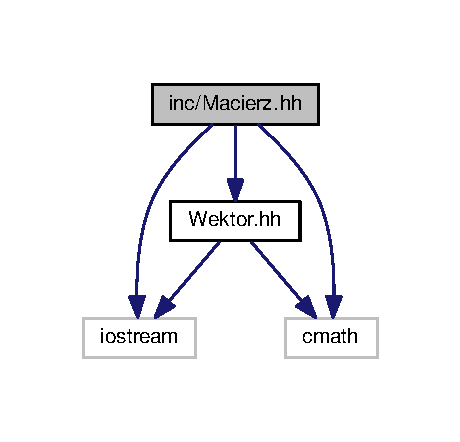
\includegraphics[width=221pt]{Macierz_8hh__incl}
\end{center}
\end{figure}
This graph shows which files directly or indirectly include this file\+:\nopagebreak
\begin{figure}[H]
\begin{center}
\leavevmode
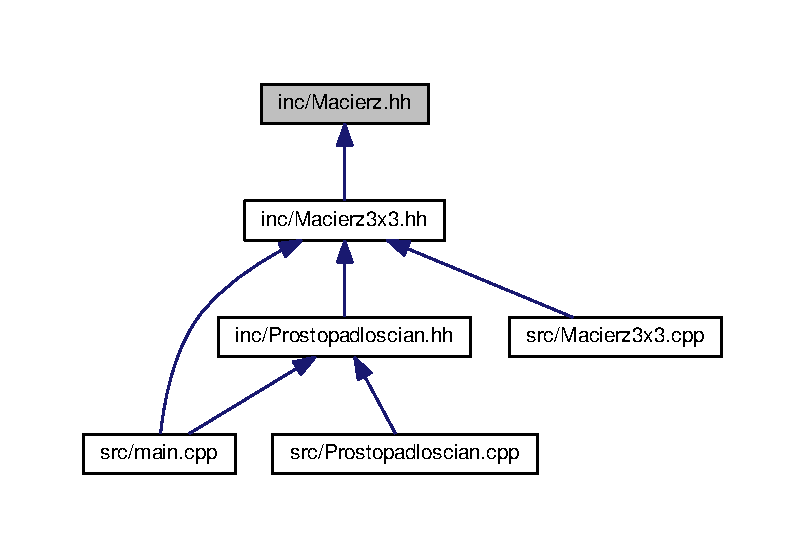
\includegraphics[width=350pt]{Macierz_8hh__dep__incl}
\end{center}
\end{figure}
\subsection*{Classes}
\begin{DoxyCompactItemize}
\item 
class \hyperlink{classMacierz}{Macierz$<$ Wymiar $>$}
\begin{DoxyCompactList}\small\item\em Szablon klasy macierz Szablon klasy macierz jest reprezentacja macierzy w przestrzeni n-\/ wymiarowej gdzie n jest reprezenowana przez argument szablonu wymiar. \end{DoxyCompactList}\end{DoxyCompactItemize}
\subsection*{Functions}
\begin{DoxyCompactItemize}
\item 
\mbox{\Hypertarget{Macierz_8hh_ac3a210e69b75f6e7fe48a36a48982ddc}\label{Macierz_8hh_ac3a210e69b75f6e7fe48a36a48982ddc}} 
{\footnotesize template$<$int Wymiar$>$ }\\std\+::ostream \& {\bfseries operator$<$$<$} (std\+::ostream \&Strm, const \hyperlink{classMacierz}{Macierz}$<$ Wymiar $>$ \&Mac)
\end{DoxyCompactItemize}


\subsection{Detailed Description}
Ten plik zawiera definicję szablonu Macierz$<$$>$ 

Przeciążenie operatora przesuniecia bitowego w lewo sluzy do przekazania strumienia danych na podane wyjscie.


\begin{DoxyParams}[1]{Parameters}
\mbox{\tt in}  & {\em Strm} & -\/ strumień wyjścia \\
\hline
\mbox{\tt in}  & {\em Mac} & -\/ macierz do wyświetlenia \\
\hline
\end{DoxyParams}
\begin{DoxyReturn}{Returns}
strumień wyjścia 
\end{DoxyReturn}

\hypertarget{Macierz3x3_8hh}{}\section{inc/\+Macierz3x3.hh File Reference}
\label{Macierz3x3_8hh}\index{inc/\+Macierz3x3.\+hh@{inc/\+Macierz3x3.\+hh}}


Klasa Macierz3x3 jest instancją szablonu Macierz$<$3$>$ modeluje ona macierz o rozmiarze 3 co powoduje wygenerowanie na podstawie szablonu klasy o wymiarze wiersz/kolumna o rozmiarze 3.  


{\ttfamily \#include $<$iostream$>$}\newline
{\ttfamily \#include \char`\"{}Macierz.\+hh\char`\"{}}\newline
Include dependency graph for Macierz3x3.\+hh\+:\nopagebreak
\begin{figure}[H]
\begin{center}
\leavevmode
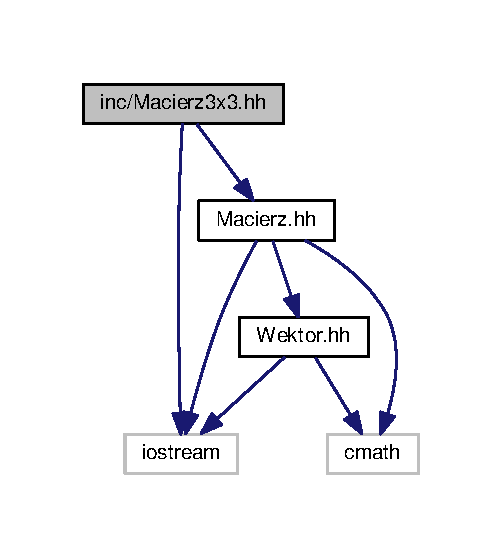
\includegraphics[width=241pt]{Macierz3x3_8hh__incl}
\end{center}
\end{figure}
This graph shows which files directly or indirectly include this file\+:\nopagebreak
\begin{figure}[H]
\begin{center}
\leavevmode
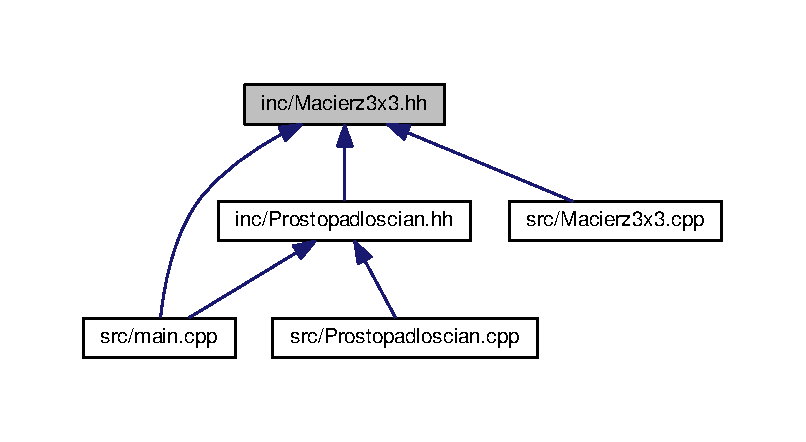
\includegraphics[width=350pt]{Macierz3x3_8hh__dep__incl}
\end{center}
\end{figure}
\subsection*{Typedefs}
\begin{DoxyCompactItemize}
\item 
\mbox{\Hypertarget{Macierz3x3_8hh_ad4fc7b0e263d9a99ba6174f68b52ea87}\label{Macierz3x3_8hh_ad4fc7b0e263d9a99ba6174f68b52ea87}} 
typedef \hyperlink{classMacierz}{Macierz}$<$ 3 $>$ {\bfseries Macierz3x3}
\end{DoxyCompactItemize}
\subsection*{Functions}
\begin{DoxyCompactItemize}
\item 
void \hyperlink{Macierz3x3_8hh_a28670d7aba1ee76534fe5762b3b747b6}{Wylicz\+\_\+macierz\+\_\+x} (\hyperlink{classMacierz}{Macierz3x3} \&Mac)
\begin{DoxyCompactList}\small\item\em Funkcja Wylicz\+\_\+macierz\+\_\+x sluzy do okreslenia wartosci macierzy funkcji trygonometrycznej dla obrotu wokol osi x. \end{DoxyCompactList}\item 
void \hyperlink{Macierz3x3_8hh_aaf1ca1069eac4e0e1d9b093a31ea5003}{Wylicz\+\_\+macierz\+\_\+y} (\hyperlink{classMacierz}{Macierz3x3} \&Mac)
\begin{DoxyCompactList}\small\item\em Funkcja Wylicz\+\_\+macierz\+\_\+y sluzy do okreslenia wartosci macierzy funkcji trygonometrycznej dla obrotu wokol osi y. \end{DoxyCompactList}\item 
void \hyperlink{Macierz3x3_8hh_ab551a0498128eb4b007c4243e9840a40}{Wylicz\+\_\+macierz\+\_\+z} (\hyperlink{classMacierz}{Macierz3x3} \&Mac)
\begin{DoxyCompactList}\small\item\em Funkcja Wylicz\+\_\+macierz\+\_\+z sluzy do okreslenia wartosci macierzy funkcji trygonometrycznej dla obrotu wokol osi z. \end{DoxyCompactList}\end{DoxyCompactItemize}


\subsection{Detailed Description}
Klasa Macierz3x3 jest instancją szablonu Macierz$<$3$>$ modeluje ona macierz o rozmiarze 3 co powoduje wygenerowanie na podstawie szablonu klasy o wymiarze wiersz/kolumna o rozmiarze 3. 



\subsection{Function Documentation}
\mbox{\Hypertarget{Macierz3x3_8hh_a28670d7aba1ee76534fe5762b3b747b6}\label{Macierz3x3_8hh_a28670d7aba1ee76534fe5762b3b747b6}} 
\index{Macierz3x3.\+hh@{Macierz3x3.\+hh}!Wylicz\+\_\+macierz\+\_\+x@{Wylicz\+\_\+macierz\+\_\+x}}
\index{Wylicz\+\_\+macierz\+\_\+x@{Wylicz\+\_\+macierz\+\_\+x}!Macierz3x3.\+hh@{Macierz3x3.\+hh}}
\subsubsection{\texorpdfstring{Wylicz\+\_\+macierz\+\_\+x()}{Wylicz\_macierz\_x()}}
{\footnotesize\ttfamily void Wylicz\+\_\+macierz\+\_\+x (\begin{DoxyParamCaption}\item[{\hyperlink{classMacierz}{Macierz3x3} \&}]{Mac }\end{DoxyParamCaption})}



Funkcja Wylicz\+\_\+macierz\+\_\+x sluzy do okreslenia wartosci macierzy funkcji trygonometrycznej dla obrotu wokol osi x. 


\begin{DoxyParams}[1]{Parameters}
\mbox{\tt in}  & {\em Mac} & -\/ oryginalna macierz sluzaca do przechowywania wartosci obrotu\\
\hline
\end{DoxyParams}
Funkcja Wylicz\+\_\+macierz\+\_\+x sluzy do okreslenia wartosci macierzy funkcji trygonometrycznej dla obrotu wokol osi x. \mbox{\Hypertarget{Macierz3x3_8hh_aaf1ca1069eac4e0e1d9b093a31ea5003}\label{Macierz3x3_8hh_aaf1ca1069eac4e0e1d9b093a31ea5003}} 
\index{Macierz3x3.\+hh@{Macierz3x3.\+hh}!Wylicz\+\_\+macierz\+\_\+y@{Wylicz\+\_\+macierz\+\_\+y}}
\index{Wylicz\+\_\+macierz\+\_\+y@{Wylicz\+\_\+macierz\+\_\+y}!Macierz3x3.\+hh@{Macierz3x3.\+hh}}
\subsubsection{\texorpdfstring{Wylicz\+\_\+macierz\+\_\+y()}{Wylicz\_macierz\_y()}}
{\footnotesize\ttfamily void Wylicz\+\_\+macierz\+\_\+y (\begin{DoxyParamCaption}\item[{\hyperlink{classMacierz}{Macierz3x3} \&}]{Mac }\end{DoxyParamCaption})}



Funkcja Wylicz\+\_\+macierz\+\_\+y sluzy do okreslenia wartosci macierzy funkcji trygonometrycznej dla obrotu wokol osi y. 


\begin{DoxyParams}[1]{Parameters}
\mbox{\tt in}  & {\em Mac} & -\/ oryginalna macierz sluzaca do przechowywania wartosci obrotu\\
\hline
\end{DoxyParams}
Funkcja Wylicz\+\_\+macierz\+\_\+y sluzy do okreslenia wartosci macierzy funkcji trygonometrycznej dla obrotu wokol osi y. \mbox{\Hypertarget{Macierz3x3_8hh_ab551a0498128eb4b007c4243e9840a40}\label{Macierz3x3_8hh_ab551a0498128eb4b007c4243e9840a40}} 
\index{Macierz3x3.\+hh@{Macierz3x3.\+hh}!Wylicz\+\_\+macierz\+\_\+z@{Wylicz\+\_\+macierz\+\_\+z}}
\index{Wylicz\+\_\+macierz\+\_\+z@{Wylicz\+\_\+macierz\+\_\+z}!Macierz3x3.\+hh@{Macierz3x3.\+hh}}
\subsubsection{\texorpdfstring{Wylicz\+\_\+macierz\+\_\+z()}{Wylicz\_macierz\_z()}}
{\footnotesize\ttfamily void Wylicz\+\_\+macierz\+\_\+z (\begin{DoxyParamCaption}\item[{\hyperlink{classMacierz}{Macierz3x3} \&}]{Mac }\end{DoxyParamCaption})}



Funkcja Wylicz\+\_\+macierz\+\_\+z sluzy do okreslenia wartosci macierzy funkcji trygonometrycznej dla obrotu wokol osi z. 


\begin{DoxyParams}[1]{Parameters}
\mbox{\tt in}  & {\em Mac} & -\/ oryginalna macierz sluzaca do przechowywania wartosci obrotu\\
\hline
\end{DoxyParams}
Funkcja Wylicz\+\_\+macierz\+\_\+z sluzy do okreslenia wartosci macierzy funkcji trygonometrycznej dla obrotu wokol osi z. 
\hypertarget{Prostopadloscian_8hh}{}\section{inc/\+Prostopadloscian.hh File Reference}
\label{Prostopadloscian_8hh}\index{inc/\+Prostopadloscian.\+hh@{inc/\+Prostopadloscian.\+hh}}


Ten plik zawiera definicję Klasy.  


{\ttfamily \#include $<$iostream$>$}\newline
{\ttfamily \#include $<$fstream$>$}\newline
{\ttfamily \#include \char`\"{}Wektor3\+D.\+hh\char`\"{}}\newline
{\ttfamily \#include \char`\"{}Macierz3x3.\+hh\char`\"{}}\newline
Include dependency graph for Prostopadloscian.\+hh\+:\nopagebreak
\begin{figure}[H]
\begin{center}
\leavevmode
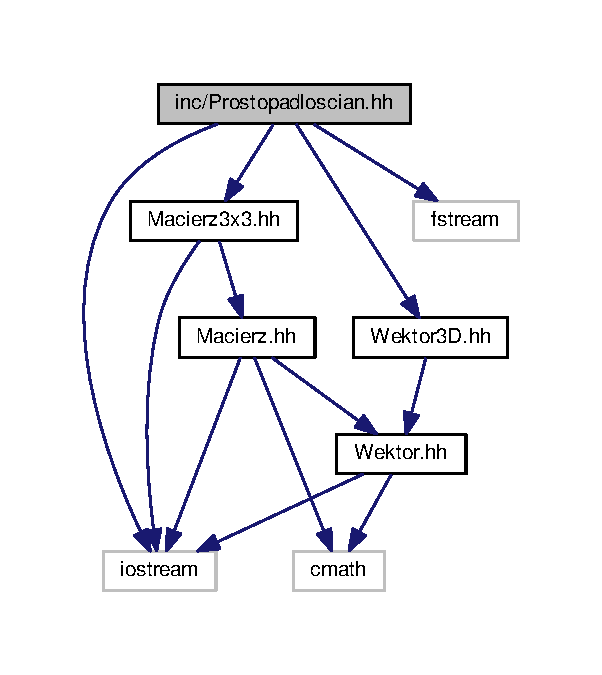
\includegraphics[width=289pt]{Prostopadloscian_8hh__incl}
\end{center}
\end{figure}
This graph shows which files directly or indirectly include this file\+:\nopagebreak
\begin{figure}[H]
\begin{center}
\leavevmode
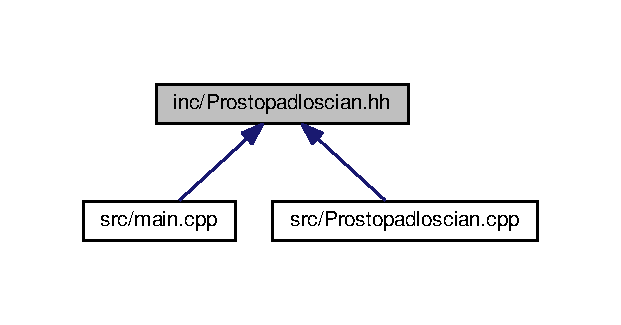
\includegraphics[width=298pt]{Prostopadloscian_8hh__dep__incl}
\end{center}
\end{figure}
\subsection*{Classes}
\begin{DoxyCompactItemize}
\item 
class \hyperlink{classProstopadloscian}{Prostopadloscian}
\begin{DoxyCompactList}\small\item\em Klasa prostopadloscian Klasa prostopadloscian jest reprezentacja prostopadloscianu w przestrzeni 3D. \end{DoxyCompactList}\end{DoxyCompactItemize}
\subsection*{Macros}
\begin{DoxyCompactItemize}
\item 
\mbox{\Hypertarget{Prostopadloscian_8hh_a6ebf6899d6c1c8b7b9d09be872c05aae}\label{Prostopadloscian_8hh_a6ebf6899d6c1c8b7b9d09be872c05aae}} 
\#define {\bfseries E\+PS}~0.\+00000000000001
\end{DoxyCompactItemize}
\subsection*{Functions}
\begin{DoxyCompactItemize}
\item 
std\+::ostream \& \hyperlink{Prostopadloscian_8hh_a0a77f9bb1cc3f07e11031b947e6e7322}{operator$<$$<$} (std\+::ostream \&Strm, const \hyperlink{classProstopadloscian}{Prostopadloscian} \&Pr)
\begin{DoxyCompactList}\small\item\em Przeciążenie operatora przesuniecia bitowego w lewo sluzy do przekazania strumienia danych na podane wyjscie. \end{DoxyCompactList}\item 
void \hyperlink{Prostopadloscian_8hh_a42155017ae1f49acb330164b11df2b97}{Zapis\+Do\+Strumienia} (ostream \&Strm\+Wy, \hyperlink{classMacierz}{Macierz3x3} Przesuniecie, \hyperlink{classProstopadloscian}{Prostopadloscian} \&Pr)
\begin{DoxyCompactList}\small\item\em Zapis danych do strumienia. \end{DoxyCompactList}\item 
void \hyperlink{Prostopadloscian_8hh_a1fd5a38f6b20a1ea903c1ec882222dd6}{Zapis\+Do\+Strumienia} (ostream \&Strm\+Wy, \hyperlink{classWektor}{Wektor3D} Przesuniecie, \hyperlink{classProstopadloscian}{Prostopadloscian} \&Pr)
\begin{DoxyCompactList}\small\item\em Zapis danych do strumienia. \end{DoxyCompactList}\item 
bool \hyperlink{Prostopadloscian_8hh_a7b6b375f9857993a4457fc37f47d585d}{Zapis\+Wspolrzednych\+Do\+Pliku} (const char $\ast$s\+Nazwa\+Pliku, \hyperlink{classMacierz}{Macierz3x3} Przesuniecie, \hyperlink{classProstopadloscian}{Prostopadloscian} \&Pr)
\begin{DoxyCompactList}\small\item\em Zapis danych do pliku. \end{DoxyCompactList}\item 
bool \hyperlink{Prostopadloscian_8hh_a140b1afdfa25067b9e9fcd7a738af090}{Zapis\+Wspolrzednych\+Do\+Pliku} (const char $\ast$s\+Nazwa\+Pliku, \hyperlink{classWektor}{Wektor3D} Przesuniecie, \hyperlink{classProstopadloscian}{Prostopadloscian} \&Pr)
\begin{DoxyCompactList}\small\item\em Zapis danych do pliku. \end{DoxyCompactList}\end{DoxyCompactItemize}


\subsection{Detailed Description}
Ten plik zawiera definicję Klasy. 



\subsection{Function Documentation}
\mbox{\Hypertarget{Prostopadloscian_8hh_a0a77f9bb1cc3f07e11031b947e6e7322}\label{Prostopadloscian_8hh_a0a77f9bb1cc3f07e11031b947e6e7322}} 
\index{Prostopadloscian.\+hh@{Prostopadloscian.\+hh}!operator$<$$<$@{operator$<$$<$}}
\index{operator$<$$<$@{operator$<$$<$}!Prostopadloscian.\+hh@{Prostopadloscian.\+hh}}
\subsubsection{\texorpdfstring{operator$<$$<$()}{operator<<()}}
{\footnotesize\ttfamily std\+::ostream\& operator$<$$<$ (\begin{DoxyParamCaption}\item[{std\+::ostream \&}]{Strm,  }\item[{const \hyperlink{classProstopadloscian}{Prostopadloscian} \&}]{Pr }\end{DoxyParamCaption})}



Przeciążenie operatora przesuniecia bitowego w lewo sluzy do przekazania strumienia danych na podane wyjscie. 


\begin{DoxyParams}[1]{Parameters}
\mbox{\tt in}  & {\em Strm} & -\/ strumień wyjścia \\
\hline
\mbox{\tt in}  & {\em Pr} & -\/ prostopadloscian do wyświetlenia \\
\hline
\end{DoxyParams}
\begin{DoxyReturn}{Returns}
strumień wyjścia
\end{DoxyReturn}
Przeciążenie operatora przesuniecia bitowego w lewo sluzy do przekazania strumienia danych na podane wyjscie. \mbox{\Hypertarget{Prostopadloscian_8hh_a42155017ae1f49acb330164b11df2b97}\label{Prostopadloscian_8hh_a42155017ae1f49acb330164b11df2b97}} 
\index{Prostopadloscian.\+hh@{Prostopadloscian.\+hh}!Zapis\+Do\+Strumienia@{Zapis\+Do\+Strumienia}}
\index{Zapis\+Do\+Strumienia@{Zapis\+Do\+Strumienia}!Prostopadloscian.\+hh@{Prostopadloscian.\+hh}}
\subsubsection{\texorpdfstring{Zapis\+Do\+Strumienia()}{ZapisDoStrumienia()}\hspace{0.1cm}{\footnotesize\ttfamily [1/2]}}
{\footnotesize\ttfamily void Zapis\+Do\+Strumienia (\begin{DoxyParamCaption}\item[{ostream \&}]{Strm\+Wy,  }\item[{\hyperlink{classMacierz}{Macierz3x3}}]{Przesuniecie,  }\item[{\hyperlink{classProstopadloscian}{Prostopadloscian} \&}]{Pr }\end{DoxyParamCaption})}



Zapis danych do strumienia. 

Zapis wspolrzednych zbioru punktow do strumienia wyjściowego. Dane sa odpowiednio sformatowane, tzn. przyjęto notację stałoprzecinkową z dokładnością do 10 miejsca po przecinku. Szerokość wyświetlanego pola to 16 miejsc, sposób wyrównywania -\/ do prawej strony. 
\begin{DoxyParams}[1]{Parameters}
\mbox{\tt in}  & {\em Strm\+Wy} & -\/ strumien wyjsciowy, do ktorego maja zostac zapisane kolejne wspolrzedne. \\
\hline
\mbox{\tt in}  & {\em Przesuniecie} & -\/ ten parameter jest aby przekazac macierz obrotu \\
\hline
\mbox{\tt in}  & {\em \hyperlink{classProstopadloscian}{Prostopadloscian}} & -\/ ten parameter przekazuje oryginal obiektu bryly \\
\hline
\end{DoxyParams}
\mbox{\Hypertarget{Prostopadloscian_8hh_a1fd5a38f6b20a1ea903c1ec882222dd6}\label{Prostopadloscian_8hh_a1fd5a38f6b20a1ea903c1ec882222dd6}} 
\index{Prostopadloscian.\+hh@{Prostopadloscian.\+hh}!Zapis\+Do\+Strumienia@{Zapis\+Do\+Strumienia}}
\index{Zapis\+Do\+Strumienia@{Zapis\+Do\+Strumienia}!Prostopadloscian.\+hh@{Prostopadloscian.\+hh}}
\subsubsection{\texorpdfstring{Zapis\+Do\+Strumienia()}{ZapisDoStrumienia()}\hspace{0.1cm}{\footnotesize\ttfamily [2/2]}}
{\footnotesize\ttfamily void Zapis\+Do\+Strumienia (\begin{DoxyParamCaption}\item[{ostream \&}]{Strm\+Wy,  }\item[{\hyperlink{classWektor}{Wektor3D}}]{Przesuniecie,  }\item[{\hyperlink{classProstopadloscian}{Prostopadloscian} \&}]{Pr }\end{DoxyParamCaption})}



Zapis danych do strumienia. 

Zapis wspolrzednych zbioru punktow do strumienia wyjściowego. Dane sa odpowiednio sformatowane, tzn. przyjęto notację stałoprzecinkową z dokładnością do 10 miejsca po przecinku. Szerokość wyświetlanego pola to 16 miejsc, sposób wyrównywania -\/ do prawej strony. 
\begin{DoxyParams}[1]{Parameters}
\mbox{\tt in}  & {\em Strm\+Wy} & -\/ strumien wyjsciowy, do ktorego maja zostac zapisane kolejne wspolrzedne. \\
\hline
\mbox{\tt in}  & {\em Przesuniecie} & -\/ ten parameter jest aby przekazac wektor przesuniecia \\
\hline
\mbox{\tt in}  & {\em \hyperlink{classProstopadloscian}{Prostopadloscian}} & -\/ ten parameter przekazuje oryginal obiektu bryly \\
\hline
\end{DoxyParams}
\mbox{\Hypertarget{Prostopadloscian_8hh_a7b6b375f9857993a4457fc37f47d585d}\label{Prostopadloscian_8hh_a7b6b375f9857993a4457fc37f47d585d}} 
\index{Prostopadloscian.\+hh@{Prostopadloscian.\+hh}!Zapis\+Wspolrzednych\+Do\+Pliku@{Zapis\+Wspolrzednych\+Do\+Pliku}}
\index{Zapis\+Wspolrzednych\+Do\+Pliku@{Zapis\+Wspolrzednych\+Do\+Pliku}!Prostopadloscian.\+hh@{Prostopadloscian.\+hh}}
\subsubsection{\texorpdfstring{Zapis\+Wspolrzednych\+Do\+Pliku()}{ZapisWspolrzednychDoPliku()}\hspace{0.1cm}{\footnotesize\ttfamily [1/2]}}
{\footnotesize\ttfamily bool Zapis\+Wspolrzednych\+Do\+Pliku (\begin{DoxyParamCaption}\item[{const char $\ast$}]{s\+Nazwa\+Pliku,  }\item[{\hyperlink{classMacierz}{Macierz3x3}}]{Przesuniecie,  }\item[{\hyperlink{classProstopadloscian}{Prostopadloscian} \&}]{Pr }\end{DoxyParamCaption})}



Zapis danych do pliku. 

Zapis wspolrzednych zbioru punktow do pliku, z ktorego dane odczyta program gnuplot i narysuje je w swoim oknie graficznym. 
\begin{DoxyParams}[1]{Parameters}
\mbox{\tt in}  & {\em s\+Nazwa\+Pliku} & -\/ nazwa pliku, do którego zostana zapisane wspolrzędne punktów. \\
\hline
\mbox{\tt in}  & {\em Przesuniecie} & -\/ ten parameter jest aby przekazac macierz obrotu \\
\hline
\mbox{\tt in}  & {\em \hyperlink{classProstopadloscian}{Prostopadloscian}} & -\/ ten parameter przekazuje oryginal obiektu bryly \\
\hline
\end{DoxyParams}

\begin{DoxyRetVals}{Return values}
{\em true} & -\/ gdy operacja zapisu powiodła się, \\
\hline
{\em false} & -\/ w przypadku przeciwnym. \\
\hline
\end{DoxyRetVals}
\mbox{\Hypertarget{Prostopadloscian_8hh_a140b1afdfa25067b9e9fcd7a738af090}\label{Prostopadloscian_8hh_a140b1afdfa25067b9e9fcd7a738af090}} 
\index{Prostopadloscian.\+hh@{Prostopadloscian.\+hh}!Zapis\+Wspolrzednych\+Do\+Pliku@{Zapis\+Wspolrzednych\+Do\+Pliku}}
\index{Zapis\+Wspolrzednych\+Do\+Pliku@{Zapis\+Wspolrzednych\+Do\+Pliku}!Prostopadloscian.\+hh@{Prostopadloscian.\+hh}}
\subsubsection{\texorpdfstring{Zapis\+Wspolrzednych\+Do\+Pliku()}{ZapisWspolrzednychDoPliku()}\hspace{0.1cm}{\footnotesize\ttfamily [2/2]}}
{\footnotesize\ttfamily bool Zapis\+Wspolrzednych\+Do\+Pliku (\begin{DoxyParamCaption}\item[{const char $\ast$}]{s\+Nazwa\+Pliku,  }\item[{\hyperlink{classWektor}{Wektor3D}}]{Przesuniecie,  }\item[{\hyperlink{classProstopadloscian}{Prostopadloscian} \&}]{Pr }\end{DoxyParamCaption})}



Zapis danych do pliku. 

Zapis wspolrzednych zbioru punktow do pliku, z ktorego dane odczyta program gnuplot i narysuje je w swoim oknie graficznym. 
\begin{DoxyParams}[1]{Parameters}
\mbox{\tt in}  & {\em s\+Nazwa\+Pliku} & -\/ nazwa pliku, do którego zostana zapisane wspolrzędne punktów. \\
\hline
\mbox{\tt in}  & {\em Przesuniecie} & -\/ ten parameter jest aby przekazac wektor przesuniecia \\
\hline
\mbox{\tt in}  & {\em \hyperlink{classProstopadloscian}{Prostopadloscian}} & -\/ ten parameter przekazuje oryginal obiektu bryly \\
\hline
\end{DoxyParams}

\begin{DoxyRetVals}{Return values}
{\em true} & -\/ gdy operacja zapisu powiodła się, \\
\hline
{\em false} & -\/ w przypadku przeciwnym. \\
\hline
\end{DoxyRetVals}

\hypertarget{Wektor_8hh}{}\section{inc/\+Wektor.hh File Reference}
\label{Wektor_8hh}\index{inc/\+Wektor.\+hh@{inc/\+Wektor.\+hh}}


Ten plik zawiera definicję szablonu Wektor$<$$>$  


{\ttfamily \#include $<$iostream$>$}\newline
{\ttfamily \#include $<$cmath$>$}\newline
Include dependency graph for Wektor.\+hh\+:\nopagebreak
\begin{figure}[H]
\begin{center}
\leavevmode
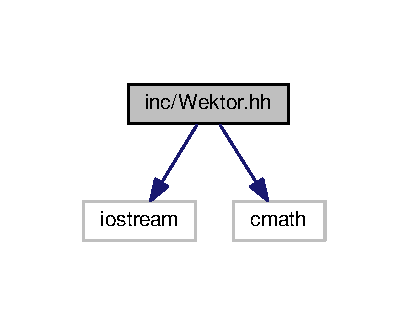
\includegraphics[width=196pt]{Wektor_8hh__incl}
\end{center}
\end{figure}
This graph shows which files directly or indirectly include this file\+:\nopagebreak
\begin{figure}[H]
\begin{center}
\leavevmode
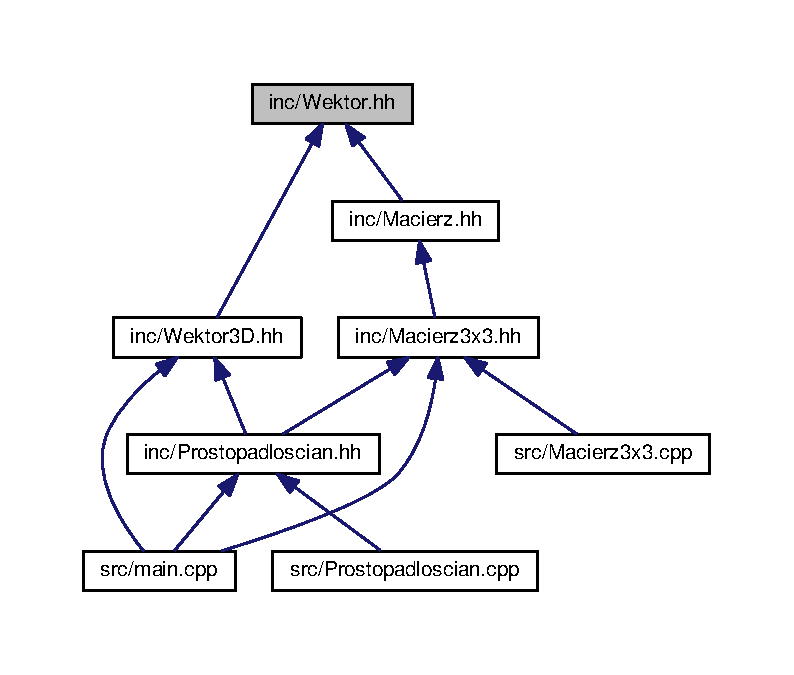
\includegraphics[width=350pt]{Wektor_8hh__dep__incl}
\end{center}
\end{figure}
\subsection*{Classes}
\begin{DoxyCompactItemize}
\item 
class \hyperlink{classWektor}{Wektor$<$ Wymiar $>$}
\begin{DoxyCompactList}\small\item\em Szablon klasy wektor Szablon klasy wektor jest reprezentacja wektoru w przestrzeni n-\/ wymiarowej gdzie n jest reprezenowana przez argument szablonu wymiar. \end{DoxyCompactList}\end{DoxyCompactItemize}
\subsection*{Functions}
\begin{DoxyCompactItemize}
\item 
{\footnotesize template$<$int Wymiar$>$ }\\std\+::istream \& \hyperlink{Wektor_8hh_a936d42e42728823fb375e5e2122c2fe0}{operator$>$$>$} (std\+::istream \&Strm, \hyperlink{classWektor}{Wektor}$<$ Wymiar $>$ \&Wek)
\begin{DoxyCompactList}\small\item\em Przeciążenie operatora przesuniecia bitowego w prawo sluzy do przekazania strumienia danych na podane wejscie. \end{DoxyCompactList}\item 
{\footnotesize template$<$int Wymiar$>$ }\\std\+::ostream \& \hyperlink{Wektor_8hh_a15a4e77c646218f10d5e34a3fd4a877a}{operator$<$$<$} (std\+::ostream \&Strm, const \hyperlink{classWektor}{Wektor}$<$ Wymiar $>$ \&Wek)
\begin{DoxyCompactList}\small\item\em Przeciążenie operatora przesuniecia bitowego w lewo sluzy do przekazania strumienia danych na podane wyjscie. \end{DoxyCompactList}\end{DoxyCompactItemize}


\subsection{Detailed Description}
Ten plik zawiera definicję szablonu Wektor$<$$>$ 



\subsection{Function Documentation}
\mbox{\Hypertarget{Wektor_8hh_a15a4e77c646218f10d5e34a3fd4a877a}\label{Wektor_8hh_a15a4e77c646218f10d5e34a3fd4a877a}} 
\index{Wektor.\+hh@{Wektor.\+hh}!operator$<$$<$@{operator$<$$<$}}
\index{operator$<$$<$@{operator$<$$<$}!Wektor.\+hh@{Wektor.\+hh}}
\subsubsection{\texorpdfstring{operator$<$$<$()}{operator<<()}}
{\footnotesize\ttfamily template$<$int Wymiar$>$ \\
std\+::ostream\& operator$<$$<$ (\begin{DoxyParamCaption}\item[{std\+::ostream \&}]{Strm,  }\item[{const \hyperlink{classWektor}{Wektor}$<$ Wymiar $>$ \&}]{Wek }\end{DoxyParamCaption})\hspace{0.3cm}{\ttfamily [inline]}}



Przeciążenie operatora przesuniecia bitowego w lewo sluzy do przekazania strumienia danych na podane wyjscie. 


\begin{DoxyParams}[1]{Parameters}
\mbox{\tt in}  & {\em Strm} & -\/ strumień wyjścia \\
\hline
\mbox{\tt in}  & {\em Wek} & -\/ wektor do wyświetlenia \\
\hline
\end{DoxyParams}
\begin{DoxyReturn}{Returns}
strumień wyjścia 
\end{DoxyReturn}
\mbox{\Hypertarget{Wektor_8hh_a936d42e42728823fb375e5e2122c2fe0}\label{Wektor_8hh_a936d42e42728823fb375e5e2122c2fe0}} 
\index{Wektor.\+hh@{Wektor.\+hh}!operator$>$$>$@{operator$>$$>$}}
\index{operator$>$$>$@{operator$>$$>$}!Wektor.\+hh@{Wektor.\+hh}}
\subsubsection{\texorpdfstring{operator$>$$>$()}{operator>>()}}
{\footnotesize\ttfamily template$<$int Wymiar$>$ \\
std\+::istream\& operator$>$$>$ (\begin{DoxyParamCaption}\item[{std\+::istream \&}]{Strm,  }\item[{\hyperlink{classWektor}{Wektor}$<$ Wymiar $>$ \&}]{Wek }\end{DoxyParamCaption})\hspace{0.3cm}{\ttfamily [inline]}}



Przeciążenie operatora przesuniecia bitowego w prawo sluzy do przekazania strumienia danych na podane wejscie. 


\begin{DoxyParams}[1]{Parameters}
\mbox{\tt in}  & {\em Strm} & -\/ strumień wejscia \\
\hline
\mbox{\tt in}  & {\em Wek} & -\/ wektor do wprowadzenia \\
\hline
\end{DoxyParams}
\begin{DoxyReturn}{Returns}
strumień wejscia 
\end{DoxyReturn}

\hypertarget{Wektor3D_8hh}{}\section{inc/\+Wektor3D.hh File Reference}
\label{Wektor3D_8hh}\index{inc/\+Wektor3\+D.\+hh@{inc/\+Wektor3\+D.\+hh}}


Klasa Wektor3D jest instancją szablonu \hyperlink{classWektor}{Wektor$<$3$>$} modeluje ona wektor o rozmiarze 3 co powoduje wygenerowanie na podstawie szablonu klasy o wymiarze 3.  


{\ttfamily \#include \char`\"{}Wektor.\+hh\char`\"{}}\newline
Include dependency graph for Wektor3\+D.\+hh\+:\nopagebreak
\begin{figure}[H]
\begin{center}
\leavevmode
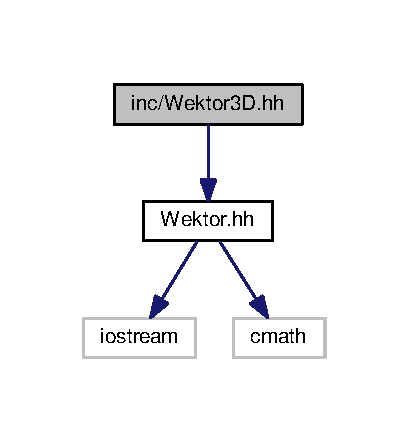
\includegraphics[width=196pt]{Wektor3D_8hh__incl}
\end{center}
\end{figure}
This graph shows which files directly or indirectly include this file\+:\nopagebreak
\begin{figure}[H]
\begin{center}
\leavevmode
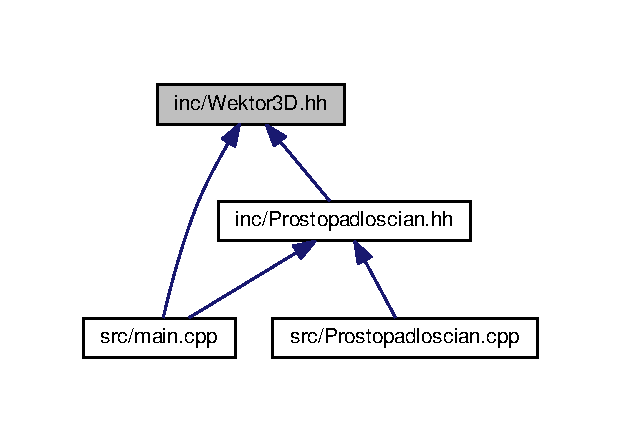
\includegraphics[width=298pt]{Wektor3D_8hh__dep__incl}
\end{center}
\end{figure}
\subsection*{Typedefs}
\begin{DoxyCompactItemize}
\item 
\mbox{\Hypertarget{Wektor3D_8hh_ac353a272b38b4ad342f7181ad7bdb91a}\label{Wektor3D_8hh_ac353a272b38b4ad342f7181ad7bdb91a}} 
typedef \hyperlink{classWektor}{Wektor}$<$ 3 $>$ {\bfseries Wektor3D}
\end{DoxyCompactItemize}


\subsection{Detailed Description}
Klasa Wektor3D jest instancją szablonu \hyperlink{classWektor}{Wektor$<$3$>$} modeluje ona wektor o rozmiarze 3 co powoduje wygenerowanie na podstawie szablonu klasy o wymiarze 3. 


\hypertarget{lacze__do__gnuplota_8cpp}{}\section{src/lacze\+\_\+do\+\_\+gnuplota.cpp File Reference}
\label{lacze__do__gnuplota_8cpp}\index{src/lacze\+\_\+do\+\_\+gnuplota.\+cpp@{src/lacze\+\_\+do\+\_\+gnuplota.\+cpp}}


Plik lacze do gnuplota Plik ten umożliwia wyświetlenie prostopadłościaniu w programie gnuplot.  


{\ttfamily \#include $<$cstdlib$>$}\newline
{\ttfamily \#include $<$cstdio$>$}\newline
{\ttfamily \#include $<$cstring$>$}\newline
{\ttfamily \#include $<$cmath$>$}\newline
{\ttfamily \#include $<$iostream$>$}\newline
{\ttfamily \#include $<$sys/stat.\+h$>$}\newline
{\ttfamily \#include $<$unistd.\+h$>$}\newline
{\ttfamily \#include $<$fcntl.\+h$>$}\newline
{\ttfamily \#include $<$sstream$>$}\newline
{\ttfamily \#include \char`\"{}lacze\+\_\+do\+\_\+gnuplota.\+hh\char`\"{}}\newline
Include dependency graph for lacze\+\_\+do\+\_\+gnuplota.\+cpp\+:\nopagebreak
\begin{figure}[H]
\begin{center}
\leavevmode
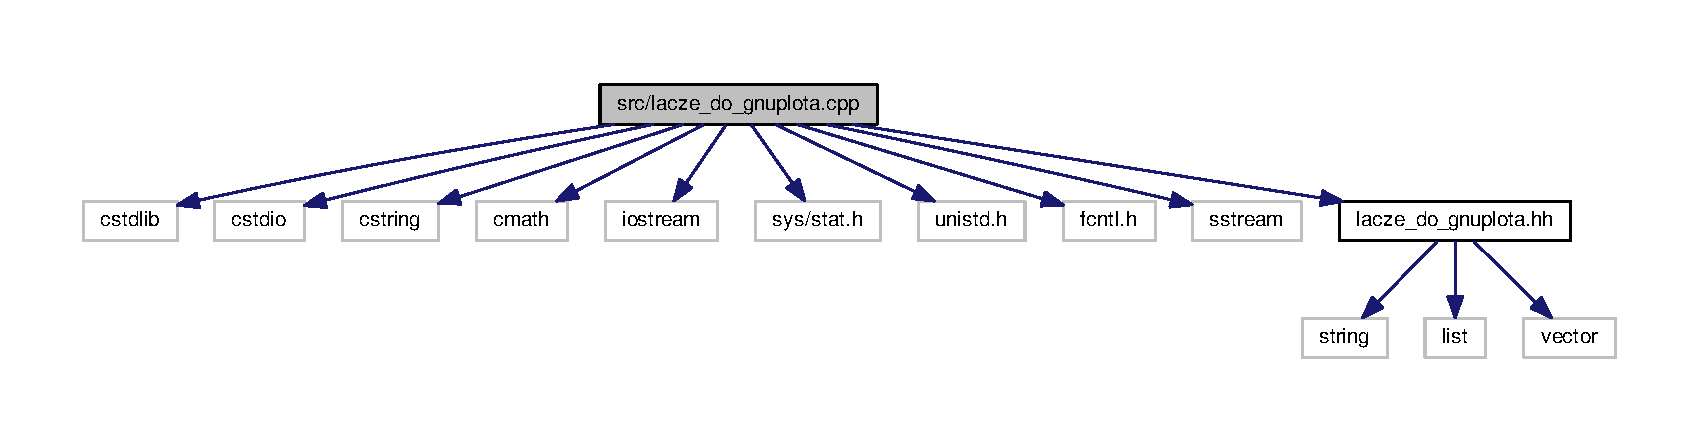
\includegraphics[width=350pt]{lacze__do__gnuplota_8cpp__incl}
\end{center}
\end{figure}
\subsection*{Namespaces}
\begin{DoxyCompactItemize}
\item 
 \hyperlink{namespacePzG}{PzG}
\begin{DoxyCompactList}\small\item\em Moduł narzędzi umożliwiających połącznie z G\+N\+U\+Plotem. \end{DoxyCompactList}\end{DoxyCompactItemize}
\subsection*{Macros}
\begin{DoxyCompactItemize}
\item 
\mbox{\Hypertarget{lacze__do__gnuplota_8cpp_ac00bfb46347d26fdc58568fe1ab5fa5b}\label{lacze__do__gnuplota_8cpp_ac00bfb46347d26fdc58568fe1ab5fa5b}} 
\#define {\bfseries S\+T\+D\+IN}~0
\item 
\mbox{\Hypertarget{lacze__do__gnuplota_8cpp_a8875037d0772a4fc34516f1e03d7e238}\label{lacze__do__gnuplota_8cpp_a8875037d0772a4fc34516f1e03d7e238}} 
\#define {\bfseries S\+T\+D\+O\+UT}~1
\item 
\mbox{\Hypertarget{lacze__do__gnuplota_8cpp_a2b501945c8d86114fcf6420cc1ee6306}\label{lacze__do__gnuplota_8cpp_a2b501945c8d86114fcf6420cc1ee6306}} 
\#define {\bfseries R\+O\+Z\+\_\+\+L\+I\+N\+II}~120
\end{DoxyCompactItemize}
\subsection*{Functions}
\begin{DoxyCompactItemize}
\item 
\mbox{\Hypertarget{namespacePzG_ae1ae4d36f66c77879380ba73da8e20e3}\label{namespacePzG_ae1ae4d36f66c77879380ba73da8e20e3}} 
bool {\bfseries Pz\+G\+::\+Czy\+Jest\+Plik} (char const $\ast$Nazwa\+Pliku)
\end{DoxyCompactItemize}


\subsection{Detailed Description}
Plik lacze do gnuplota Plik ten umożliwia wyświetlenie prostopadłościaniu w programie gnuplot. 


\hypertarget{Macierz3x3_8cpp}{}\section{src/\+Macierz3x3.cpp File Reference}
\label{Macierz3x3_8cpp}\index{src/\+Macierz3x3.\+cpp@{src/\+Macierz3x3.\+cpp}}


Plik Macierz3x3 Wylicza macierz obrotu rotacji dla nastepujacych osi x,y i z.  


{\ttfamily \#include \char`\"{}Macierz3x3.\+hh\char`\"{}}\newline
Include dependency graph for Macierz3x3.\+cpp\+:\nopagebreak
\begin{figure}[H]
\begin{center}
\leavevmode
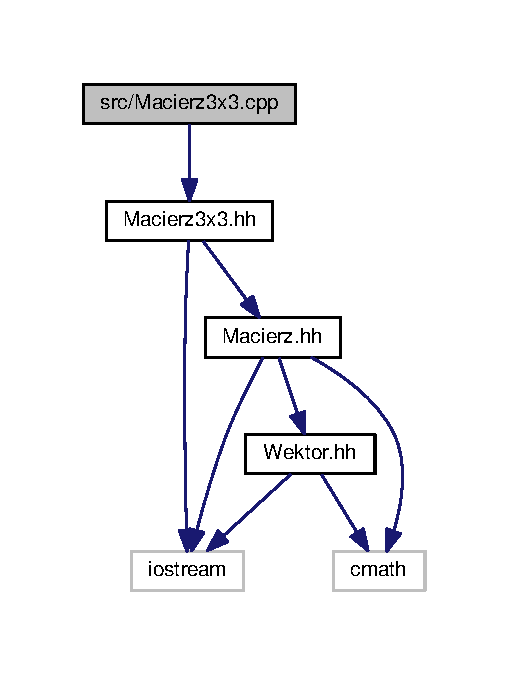
\includegraphics[width=244pt]{Macierz3x3_8cpp__incl}
\end{center}
\end{figure}
\subsection*{Functions}
\begin{DoxyCompactItemize}
\item 
void \hyperlink{Macierz3x3_8cpp_a28670d7aba1ee76534fe5762b3b747b6}{Wylicz\+\_\+macierz\+\_\+x} (\hyperlink{classMacierz}{Macierz3x3} \&Mac)
\begin{DoxyCompactList}\small\item\em \hyperlink{classMacierz}{Macierz} rotacji dla osi x. \end{DoxyCompactList}\item 
void \hyperlink{Macierz3x3_8cpp_aaf1ca1069eac4e0e1d9b093a31ea5003}{Wylicz\+\_\+macierz\+\_\+y} (\hyperlink{classMacierz}{Macierz3x3} \&Mac)
\begin{DoxyCompactList}\small\item\em \hyperlink{classMacierz}{Macierz} rotacji dla osi y. \end{DoxyCompactList}\item 
void \hyperlink{Macierz3x3_8cpp_ab551a0498128eb4b007c4243e9840a40}{Wylicz\+\_\+macierz\+\_\+z} (\hyperlink{classMacierz}{Macierz3x3} \&Mac)
\begin{DoxyCompactList}\small\item\em \hyperlink{classMacierz}{Macierz} rotacji dla osi z. \end{DoxyCompactList}\end{DoxyCompactItemize}


\subsection{Detailed Description}
Plik Macierz3x3 Wylicza macierz obrotu rotacji dla nastepujacych osi x,y i z. 



\subsection{Function Documentation}
\mbox{\Hypertarget{Macierz3x3_8cpp_a28670d7aba1ee76534fe5762b3b747b6}\label{Macierz3x3_8cpp_a28670d7aba1ee76534fe5762b3b747b6}} 
\index{Macierz3x3.\+cpp@{Macierz3x3.\+cpp}!Wylicz\+\_\+macierz\+\_\+x@{Wylicz\+\_\+macierz\+\_\+x}}
\index{Wylicz\+\_\+macierz\+\_\+x@{Wylicz\+\_\+macierz\+\_\+x}!Macierz3x3.\+cpp@{Macierz3x3.\+cpp}}
\subsubsection{\texorpdfstring{Wylicz\+\_\+macierz\+\_\+x()}{Wylicz\_macierz\_x()}}
{\footnotesize\ttfamily void Wylicz\+\_\+macierz\+\_\+x (\begin{DoxyParamCaption}\item[{\hyperlink{classMacierz}{Macierz3x3} \&}]{Mac }\end{DoxyParamCaption})}



\hyperlink{classMacierz}{Macierz} rotacji dla osi x. 

Funkcja Wylicz\+\_\+macierz\+\_\+x sluzy do okreslenia wartosci macierzy funkcji trygonometrycznej dla obrotu wokol osi x. \mbox{\Hypertarget{Macierz3x3_8cpp_aaf1ca1069eac4e0e1d9b093a31ea5003}\label{Macierz3x3_8cpp_aaf1ca1069eac4e0e1d9b093a31ea5003}} 
\index{Macierz3x3.\+cpp@{Macierz3x3.\+cpp}!Wylicz\+\_\+macierz\+\_\+y@{Wylicz\+\_\+macierz\+\_\+y}}
\index{Wylicz\+\_\+macierz\+\_\+y@{Wylicz\+\_\+macierz\+\_\+y}!Macierz3x3.\+cpp@{Macierz3x3.\+cpp}}
\subsubsection{\texorpdfstring{Wylicz\+\_\+macierz\+\_\+y()}{Wylicz\_macierz\_y()}}
{\footnotesize\ttfamily void Wylicz\+\_\+macierz\+\_\+y (\begin{DoxyParamCaption}\item[{\hyperlink{classMacierz}{Macierz3x3} \&}]{Mac }\end{DoxyParamCaption})}



\hyperlink{classMacierz}{Macierz} rotacji dla osi y. 

Funkcja Wylicz\+\_\+macierz\+\_\+y sluzy do okreslenia wartosci macierzy funkcji trygonometrycznej dla obrotu wokol osi y. \mbox{\Hypertarget{Macierz3x3_8cpp_ab551a0498128eb4b007c4243e9840a40}\label{Macierz3x3_8cpp_ab551a0498128eb4b007c4243e9840a40}} 
\index{Macierz3x3.\+cpp@{Macierz3x3.\+cpp}!Wylicz\+\_\+macierz\+\_\+z@{Wylicz\+\_\+macierz\+\_\+z}}
\index{Wylicz\+\_\+macierz\+\_\+z@{Wylicz\+\_\+macierz\+\_\+z}!Macierz3x3.\+cpp@{Macierz3x3.\+cpp}}
\subsubsection{\texorpdfstring{Wylicz\+\_\+macierz\+\_\+z()}{Wylicz\_macierz\_z()}}
{\footnotesize\ttfamily void Wylicz\+\_\+macierz\+\_\+z (\begin{DoxyParamCaption}\item[{\hyperlink{classMacierz}{Macierz3x3} \&}]{Mac }\end{DoxyParamCaption})}



\hyperlink{classMacierz}{Macierz} rotacji dla osi z. 

Funkcja Wylicz\+\_\+macierz\+\_\+z sluzy do okreslenia wartosci macierzy funkcji trygonometrycznej dla obrotu wokol osi z. 
\hypertarget{main_8cpp}{}\section{src/main.cpp File Reference}
\label{main_8cpp}\index{src/main.\+cpp@{src/main.\+cpp}}
{\ttfamily \#include $<$iostream$>$}\newline
{\ttfamily \#include $<$iomanip$>$}\newline
{\ttfamily \#include $<$fstream$>$}\newline
{\ttfamily \#include $<$vector$>$}\newline
{\ttfamily \#include \char`\"{}Wektor3\+D.\+hh\char`\"{}}\newline
{\ttfamily \#include \char`\"{}Macierz3x3.\+hh\char`\"{}}\newline
{\ttfamily \#include \char`\"{}Prostopadloscian.\+hh\char`\"{}}\newline
{\ttfamily \#include \char`\"{}lacze\+\_\+do\+\_\+gnuplota.\+hh\char`\"{}}\newline
Include dependency graph for main.\+cpp\+:\nopagebreak
\begin{figure}[H]
\begin{center}
\leavevmode
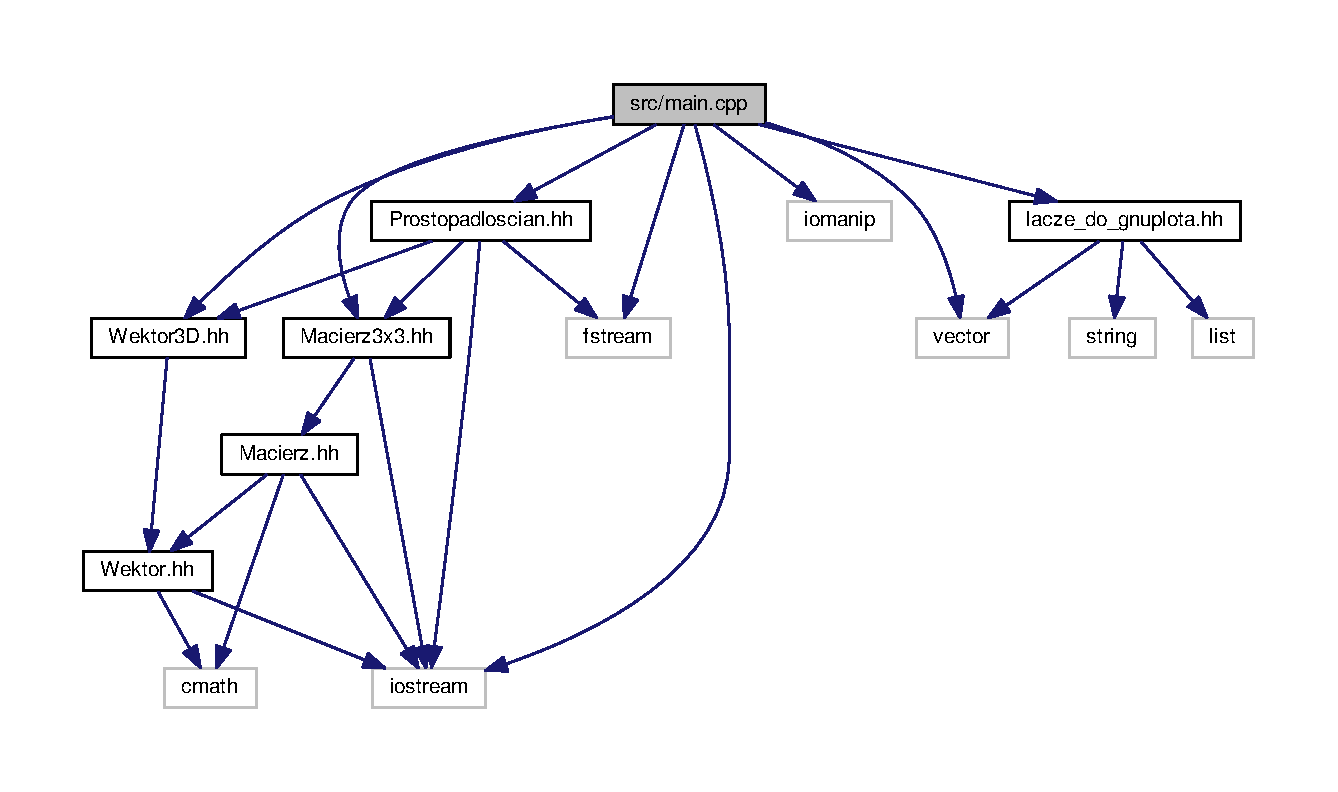
\includegraphics[width=350pt]{main_8cpp__incl}
\end{center}
\end{figure}
\subsection*{Classes}
\begin{DoxyCompactItemize}
\item 
struct \hyperlink{structelement__sekwencji}{element\+\_\+sekwencji}
\end{DoxyCompactItemize}
\subsection*{Macros}
\begin{DoxyCompactItemize}
\item 
\mbox{\Hypertarget{main_8cpp_a331949e395e085a8d60dfbf2239c87d7}\label{main_8cpp_a331949e395e085a8d60dfbf2239c87d7}} 
\#define {\bfseries D\+L\+U\+G\+O\+SC}~90
\end{DoxyCompactItemize}
\subsection*{Functions}
\begin{DoxyCompactItemize}
\item 
\mbox{\Hypertarget{main_8cpp_a2a0e843767aeea4f433a28b9c54f573a}\label{main_8cpp_a2a0e843767aeea4f433a28b9c54f573a}} 
void \hyperlink{main_8cpp_a2a0e843767aeea4f433a28b9c54f573a}{menu} ()
\begin{DoxyCompactList}\small\item\em Menu programu. \end{DoxyCompactList}\item 
\mbox{\Hypertarget{main_8cpp_ae66f6b31b5ad750f1fe042a706a4e3d4}\label{main_8cpp_ae66f6b31b5ad750f1fe042a706a4e3d4}} 
int \hyperlink{main_8cpp_ae66f6b31b5ad750f1fe042a706a4e3d4}{main} ()
\begin{DoxyCompactList}\small\item\em Czesc wykonywalna programu. \end{DoxyCompactList}\end{DoxyCompactItemize}


\subsection{Detailed Description}
Plik main 
\hypertarget{Prostopadloscian_8cpp}{}\section{src/\+Prostopadloscian.cpp File Reference}
\label{Prostopadloscian_8cpp}\index{src/\+Prostopadloscian.\+cpp@{src/\+Prostopadloscian.\+cpp}}


Plik zawiera dzialania na prostokacie.  


{\ttfamily \#include \char`\"{}Prostopadloscian.\+hh\char`\"{}}\newline
{\ttfamily \#include $<$iomanip$>$}\newline
Include dependency graph for Prostopadloscian.\+cpp\+:\nopagebreak
\begin{figure}[H]
\begin{center}
\leavevmode
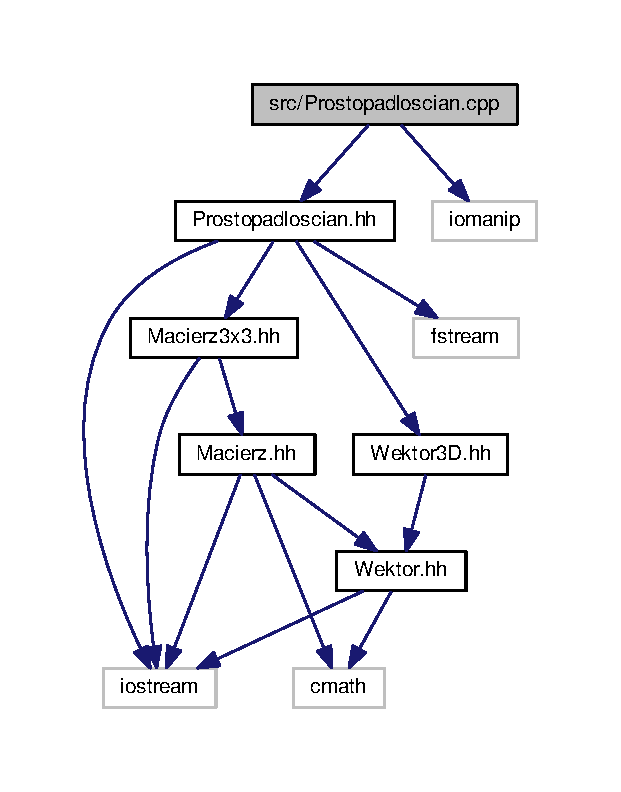
\includegraphics[width=298pt]{Prostopadloscian_8cpp__incl}
\end{center}
\end{figure}
\subsection*{Functions}
\begin{DoxyCompactItemize}
\item 
std\+::ostream \& \hyperlink{Prostopadloscian_8cpp_a0a77f9bb1cc3f07e11031b947e6e7322}{operator$<$$<$} (std\+::ostream \&Strm, const \hyperlink{classProstopadloscian}{Prostopadloscian} \&Pr)
\begin{DoxyCompactList}\small\item\em Przeciazenie operatora $<$$<$. \end{DoxyCompactList}\item 
void \hyperlink{Prostopadloscian_8cpp_a1fd5a38f6b20a1ea903c1ec882222dd6}{Zapis\+Do\+Strumienia} (ostream \&Strm\+Wy, \hyperlink{classWektor}{Wektor3D} Przesuniecie, \hyperlink{classProstopadloscian}{Prostopadloscian} \&Pr)
\begin{DoxyCompactList}\small\item\em Zapis danych do strumienia. \end{DoxyCompactList}\item 
void \hyperlink{Prostopadloscian_8cpp_a42155017ae1f49acb330164b11df2b97}{Zapis\+Do\+Strumienia} (ostream \&Strm\+Wy, \hyperlink{classMacierz}{Macierz3x3} Przesuniecie, \hyperlink{classProstopadloscian}{Prostopadloscian} \&Pr)
\begin{DoxyCompactList}\small\item\em Zapis danych do strumienia. \end{DoxyCompactList}\item 
bool \hyperlink{Prostopadloscian_8cpp_a140b1afdfa25067b9e9fcd7a738af090}{Zapis\+Wspolrzednych\+Do\+Pliku} (const char $\ast$s\+Nazwa\+Pliku, \hyperlink{classWektor}{Wektor3D} Przesuniecie, \hyperlink{classProstopadloscian}{Prostopadloscian} \&Pr)
\begin{DoxyCompactList}\small\item\em Zapis danych do pliku. \end{DoxyCompactList}\item 
bool \hyperlink{Prostopadloscian_8cpp_a7b6b375f9857993a4457fc37f47d585d}{Zapis\+Wspolrzednych\+Do\+Pliku} (const char $\ast$s\+Nazwa\+Pliku, \hyperlink{classMacierz}{Macierz3x3} Przesuniecie, \hyperlink{classProstopadloscian}{Prostopadloscian} \&Pr)
\begin{DoxyCompactList}\small\item\em Zapis danych do pliku. \end{DoxyCompactList}\end{DoxyCompactItemize}


\subsection{Detailed Description}
Plik zawiera dzialania na prostokacie. 



\subsection{Function Documentation}
\mbox{\Hypertarget{Prostopadloscian_8cpp_a0a77f9bb1cc3f07e11031b947e6e7322}\label{Prostopadloscian_8cpp_a0a77f9bb1cc3f07e11031b947e6e7322}} 
\index{Prostopadloscian.\+cpp@{Prostopadloscian.\+cpp}!operator$<$$<$@{operator$<$$<$}}
\index{operator$<$$<$@{operator$<$$<$}!Prostopadloscian.\+cpp@{Prostopadloscian.\+cpp}}
\subsubsection{\texorpdfstring{operator$<$$<$()}{operator<<()}}
{\footnotesize\ttfamily std\+::ostream\& operator$<$$<$ (\begin{DoxyParamCaption}\item[{std\+::ostream \&}]{Strm,  }\item[{const \hyperlink{classProstopadloscian}{Prostopadloscian} \&}]{Pr }\end{DoxyParamCaption})}



Przeciazenie operatora $<$$<$. 

Przeciążenie operatora przesuniecia bitowego w lewo sluzy do przekazania strumienia danych na podane wyjscie. \mbox{\Hypertarget{Prostopadloscian_8cpp_a1fd5a38f6b20a1ea903c1ec882222dd6}\label{Prostopadloscian_8cpp_a1fd5a38f6b20a1ea903c1ec882222dd6}} 
\index{Prostopadloscian.\+cpp@{Prostopadloscian.\+cpp}!Zapis\+Do\+Strumienia@{Zapis\+Do\+Strumienia}}
\index{Zapis\+Do\+Strumienia@{Zapis\+Do\+Strumienia}!Prostopadloscian.\+cpp@{Prostopadloscian.\+cpp}}
\subsubsection{\texorpdfstring{Zapis\+Do\+Strumienia()}{ZapisDoStrumienia()}\hspace{0.1cm}{\footnotesize\ttfamily [1/2]}}
{\footnotesize\ttfamily void Zapis\+Do\+Strumienia (\begin{DoxyParamCaption}\item[{ostream \&}]{Strm\+Wy,  }\item[{\hyperlink{classWektor}{Wektor3D}}]{Przesuniecie,  }\item[{\hyperlink{classProstopadloscian}{Prostopadloscian} \&}]{Pr }\end{DoxyParamCaption})}



Zapis danych do strumienia. 

Zapis wspolrzednych zbioru punktow do strumienia wyjściowego. Dane sa odpowiednio sformatowane, tzn. przyjęto notację stałoprzecinkową z dokładnością do 10 miejsca po przecinku. Szerokość wyświetlanego pola to 16 miejsc, sposób wyrównywania -\/ do prawej strony. 
\begin{DoxyParams}[1]{Parameters}
\mbox{\tt in}  & {\em Strm\+Wy} & -\/ strumien wyjsciowy, do ktorego maja zostac zapisane kolejne wspolrzedne. \\
\hline
\mbox{\tt in}  & {\em Przesuniecie} & -\/ ten parameter jest aby przekazac wektor przesuniecia \\
\hline
\mbox{\tt in}  & {\em \hyperlink{classProstopadloscian}{Prostopadloscian}} & -\/ ten parameter przekazuje oryginal obiektu bryly \\
\hline
\end{DoxyParams}
\mbox{\Hypertarget{Prostopadloscian_8cpp_a42155017ae1f49acb330164b11df2b97}\label{Prostopadloscian_8cpp_a42155017ae1f49acb330164b11df2b97}} 
\index{Prostopadloscian.\+cpp@{Prostopadloscian.\+cpp}!Zapis\+Do\+Strumienia@{Zapis\+Do\+Strumienia}}
\index{Zapis\+Do\+Strumienia@{Zapis\+Do\+Strumienia}!Prostopadloscian.\+cpp@{Prostopadloscian.\+cpp}}
\subsubsection{\texorpdfstring{Zapis\+Do\+Strumienia()}{ZapisDoStrumienia()}\hspace{0.1cm}{\footnotesize\ttfamily [2/2]}}
{\footnotesize\ttfamily void Zapis\+Do\+Strumienia (\begin{DoxyParamCaption}\item[{ostream \&}]{Strm\+Wy,  }\item[{\hyperlink{classMacierz}{Macierz3x3}}]{Przesuniecie,  }\item[{\hyperlink{classProstopadloscian}{Prostopadloscian} \&}]{Pr }\end{DoxyParamCaption})}



Zapis danych do strumienia. 

Zapis wspolrzednych zbioru punktow do strumienia wyjściowego. Dane sa odpowiednio sformatowane, tzn. przyjęto notację stałoprzecinkową z dokładnością do 10 miejsca po przecinku. Szerokość wyświetlanego pola to 16 miejsc, sposób wyrównywania -\/ do prawej strony. 
\begin{DoxyParams}[1]{Parameters}
\mbox{\tt in}  & {\em Strm\+Wy} & -\/ strumien wyjsciowy, do ktorego maja zostac zapisane kolejne wspolrzedne. \\
\hline
\mbox{\tt in}  & {\em Przesuniecie} & -\/ ten parameter jest aby przekazac macierz obrotu \\
\hline
\mbox{\tt in}  & {\em \hyperlink{classProstopadloscian}{Prostopadloscian}} & -\/ ten parameter przekazuje oryginal obiektu bryly \\
\hline
\end{DoxyParams}
\mbox{\Hypertarget{Prostopadloscian_8cpp_a140b1afdfa25067b9e9fcd7a738af090}\label{Prostopadloscian_8cpp_a140b1afdfa25067b9e9fcd7a738af090}} 
\index{Prostopadloscian.\+cpp@{Prostopadloscian.\+cpp}!Zapis\+Wspolrzednych\+Do\+Pliku@{Zapis\+Wspolrzednych\+Do\+Pliku}}
\index{Zapis\+Wspolrzednych\+Do\+Pliku@{Zapis\+Wspolrzednych\+Do\+Pliku}!Prostopadloscian.\+cpp@{Prostopadloscian.\+cpp}}
\subsubsection{\texorpdfstring{Zapis\+Wspolrzednych\+Do\+Pliku()}{ZapisWspolrzednychDoPliku()}\hspace{0.1cm}{\footnotesize\ttfamily [1/2]}}
{\footnotesize\ttfamily bool Zapis\+Wspolrzednych\+Do\+Pliku (\begin{DoxyParamCaption}\item[{const char $\ast$}]{s\+Nazwa\+Pliku,  }\item[{\hyperlink{classWektor}{Wektor3D}}]{Przesuniecie,  }\item[{\hyperlink{classProstopadloscian}{Prostopadloscian} \&}]{Pr }\end{DoxyParamCaption})}



Zapis danych do pliku. 

Zapis wspolrzednych zbioru punktow do pliku, z ktorego dane odczyta program gnuplot i narysuje je w swoim oknie graficznym. 
\begin{DoxyParams}[1]{Parameters}
\mbox{\tt in}  & {\em s\+Nazwa\+Pliku} & -\/ nazwa pliku, do którego zostana zapisane wspolrzędne punktów. \\
\hline
\mbox{\tt in}  & {\em Przesuniecie} & -\/ ten parameter jest aby przekazac wektor przesuniecia \\
\hline
\mbox{\tt in}  & {\em \hyperlink{classProstopadloscian}{Prostopadloscian}} & -\/ ten parameter przekazuje oryginal obiektu bryly \\
\hline
\end{DoxyParams}

\begin{DoxyRetVals}{Return values}
{\em true} & -\/ gdy operacja zapisu powiodła się, \\
\hline
{\em false} & -\/ w przypadku przeciwnym. \\
\hline
\end{DoxyRetVals}
\mbox{\Hypertarget{Prostopadloscian_8cpp_a7b6b375f9857993a4457fc37f47d585d}\label{Prostopadloscian_8cpp_a7b6b375f9857993a4457fc37f47d585d}} 
\index{Prostopadloscian.\+cpp@{Prostopadloscian.\+cpp}!Zapis\+Wspolrzednych\+Do\+Pliku@{Zapis\+Wspolrzednych\+Do\+Pliku}}
\index{Zapis\+Wspolrzednych\+Do\+Pliku@{Zapis\+Wspolrzednych\+Do\+Pliku}!Prostopadloscian.\+cpp@{Prostopadloscian.\+cpp}}
\subsubsection{\texorpdfstring{Zapis\+Wspolrzednych\+Do\+Pliku()}{ZapisWspolrzednychDoPliku()}\hspace{0.1cm}{\footnotesize\ttfamily [2/2]}}
{\footnotesize\ttfamily bool Zapis\+Wspolrzednych\+Do\+Pliku (\begin{DoxyParamCaption}\item[{const char $\ast$}]{s\+Nazwa\+Pliku,  }\item[{\hyperlink{classMacierz}{Macierz3x3}}]{Przesuniecie,  }\item[{\hyperlink{classProstopadloscian}{Prostopadloscian} \&}]{Pr }\end{DoxyParamCaption})}



Zapis danych do pliku. 

Zapis wspolrzednych zbioru punktow do pliku, z ktorego dane odczyta program gnuplot i narysuje je w swoim oknie graficznym. 
\begin{DoxyParams}[1]{Parameters}
\mbox{\tt in}  & {\em s\+Nazwa\+Pliku} & -\/ nazwa pliku, do którego zostana zapisane wspolrzędne punktów. \\
\hline
\mbox{\tt in}  & {\em Przesuniecie} & -\/ ten parameter jest aby przekazac macierz obrotu \\
\hline
\mbox{\tt in}  & {\em \hyperlink{classProstopadloscian}{Prostopadloscian}} & -\/ ten parameter przekazuje oryginal obiektu bryly \\
\hline
\end{DoxyParams}

\begin{DoxyRetVals}{Return values}
{\em true} & -\/ gdy operacja zapisu powiodła się, \\
\hline
{\em false} & -\/ w przypadku przeciwnym. \\
\hline
\end{DoxyRetVals}

%--- End generated contents ---

% Index
\backmatter
\newpage
\phantomsection
\clearemptydoublepage
\addcontentsline{toc}{chapter}{Index}
\printindex

\end{document}
